\documentclass{article}
\usepackage{graphicx} % Required for inserting images
\usepackage{James}
\usepackage{dynkin-diagrams}
\title{Lie Algebras and their Representations}
\author{James Hindmarch}
\usepackage{endnotes}
\setcounter{section}{0}
\date{October 2023}
\begin{document}

\begin{titlepage}
    \begin{center}
        \vspace*{1cm}
            
        \Huge
        Mathematical Tripos
            
        \vspace{0.5cm}
        \LARGE
        University of Cambridge
            
        \vspace{1.5cm}
        
        \Large
        Part III 
        \LARGE 

        \textbf{Lie Algebras and their representations}\\
        \vspace{1.5cm}
        Michaelmas, 2023
            
        \vspace{2cm}
        \Large \textit{Lectures by}\\
        \Large Prof. S. Martin\\

        \vspace{3cm}
        \large
        \textit{Notes by}\\
            James Hindmarch\\ \vspace{1.4cm}
        Email any corrections to: jah269@cam.ac.uk  
    \end{center}

\end{titlepage}
\tableofcontents
\section{Introduction}
A \underline{Lie group} is, fundamentally, a group that is also a smooth manifold, for example:
\[ GL_{n}, \hspace{0.1cm} SL_{n}, \hspace{0.1cm} SO_{n}, \hspace{0.1cm} Sp_{2n} \]
Over, for example, some infinite field, such as $\bbC$.
\ex $S^1 = \{ z \in \bbC \suchthat{|z| = 1} \}$ is the prototypical example of a Lie group. \gap 
Let $G$ be a Lie group. The \underline{Lie Algebra} of $G$ is the tangent space of $G$ at the identity, $e$, of $G$. That is to say: \[ \mathfrak{g} = T_{e} G. \] $\frakg$ is a vector space, but also has additional structure.\gap By taking a differential, we can turn the conjugation map:
\begin{align*}
    G &\to \Aut G\\
    g &\mapsto g (\widecdot) g^{-1}
\end{align*}
where $G$ is a Lie group, into a map $\ad$ (for adjoint):
\[ \ad : \frakg \to \End \frakg. \] This gives a bilinear map:
\begin{align*}
    [\widecdot, \widecdot] : \frakg \times \frakg &\to \frakg\\
    [x,y] &\mapsto \ad(x)(y)
\end{align*}
\ex If $G=GL_{n}(\bbR)$, then \[ \frakg = \frakgl_{n}(\bbR) = M_{n}(\bbR)\] \[ [x,y] = xy-yx \]
So far, so good, so what?
\begin{enumerate}
    \item[(a)] How do Lie algebras tell us about the structure of $G$?
    \begin{itemize}
        \item We'll define the \underline{root system} of $G$; this tells us about commutator relations in $G$ (See Carter's book for more)
        \item We'll define the \underline{Weyl group} of $\frakg$, e.g. the Weyl group of $GL_{n}(\bbC)$ is $\cong S_{n}$. This is basically to do with the fact that there is an embedding
        \[ S_{n} \hookrightarrow GL_{n}(\bbC)\] which is obtained via permutation matrices acting on a basis of $\bbC^{n}$.
    \end{itemize}
    Let $\mathcal{B} = \{ \text{upper triangular matrices in } GL_{n}(\bbC) \}$. Then $\exists$ Bruhat decomposition, which is: \[ GL_{n}(\bbC) = \disunion_{w \in S_{n}} \mathcal{B}w\mathcal{B}\]
    (i.e. the disjoint union of double cosets of $\mathcal{B}$.)
    \item[(b)] They tell us about the representation theory of $G$ and $\frakg$. For example, there is a bijection \[ \{\text{finite dim. } \bbC\text{-reps of } SL_{n}(\bbC)\} \longleftrightarrow \{\text{finite dim. } \bbC\text{-reps of the Lie algebra of } SL_{n}(\bbC)\}\] Where the Lie algebra of $SL_{n}(\bbC)$ is
    \[ \fraksl_{n}(\bbC) = \{A \in M_{n}(\bbC)| \, \tr(A)=0 \}. \]
    We will be able to describe the RHS completely (by listing all the representations).
    \item[(c)] They have applications in Algebraic Geometry. We can use Lie Algebras to build families of surfaces, or algebraic curves (See Slodowy's book for more).\gap
    We define the \underline{Dynkin diagram} of a semisimple Lie algebra, e.g.\[
    \dynkin E7 \]
    (This is the Dynkin diagram of "Type $E_{7}$"). This tells you about singularities on surfaces.
    \item[(d)] There are applications to Number theory: root systems and Weyl groups can help you to get the structure of groups over $\bbQ_{p}$ (the $p$-adics).\footnote{See the Iwahari-Matsumoto Paper} \gap
    There is the Local Langlands correspondence which predicts a relationship:
    \[ \text{Galois Theory of Local Fields} \longleftrightarrow \text{Complex Lie Theory} \]
    \item[(e)] There are also applications to applied maths, and that's all we'll say about that.
\end{enumerate}
\section{Basic Definitions and Examples}
Let $k$ be a field (most of the time this will be $\bbC$, but not always: we'll sometimes look at how things go wrong in fields with $\chr k > 0$.)
\begin{fancydefine}{Lie Algebra}
    A \textbf{Lie algebra} over $k$ is a vector space $\frakg$ over $k$ with a bilinear pairing
    \[
    [\widecdot, \widecdot]: \frakg \times \frakg \to \frakg \]
    which satisfies
    \begin{itemize}
        \item $[x,x]=0$
        \item $[x,[y,z]] + [y,[z,x]] + [z,[x,y]] = 0$ \hspace{1cm} (Jacobi Identity)
    \end{itemize}
\end{fancydefine}
    \textbf{\underline{Exercise:}} Check that these properties imply antisymmetry
    \[ [x,y] + [y,x] = 0 \]
\begin{fancydefine}{Lie subalgebra}
     A \textbf{Lie subalgebra} is a $k$-subspace $\frakh \subset \frakg$, such that $\frakh$ is closed under the Lie bracket of $\frakg$: \[
[x,y] \in \frakh \hspace{0.5cm} \forall x,y \in \frakh \]
\end{fancydefine}
\ex Let $V$ be finite-dimensional over $k$.
\begin{enumerate}
    \item[(a)] Let $\frakgl_{n}(V) = \End_{k}(V)$ with bracket \[
    [x,y]=xy-yx. \]
    Then it is clear that $[x,x]=0$, and you can check Jacobi yourself. \gap If we choose a basis for $V$, then we can identify $\frakgl_{n}$ with the space of $n\times n$ matrices over $k$, and then we can write $\frakgl(V)$ as $\frakgl_{n}$ (or $\frakgl_{n}(k)$ to emphasise the field, or just $M_{n}(k)$).
    \item[(b)] Let \[ \fraksl(V) = \{ x \in \frakgl(V) \, : \, \tr(x)=0 \}. \] This is clearly a subspace, since $\tr$ is linear. It is also closed under the Lie bracket, since $\tr$ is symmetric. That is to say:
    \[ \tr(xy-yx) = \tr(xy)-\tr(yx) = \tr(xy) - \tr(xy) = 0. \] Then $\dim(\fraksl(V)) = n^{2}-1$. And the standard basis for this is given by:
    \[ \{E_{ii} - E_{i+1,\, i+1} \,: 1 \leq i \leq n-1 \} \, \cup \, \{E_{ij} \, : \, i \neq j\}.  \]













    %LECTURE 2
    \newlec





    \item[(c)] Assume $\chr k \neq 2$. Suppose that $V$ is endowed with a symmetric bilinear form \[ [ \widecdot, \widecdot ] : V \times V \to k \]
    Let \[ \frakso(V) = \{ X \in \frakgl(V) \, : \, \langle Xv, w \rangle = - \langle v, Xw \rangle \, \forall v,w \in V \} \]
    If we use coordinates, then we have $\exists M \in GL(V)$ such that $\langle v,w \rangle = v^{\text{t}}Mw$, so then we have \[ \frakso(V) = \{ X \, : \, MX + X^{\text{T}}M =0 \}. \] Usually, we take \[ M = \begin{cases} 
    \begin{bmatrix}
        0 & I_{l} \\
        I_{l} & 0 \\
    \end{bmatrix}, & n=2l\\
    \\
    \begin{bmatrix}
        1 & 0 & 0\\
        0 & 0 & I_{l}\\
        0 & I_{l} & 0\\
    \end{bmatrix}, & n=2l+1
    \end{cases}
    \]
    These are the \textit{orthogonal Lie algebras}, denoted $\frakso_{n}$.\gap
    \textbf{Exercise:} What is their dimension? \gap
    (A note: $\mathfrak{o}_{n}$ and $\frakso_{n}$ are the same thing, since we "take tangent spaces at the identity," but the structure of $O(n)$ and $SO(n)$ do not differ at the identity, since the difference between them comes about because $O(n)$ has two connected components, so their Lie algebras are, in fact, identical).
    \remark If we let $n=2$, and take \[
    e=\begin{pmatrix} 0 & 1 \\ 0 & 0 \end{pmatrix}, \, f= \begin{pmatrix}
        0 & 0\\
        1 & 0
    \end{pmatrix}, \, h = \begin{pmatrix}
        1 & 0\\
        0 & -1
    \end{pmatrix},
    \] viewed as matrices (in $\fraksl_{2}(\bbC)$). This gives the standard basis from example (2). Then we have \[
    [e,f]=h, \, \, [h,e]=2e,\, \, [h,f]=-2f,\] and we will see that (in some sense) the structure of all \underline{semisimple} Lie algebras 'comes from' $\fraksl_{2}(\bbC)$.
\end{enumerate}
\begin{enumerate}
    \item[(d)] Assume $\chr k \neq 2$. Suppose $V$ has a skew-symmetric non-degenerate bilinear form: \[ \langle \widecdot, \widecdot \rangle: V \times V \to k\]
    i.e. such that
    \[ \langle v, w \rangle = - \langle w, v\rangle\]
    Then \[
    \fraksp = \{ x \in \frakgl(V) \, : \, \langle Xv,w \rangle = \langle v, Xw \rangle \} \]
    In coordinates, we take $\langle \widecdot, \widecdot \rangle$ to be the skew-symmetric form associated to: \[
    \begin{pmatrix}
        0 & I_{l}\\
        -I_{l} & 0\\
    \end{pmatrix}, \, \, \, \text{where $n=2l$}\]
    This is the \textit{symplectic Lie algebra}, denoted $\fraksp_{n}$ (where $n=2l$). \gap
    Note: $n$ \textit{must} be even, in order for $V$ to have a skew-symmetric bilinear form. \gap
    \textbf{Exercise:} Check (3) and (4) are indeed Lie subalgebras of $\frakgl(V)$. \\
    \item[(e)] Any space $V$ is a Lie algebra if we specify that \[ [v,w]=0, \, \, \forall v,w \in V \]
    These are called \textit{abelian} Lie algebras. Named for obvious reasons, (i.e. for linear Lie algebras, it means that matrices commute).
    \item[(f)]$\mathfrak{b}_{n}$: The set of upper triangular matrices (including the diagonal, i.e. non-strict upper triangular). This is the Borel subalgebra associated to the Borel subgroup of $GL_{n}$. \gap \textbf{Exercise}: What is the dimension of this Lie algebra, and why is it $\binom{n+1}{2}$?
    \item[(g)] $\mathfrak{n}_{n}$ The set of \textit{strictly} upper-triangular matrices. (The $\mathfrak{n}$ stands for nilpotent.)
\end{enumerate}
\section{Basic Representation Theory}
\begin{fancydefine}{Lie Algebra Homomorphism}
    A \underline{linear} transformation \[ \phi : \frakg \to \frakh \] between two Lie algebras is a \textbf{homomorphism} if: \[
    [\phi(x), \phi(y)] = \phi([x,y]) \, \, \forall x,y \in \frakg \]
    If $\phi$ is also bijective (i.e. is an isomorphism of vector spaces) then it is a Lie algebra \textbf{isomorphism}.
\end{fancydefine}
\begin{fancydefine}{Representation}
     Given a Lie algebra $\frakg$, we say that a \textbf{representation} of $\frakg$ is a Lie algebra homomorphism \[ \varphi : \frakg \to \frakgl(V) \] for some $V$. (We can write $\varphi = \varphi_{V}$ to emphasise the space).
\end{fancydefine}
\underline{Notation:}
\begin{itemize}
    \item We also call $V$ itself a 'representation,' or sometimes a $\frakg$-module.
    \item We write: $G \curvearrowright V$ and say $\frakg$ acts on $V$ (on the left).
    \item We usually write $x.v$ or $xv$ to mean $\varphi(x)(v)$
    \item The 'dimension' of the representation is $\dim V$.
\end{itemize}
\exs \hspace{0.1cm}
\begin{enumerate}
    \item The trivial representation: Let $\dim V = 1$, and let $\frakg \curvearrowright V$ via:\[
    x.v=0 \, \, \forall x \in \frakg, v \in V \]
    We call this representation the \textit{trivial representation}
    \item The defining representation: If $\frakg$ is a subalgebra of $\frakgl(V)$, then $\exists$ a natural inclusion: \[
    \iota: \frakg \to \frakgl(V).
    \] We call this inclusion the \textit{defining representation} of $\frakg$.
    \item The adjoint representation: Let $x \in \frakg$. Define \begin{align*}
        \ad(x) : \frakg &\to \frakg,\\
        y &\mapsto [x,y],
    \end{align*}
    then the map \begin{align*}
        \frakg &\to \frakgl(\frakg)\\
        x &\mapsto \ad x
    \end{align*}
    is the adjoint map. (Exercise: Show this is a Lie algebra homomorphism -- Use Jacobi, one line). \gap
    Note: Recall the earlier remark, the adjoint representation of $\fraksl_{2}(\bbC)$, with basis $\{e,h,f\}$ in that order, has:
    \begin{align*}
        \ad e &= \begin{bmatrix}
            0 & -2 & 0\\
            0 & 0 & 1\\
            0 & 0 & 0
        \end{bmatrix}\\
        \ad h &= \begin{bmatrix}
            2 & 0 & 0\\
            0 & 0 & 0\\
            0 & 0 & -2
        \end{bmatrix}\\
        \ad f &= \begin{bmatrix}
            0 & 0 & 0\\
            -1 & 0 & 0\\
            0 & 2 & 0 \\
        \end{bmatrix}
    \end{align*}
    \item If $V,W$ are representations, then so is $V \oplus W$ via: \[ x.(v,w) = (xv,xw). \]
    \item If $V$ is a representation of $\frakg$, then so is $V^{*}$ via: \[
    \forall x \in \frakg, \, v \in V, \, f \in V^{*}; \, (xf)(v) \to -f(x.v)\]
    Check this.
    \item If $V, W$ are representations of $\frakg$, then so is $\Hom(V,W)$ via:
    \[ \forall v \in V, \, x \in \frakg, \, f \in \Hom(V,W); \, (x.f)(v) = x.f(v) - f(x.v)\]
    Check this too.
\end{enumerate}
\begin{fancydefine}{$\frakg$-equivariance} 
    If $V,W$ are reps of $\frakg$, then a linear transformation \[ \varphi : V \to W \]
    is called $\frakg$\textbf{-equivariant} if \[ \forall x \in \frakg, \, v \in V, \, x.\varphi(v) = \varphi(x.v). \]
    We say $V,W$ are isomorphic as representations if there is a $\frakg$-equivariant isomorphism between them.
\end{fancydefine}
\begin{fancydefine}{Subrepresentation}
     A \textbf{subrepresentation} $V' \subseteq V$ is a subspace such that \[ \forall x \in \frakg, \, v \in V'; \, \,x.v \in V'.\]
\end{fancydefine}
\begin{fancydefine}{Irreducible} 
    We say that a representation is \textbf{irreducible} or \textbf{simple} if the only subrepresentations are $V$ \& $\mathbf{0}$ (but the $\mathbf{0}$ vector space is \textit{not} an irreducible representation).
\end{fancydefine}
\textbf{Exercise(s)} \begin{itemize}
    \item The trivial representation is irreducible.
    \item The defining and adjoint representations of $\fraksl_{2}(\bbC)$ are irreducible.
\end{itemize}







\newlec 
%LECTURE 3












\begin{fancydefine}{Completely reducible/Semisimple} 
    $V$ is a \textbf{completely irreducible} or \textbf{semisimple} representation if it decomposes as a sum of irreducible representations.
\end{fancydefine} 
\textbf{Exercise: }For V a representation, complete reducibility is equivalent to \[ \forall\, \text{subreps }W \subseteq  V, \, \, \exists W' \text{ such that } V' = W \oplus W'. \]
 If V is a representation, $W \leq V$ a subrepresentation, then \[ \frac{V}{W} \] is a representation of $\frakg$ via \[ x : (v + W) = xv + W \]
\section{Representation Theory of $\fraksl_{2}(\bbC)$}
Recall that \[ \fraksl_{2}(\bbC) = \{ X \, : \, \tr(X)=0 \}. \]
\textbf{Example: } Consider the Borel subalgebra of dimension 2, given by \[ \frakb_{2} = \{ \begin{pmatrix} a & b \\ 0 & c \end{pmatrix} \, : \, a,b,c \in \bbC \}.\] Then let $V = \spann\{\begin{pmatrix} 0 \\ 1 \end{pmatrix}, \, \begin{pmatrix}
    1 \\ 0
\end{pmatrix} \}$, the defining representation of $\frakb_{2}$. This is not completely irreducible (there is a similar example in II Representation theory). $\left< \begin{pmatrix}
    1 \\ 0
\end{pmatrix} \right>$ is a subrepresentation, but there is no complement subrepresentation by easy linear algebra.
\begin{fancydefine}{Faithful} A representation $V$ of a Lie algebra $\frakg$ is \textbf{faithful} if \[ \frakg \to \frakgl(V)\] is injective.
\end{fancydefine}
Henceforth, all Lie algebras and their representations are over $\bbC$ (unless stated otherwise). \gap Let $V$ be a representation of $\fraksl_{2}(\bbC)$, recall: \[e=\begin{pmatrix} 0 & 1 \\ 0 & 0 \end{pmatrix}, \, f= \begin{pmatrix}
    0 & 0\\
    1 & 0
\end{pmatrix}, \, h = \begin{pmatrix}
    1 & 0\\
    0 & -1
\end{pmatrix},\] 
We know three representations of $\fraksl_{2}(\bbC)$ already:\\
\begin{table}[h]
    \centering
    \begin{tabular}{c | c | c}
        Dim & Name & Action of $h$ \\ \hline
        $1$ & trivial & $0$\\ 
        $2$ & defining & $\begin{pmatrix}
            1 & 0 \\ 0 & -1 
        \end{pmatrix}$\\ \hspace{0.1cm} & \hspace{0.1cm} & \hspace{0.1cm} \\
        $3$ & adjoint & $\begin{pmatrix}
            2 & 0 & 0\\
            0 & 0 & 0\\
            0 & 0 & -2\\
        \end{pmatrix}$
    \end{tabular}
\end{table}
\begin{fancydefine}{$\lambda$-weight space} For $\lambda \in \bbC$ the $\mathbf{\lambda}$\textbf{-weight space} of $V$ is  \[ V_{\lambda} = \{ v \in V \, : \, hv=\lambda v\}.\]
\end{fancydefine}
The following are \textit{vector space sums} of \textit{weight-spaces}, \textbf{not} decompositions into irreducible representations.
\begin{itemize}
    \item The trivial is $V_{0}$
    \item The defining is $V_{1} \oplus V_{-1}$
    \item The adjoint is $V_{2} \oplus V_{0} \oplus V_{-2}$. Given by $\langle e \rangle \oplus \langle h \rangle \oplus \langle f \rangle$
\end{itemize}
\textbf{Actions:}\gap
Of $e$: for $v \in V_{\lambda}$, \begin{align*} h \cdot (ev) &= ([h,e] + eh)v\\
    &=(2ev) + \lambda e v
\end{align*}
So $h \cdot ev = (\lambda + 2)ev$. So $ev \in V_{\lambda + 2}$.
\gap
Of f: By a virtually identical argument, $fv \in V_{\lambda-2}$. So we have the following diagram: 
\begin{center}
\begin{tikzcd}
    \cdots &
    V_{\lambda-4} \arrow[r, bend left=50, "e"]
    & \arrow[l, bend left=50, "f"] V_{\lambda-2}
    \arrow[r, bend left=50, "e"]
    & \arrow[l, bend left=50, "f"] V_{\lambda}
    \arrow[r, bend left=50, "e"]
    & \arrow[l, bend left=50, "f"] V_{\lambda+2}
    \arrow[r, bend left=50, "e"]
    & \arrow[l, bend left=50, "f"] V_{\lambda+4} & \cdots
\end{tikzcd}
\end{center}
\begin{fancydefine}{Highest Weight Vector}
    If a non-zero $v \in V_{\lambda} \cap \ker(e)$ for some $\lambda$, then $v$ is called a \textbf{Highest Weight Vector} (or HWV) of weight $\lambda$. That is to say: \begin{align*}
    hv = \lambda v & & ev=0
\end{align*}
\end{fancydefine} 
\textbf{Example: } In the adjoint representation, $e$ is a highest weight vector of weight $2$.
\begin{fancylem}{} Suppose $v \in V_{\lambda}$ is a HWV, then $\forall n \geq 1$ \[ ef^{n}v = n(\lambda-n+1)f^{n-1}v\]
\end{fancylem}
\proof Easy induction on $n$ \gap Base Case: \[ (ef)v = ([e,f] +fe)v = (h + fe)v = hv = \lambda v. \] 
Inductive Step: Suppose this is true for $n=k-1$, then we have: \[ ef^{k-1}v = (k-1)(\lambda-(k-1)+1)f^{k-2}v. \]
Then: \begin{align*} ef^{k}v&=([e,f]f^{k-1} + fef^{k-1})v\\
    &=(h + fe). (f^{k-1}v)\\
    &=  (hf^{k-1}v) + (k-1)(\lambda - (k-1) + 1)f^{k-1}v\\
    &= (\lambda - 2(k-1))f^{k-1}v + (k-1)(\lambda - k + 2)f^{k-1}v\\
    &=k(\lambda - k + 1)f^{k-1}v
\end{align*}
\endproof
\begin{fancylem}{}
    Suppose $v \in V_{\lambda}$ is a HWV. Then $W=\spann\{v,fv,f^{2}v,\dots \}$ is a subrepresentation of $V$.
\end{fancylem}
\proof It suffices to show that if $w=f^{n}v$, then
    \begin{enumerate}
        \item[(i)] $ew \in W$
        \item[(ii)] $hw \in W$
        \item[(iii)] $fw \in W$  
    \end{enumerate}
(iii) Clearly true by definition of $W$. \gap (i) If $n>1$ this follows from Lemma 4.4 above, and if $n=0$ then $ew=0$ by definition of HWV. \gap (ii) $f^{n}w \in V_{\lambda -2n}$, so $hw = (\lambda-2n)w \in W$.
\endproof
\begin{fancyprop}{} If V is finite dimensional, it contains at least one highest weight vector (no claim about uniqueness).
\end{fancyprop}
\proof Choose any non-zero eigenvector $v$ of $h$. (This can always be done, since we're in $\bbC$ now). \gap Consider $v,ev,e^{2}v,\dots$. This set: \[ \{e^{n}v \, : \, ev \neq 0 \}\] is linearly independent, as the $e$ action changes the eigenvalue of $v$ when acted on by $h$. Therefore. as $V$ is finite dimensional, this set must be finite. So $\exists \, n$ such that $ e^{n}v \neq 0$, but $e^{n+1}v =0$. Therefore $e^{n}v$ is a highest weight vector, with weight $\lambda +2n$.
\begin{fancylem}{} Suppose $V$ is finite dimensional, and $v \in V_{\lambda}$ is a highest weight vector, then $\lambda \in \bbZ_{\geq0}$.
\end{fancylem}
\proof Any non-zero vectors of the form $f^{n}v$ must be linearly independent. So \[ \exists n\geq 0 \text{  s.t  } f^{n}v \neq 0 \text{  but  } f^{n+1}v=0\]
By ($4.4$) \[ 0 = (ef^{n+1})v = (n+1)(\lambda - n)f^{n}v \]
Therefore $f^{n}v \neq 0$, $n+1 \neq0$, so $\lambda=n$. \endproof Suppose that $V$ is irreducible, of dimension $n+1$. Then by (4.6), there is a HWV $v \in V_{\lambda}$, by (4.5), the span of $\{ v,fv,f^{2},\dots\}$ is a subrepresentation of $V$. So $\{v,fv,f^{2}v, \dots, f^{n}v\}$ is a basis, as the $f^{i}v$ are all linearly independent for $0 \leq i \leq n$. We know from (4.7) that $\lambda = n \in \bbZ_{\geq 0}$.
\begin{corr}{} If $V$ an irreducible representation of $\fraksl_{2}(\bbC)$ of dimension $n+1$, then there exists a basis $v_{0},v_{1},\dots v_{n}$ of $v$ such that
\begin{enumerate}
    \item[(i)] $hv_{i} = (n-2i)v_{i}$, that is: \[
        h =
        \begin{bmatrix}
          n & & & &\\
          & n-2 & & &\\
          & & \ddots & &\\
          & & & 2-n &\\
          & & & & n
        \end{bmatrix}
      \]
    \item[(ii)] $f_{v_{i}}=v_{i+1}$ for $0\leq i \leq n-1$, that is:\[
        f =
        \begin{bmatrix}
          0 & & & &\\
          1 & 0 & & &\\
          & 1 & 0 & &\\
          & & \ddots & \ddots  &\\
          & & & 1 & 0
        \end{bmatrix}
      \]
    \item[(iii)] $ev_{i} = \begin{cases}
        i(n-i+1)v_{i-1}, & i\geq 1\\
        0, & i=0 
    \end{cases}, \, \, \, \,$
    that is: \[
        e =
        \begin{bmatrix}
          0 & n & & &\\
            & 0 & 2(n-1) & &\\
            & & 0 & \ddots &\\
          & & & \ddots & n \\
          & & & & 0
        \end{bmatrix}.
      \]
\end{enumerate}
\end{corr}





















\newlec 
%LECTURE 4
\section{Irreducible modules for $\fraksl_{2}$}
\begin{remark}
    Let $V$ be an (n+1)-dimensional irreducible representation of $\fraksl_{2}$, $v \in V$ a highest weight vector. Then note: \[ (ef + fe + \frac{1}{2}h^{2})(v) = nv + \frac{n^{2}}{2}v = (\frac{n^{2}}{2}+n)v.\]
    This is a special operator, and we're going to see it three times very quickly.
\end{remark}
We write $V(n)$ for the unique irreducible representation of $\fraksl_{2}$ of dimension $n+1$.
\begin{fancydefine}{Weights}
    Given a representation $V$ of $\fraksl_{2}$, then \[ \{ \lambda \in \bbC \, : \, V_{\lambda} \neq 0 \}\] are called the \textbf{weights} of V.
\end{fancydefine}
Today, we will show \underline{Weyl's theorem} which states that the category of finite dimensional representations of $\fraksl_{2}(\bbC)$ is irreducible.
\begin{fancythm}{}
    Every finite dimensional representation of $\fraksl_{2}$ is completely reducible.
\end{fancythm}
This result, along with (4.8), says that to understand a representation of $\fraksl_{2}$, you essentially just need to understand the action of $h$. That is, the action of $h$ completely determines a finite dimensional representation of $\fraksl_{2}(\bbC)$.
\begin{ex}
    Suppose you have some $5$-dimensional representation of $\fraksl_{2}$, and that $\exists v \in V$ such that $hv = 3v$. This means that the weights will contain $3, 1, -1, -3$, so we must have \[ V = V(0) \oplus V(3), \] since $5=1+4$. (Dimension counting.) \endproof
\end{ex}
Before we prove (5.2), we need some facts. First of all, if $\frakg$ is an arbitrary Lie algebra, and \[ \varphi : \frakg \to \frakgl(V) \] is a representation of $\frakg$, and there is some $\sigma$ which commutes with $\varphi(x)$ $\forall x \in \frakg$. Then we have facts, which you should check:
\begin{enumerate}
    \item $\ker(\sigma - \lambda \id_{V})$ is a subrepresentation of $V$ for all $\lambda \in \bbC$.
    \item If $V$ is irreducible, then $\sigma$ is a scalar multiple of the identity. (Schur's Lemma).
\end{enumerate}
\begin{fancydefine}{Casimir element}
    Let $V$ be a finite dimensional representation of $\fraksl_{2}$. Then \[\Omega = (ef + fe + \frac{1}{2}h^{2}) \in \frakgl(V)\] is called the \textbf{Casimir element} (of $\fraksl_{2}$). In fact, $\Omega$ is central.
\end{fancydefine}
\begin{fancylem}{The Casimir element is central}
    If \[ \varphi : \fraksl_{2} \to \frakgl(V), \] then $\Omega$ commutes with $\varphi(x)$, $\forall x \in \fraksl_{2}$ (for $V$ finite dimensional).
\end{fancylem}
\proof
    To show $\Omega$ is central, show $e\Omega = \Omega e$, $f\Omega = \Omega f$, $h \Omega = \Omega h$. Just a mechanical check. 
\endproof
\begin{corr}{}
    If $V$ is an irreducible finite dimensional representation of $\fraksl_{2}$ then $\Omega$ acts on $V$ by a scalar.\\ \hspace{0.1cm}
\end{corr}
\proof Schur's Lemma. By the remark above, the scalar is $(\frac{n^2}{2} + n)$. \endproof

\textit{Proof of $\mathit{(5.2)}$}. The general case is done in Humphreys' book on page $63$. There's a different proof in Henderson's book: 5.2.1, 7.5.1. \gap
Let \[ \varphi : \fraksl_{2} \to \frakgl(V) \] be a finite dimensional representation of $\fraksl_{2}$. Let $W \leq V$ be a subrepresentation. Then we need to show $\exists U \leq V$ such that \[ V = W \oplus U. \]\gap 

\textit{Case 1.} $W$ has codimension $1$\footnote{$\frac{V}{W}$ has dimension $1$}. So we must have $\frac{V}{W} \cong V(0)$. \\

Subcases: \begin{enumerate}
    \item[(1)] W is trivial, so $\dim V = 2$, and there exists a basis of $V$ ($v_{1}, v_{2}$ such that $W=\bbC v_{1}$) with respect to which $\fraksl_{2}$ acts on $V$ by matrices which look like:
    \[ \begin{pmatrix}
        0 & * \\ 
        0 & 0
    \end{pmatrix}. \]
    We show $V \cong V(0) \oplus V(0)$ where the first $V(0)$ is $W$ and the second one is the $U$ that we are looking for.\\
    Note: \[ \left[ \begin{pmatrix}
        0 & x\\
        0 & 0
    \end{pmatrix},
    \begin{pmatrix}
        0 & y\\
        0 & 0
    \end{pmatrix} \right]=0 \, \, \forall x,y \in \bbC \] 
    Since $\varphi$ respects the bracket: \[ \varphi(h) = [\varphi(e),\varphi(f)]=0,\] \[ \varphi(e) = \frac{1}{2}[\varphi(h),\varphi(e)]=0, \] \[ \varphi(f) = \frac{1}{2}[\varphi(h), \varphi(f)]=0.\]
    So in other words, the action \textit{must} be trivial on the other factor, and that is the complement that we were after.\gap


    \item[(2)] $W \cong V(n)$ is irreducible, but nontrivial $(n > 0)$. Now we have: \[ \Omega \in \frakgl(V)\] We show $V=V(n) \oplus \ker(\Omega)$.\gap By Schur, and the fact that $W$ is irreducible, \textit{and} the fact that $\Omega$ acts on the quotient trivially (since codimension is $1$), there is a basis for $V$ such that $\Omega$ acts via: \[
    \begin{pmatrix}
        \lambda & & & & *\\
        & \lambda & & & *\\
        & & \ddots & & *\\
        & & & \lambda & *\\
        & & & & 0
    \end{pmatrix}\]
    $W$ is nontrivial, so $\ker \Omega \neq 0$, and it's now clear that \[ W \cap \ker \Omega = 0.\] So in other words, \[ V = W \oplus \ker \Omega.\]

    \item[(3)] Now let's take an arbitrary $W$. The idea now is to do induction on the $\dim V$. If $\dim V = 1$ then it is trivial, so that is already taken care of in subcase 1. So now assume $\dim V \geq 2$. \gap Take some subrepresentation $0 \neq W' \leq W$. As $\dim \left( \frac{W}{W'} \right) < \dim V$, and the codimension of $\frac{W}{W'}$ in $\frac{V}{W'}$ is $1$ (by, like, the third(?) isomorphism theorem, maybe it's the second), then by induction, we have: \[ \frac{V}{W'} = \frac{W}{W'} \oplus \frac{W''}{W'} \tag{1} \] for some subspace $W''$ of $V$ which contains $W'$, and is such that $\frac{W''}{W'}$ is a subrepresentation of $\frac{V}{W'}$.
    
    Then $W' \leq W''$ has codimension $1$ and morover $\dim W' < \dim V$. $W''$ is a subrepresentation of $V$, since $\frac{W''}{W'}$ being a subrepresentation implies that \[ xw \in W' \leq W'' \, \, \forall x \in \fraksl_{2}.\] Again by induction, $\exists U \leq W''$ such that \[ W'' = W' \oplus U. \tag{2} \] Then we claim that \[V = W \oplus U. \] We know already that $\dim U = 1$, and that $W \cap U \leq W \cap W'' = W'$, since we showed that (1) is a direct sum. But, by (2), as this sum is direct, $W \cap U \leq W' \cap U = 0$, and since $\dim U = 1$ and the codimension of $W$ in $V$ is $1$, we're done by counting dimensions (rank-nullity).
\end{enumerate}
\textit{Case 2.} Let $W$ be arbitrary. Recall from chapter $3$ the action on $\Hom(V,W)$: \[ (x \varphi)(v) = x(\varphi(v)) - \varphi(xv) \tag{3.3(6)}\]
Now we define \begin{align*}
    \mathbf{V} &= \{ \psi \in \Hom(V,W) \, : \, \psi |_{W} = \lambda \id_{W} \text{ for some } \lambda \in \bbC\},\\
    \mathbf{W} &= \{ \psi \in \mathbf{V} \, : \, \psi |_{W} = 0 \}.
\end{align*}
    Note that the codimension of $\mathbf{W}$ in $\mathbf{V}$ is $1$, and suppose \[\psi |_{W} = \lambda \id_{W}, \, x \in \fraksl_{2}, \, w \in W.\] Then \begin{align*} 
    (x\psi)(w) = x \psi(w) - \psi(xw) &= x(\lambda w) - \lambda (xw) \\
    &= 0.
\end{align*}
So $\mathbf{V}$ is a subrepresentation of $\Hom(V,W)$ threfore $\mathbf{W}$ is a subrepresentation. By case 1, $\exists 1-$dim subrepresentation $\mathbf{U}$ of $\mathbf{V}$ such that \[ \mathbf{V} = \mathbf{W} \oplus \mathbf{U}.\] Write $\mathbf{U} = \langle \gamma \rangle$ for some $\gamma \in \mathbf{V}$, so that $\gamma|_{W} = \lambda \id_{W}$, for some $0 \neq \lambda \in \bbC$. The claim is that (as vector spaces, and then as representations): \[ V = W \oplus \ker(\gamma).
\] where, we claim, that $U = \ker \gamma$.
\newlec
$W \cap \ker \gamma=0$, so by dimension counting, \[ \dim V = \dim W + \dim \ker \gamma.\] as $W= \im \gamma$. So we \textit{do} have a direct sum of vector spaces. Finally, we show that $\ker \gamma$ is a subrepresentation of $V$. Let $v \in \ker \gamma$ and take $x \in \fraksl_{2}$. $\mathbf{U}$ is a 1-dimensional representation of $\fraksl_{2}$, so it must be the trivial representation, since this is the only 1-dim representation of $\fraksl_{2}$.
Then we have 
\begin{align*}
    0 = (x \gamma)(v)&=x \gamma(v)-\gamma(xv)\\
    \Rightarrow x \gamma(v)&=\gamma(xv)\\
    \Rightarrow 0 &= \gamma(xv) \tag{$v \in \ker \gamma$}
\end{align*}
as required, since then $xv \in \ker \gamma$ for any $x \in \fraksl_{2}$, so it must be a subrepresentation. \endproof
\begin{remark}
    Proof only needed:
    \begin{itemize}
        \item The existence of $\Omega$, the Casimir element.
        \item Every 1-dimensional representation of $\fraksl_{2}$ is the trivial representation.
    \end{itemize}
\end{remark}
\begin{remark}
    Complete reducibility is \textit{rare}. It can fail for infinite dimensional Lie algebras, or \textit{simple Lie algebras} in positive characteristic fields.
\end{remark}
\textbf{Exercise: } Show that the adjoint representation of $\fraksl_{n}(\bbF_{p})$ on $gl_{n}(\bbF_{p})$ is not completely reducible, provided $p | n$. (Quite a hard exericse, apparently).
\section{Tensor products}
Given two finite dimensional vector spaces $V$, $W$; with bases $\{v_{1},\dots, v_{k}\}$, and $\{w_{1},\dots,w_{m}\}$ respectively. Recall that \[ V \otimes_{\bbC} W\] has basis \[ \{v_{i} \otimes w_{j} \, : \, 1\leq i \leq k, \, 1 \leq j \leq m\}.\]
\begin{fancydefine}{Tensor representation}
    If $V,W$ are representations of a Lie algebra $\frakg$, then so is $V \otimes W$ with \[ x\cdot(v \otimes w) = (x \cdot v) \otimes w + v \otimes (x \cdot w).\]
\end{fancydefine}
\begin{exs}\hspace{0.1cm}
    \begin{enumerate}
    \item[(1)] If $V,W$ representations of $\fraksl_{2}$, $v \in V_{\lambda}$, $w \in W_{\mu}$, then \[ h \cdot (v \otimes w) = (\lambda + \mu)(v \otimes w).\] In particular, the weights of $V \otimes W$ are: \[ \{ \lambda + \mu \, : \, \lambda \text{ a weight for } V, \mu \text{ a weight for } W\}.\]
    \item[(2)] Decomposition of $V(2) \otimes V(2) = V(2)^{\otimes 2}$:
    \begin{center}
        \begin{tabular}{c | c c c }
                & 2 & 0 & -2 \\ \hline
                2 & 4 & 2 & 0 \\ 
                0 & 2 & 0 & -2\\
                -2 & 0 & -2 & -4
        \end{tabular}
    \end{center}
    So $V(2)^{\otimes 2} = V(4) \oplus V(2) \oplus V(0)$.
    \item[(3)] If $v_{n}$ is a highest weight vector in $V(n)$, show that $v_{n} \otimes v_{m}$ is the highest weight vector in $V(n) \otimes V(m)$. \gap \textbf{Question: }Is there a general formula for decomposing $V(n) \otimes V(m)$?\gap
    \textbf{Answer: } Clebsch-Gordon formula \[V(n) \otimes V(m) = \bigoplus_{r=|n-m|}^{n+m} V(r),\] going up in $2$s\footnote{See Part II Representation Theory for more information}.
    \end{enumerate}



\end{exs}

\begin{fancydefine}{Symmetric power}
    The \textbf{nth Symmetric power is} \[ S^{n}(V) = \Sym^{n}(V)=SV= \frac{V \otimes V \otimes \dots \otimes V}{M_{n}}\] where $M_{n}=\langle u_{1} \otimes \dots \otimes u_{n} - u_{\sigma(1)} \otimes \dots \otimes u_{\sigma(n)} \, | \, \sigma \in S_{n}, u_{i} \in V \rangle$. \gap For example $n=2$, have $M_{2}=\{v\otimes u - u \otimes v\}$.
\end{fancydefine}
\textbf{Fact. } $M_{n}$ is a subrepresentation of $V \otimes \dots \otimes V$ whenever $V$ is a subrepresentation of $\frakg$, so $\Sym^{n}(V)$ is a subrepresentation. Prove this as an exercise.
\begin{ex}
    In $S^{2}V$, $v \otimes w = w \otimes v$. Therefore $S^{2}V$ has basis \[ \{v_{i} \otimes  v_{j} \, : \, i\leq j\}.\] Decomposing $S^{2}(V(2))$, we have $0 \neq e \otimes e \in S^{2}(V(2))$, so $V(4)$ is a subrepresentation, and in fact \[S^{2}(V(2)) = V(4) \oplus V(0)\]
\end{ex}
\begin{fancydefine}{Exterior/Alternating Power}
    The \textbf{nth exterior/alternating power} is \[\Lambda^{n} V = \frac{V^{\otimes n}}{N_{n}}\] where $N_{n} = \langle u_{1} \otimes \dots \otimes u_{n} \, : \, u_{i} \in V \, \forall i, \, u_{i}=u_{j} \text{ for some j} \rangle$.
\end{fancydefine}
\begin{ex} With $n=2$, we have $N_{2} = \langle v \otimes v \, : \, v \in V \rangle$. $N_{n}$ is a subrepresentation of $V^{\otimes n}$. Prove this. \gap \textbf{Notation. } Write (the coset of) $u_{1} \otimes \dots \otimes u_{n}$ as $u_{1} \wedge \dots \wedge u_{n}$.\gap Decompose \[ \Lambda^{2}(V(2)) \cong V(2). \] with basis \[ \{e \wedge f, e \wedge h, h \wedge f\}.\] 
\end{ex}
\textbf{Exercise. } Find the dimensions of symmetric/exterior powers.
\section{Results about semisimple Lie algebras}
First, let $\frakg$ be a semisimple Lie algebra over $\bbC$.
\begin{fancydefine}{Ideal}
    A subspace $I \subseteq \frakg$ is an \textbf{ideal} of $\frakg$ if \[ [x,y] \in I, \, \, \forall x \in \frakg,\, y\in I.\]
    \begin{itemize}
        \item Any ideal is a subalgebra
        \item If $I$ is an ideal, then $\frakg/I$ is a Lie algebra with bracket: \[ [x+I,y+I]=[x,y]+I.\] 
        \item $I$ is an ideal if and only if it is a subrepresentation of the adjoint representation of $\frakg$.
    \end{itemize}
\end{fancydefine}
\textbf{Examples. } \hspace{0.1cm}
    \begin{enumerate}
        \item[(1)] The \underline{centre} of $\frakg$ is \[ Z(\frakg) = Z = \{ x \in \frakg \, : \, [xy] = 0, \, \forall y \in \frakg \}.\] Check that this is an ideal (use Jacobi identity). Note $Z = \ker( \ad : \frakg \to \End \frakg)$.\gap
         \textbf{Remark. } If $Z(G)=0$, then the adjoint is faithful, and $\frakg$ can be embedded inside $\End \frakg$, so it can be regarded as a Lie subalgebra of $\frakgl_{n}$ for some $n$.
         \footnote{Therefore is a deep theorem of Ado (not proved here) that says that if $\charr k =0$ then any finite dimensional Lie algebra $\frakg$ embeds as a Lie subalgebra in $\frakgl_{n}$ for some $m$, but this embedding is necessarily from the adjoint. In fact, this is true in characteristic $p$ as well, due to Iwasawa.}
        \item[(2)] The derived subalgebra is \[ D(\frakg) =\langle [x,y] \, | \, x,y \in \frakg \rangle.\] This is an ideal. Recall that $\fraksl_{n}$ is a subalgebra of $\frakgl_{n}$. Show that, in fact, $\fraksl_{n}$ is the \textit{derived subalgebra} of $\frakgl_{n}$.
        \item[(3)] If \[ \phi : \frakg \to \frakh\] is a homomorphism. Then $\ker \phi$ is also an ideal (this shouldn't be too surprising).
    \end{enumerate}
\newlec
\begin{fancydefine}{Simple Lie algebra}
    The Lie algebra $\frakg$ is \textbf{simple} if \[ [\frakg, \frakg] \neq 0 \] and the only ideals of $\frakg$ are $0$ and $\frakg$.
\end{fancydefine}
\textbf{Examples. } \hspace{0.1cm}
    \begin{itemize}
    \item We can show $\fraksl_{n}$ is simple for $n \geq 2$.
    \item $\frakso_{n}$ is simple for $n \geq 5$.
    \item $\fraksp_{2l}$ for $l \geq 1$ is simple.
    \end{itemize}
    Try this now for $\fraksl_{2}(\bbC)$.\gap
\textbf{Note. } \begin{itemize}
    \item $\frakg$ simple $\Rightarrow$ $[\frakg,\frakg]=\frakg$.
    \item $\frakg$ simple $\Rightarrow$ every representation of $\frakg$ is either faithful or a direct sum of trivial representations.
\end{itemize}
So $\frakg$ simple $\Leftrightarrow$ the adjoint representation is irreducible.
\begin{fancydefine}{Semisimple Lie algebra}
    A Lie algebra $\frakg$ is \textbf{semisimple} if it is the direct sum of simple ideals. I.e. ideals which are themselves simple when viewed as Lie algebras.
\end{fancydefine}
For example $\frakso_{4} \cong \fraksl_{2} \oplus \fraksl_{2}$. We state a more "standard" definition of semisimple Lie algebras and then show it is equivalent to (7.3).
\begin{fancydefine}{Central series}
    The \textbf{Central series} (or lower central series) is the sequence of subalgebras \[ \frakg^{0} \supseteq \frakg^{1} \supseteq \frakg^{2} \supseteq \dots, \] where $\frakg^{0} = \frakg$ and $\frakg^{n} = [\frakg, \frakg^{n-1}]$. That is to say: \[ \frakg \supseteq [\frakg, \frakg] \supseteq [\frakg, [\frakg, \frakg]] \supseteq \dots. \]
\end{fancydefine}
\begin{fancydefine}{Derived series}
    The \textbf{Derived series} (or upper central series) for $\frakg$ is the sequence \[ \frakg^{(0)} \supseteq \frakg^{(1)} \supseteq \frakg^{(2)} \supseteq \dots, \] where $\frakg^{(0)} = \frakg$, $\frakg^{(n)} = \frakg^{(n-1)}, \frakg^{(n-1)}$. That is to say \[ \frakg \supseteq [\frakg, \frakg] \supseteq [[\frakg, \frakg], [\frakg, \frakg]] \supseteq \dots. \]
\end{fancydefine}
Note that: \begin{itemize}
    \item $\frakg^{(n)} \subseteq \frakg^{n}$
    \item $\forall n \, \, \frakg^{(n)}, \frakg^{n}$ are ideals, we will prove this:
\end{itemize}
\proof Induction on $n$, with $n=0$ clear. Let $x$,$y$ in $\frakg$, $\frakg^{n}$ respectively, then \[ [x,y] \in \frakg^{n-1}.\] Since $\frakg^{n-1}$ is an ideal, and $\frakg^{n} \subseteq \frakg^{n-1}$. But \begin{align*} \frakg^{n} &= \{ [x,y] \, : \, x \in \frakg, y \in \frakg^{n-1} \} \\
    &\supseteq \{ [x,y] \, : \, x \in \frakg, y \in \frakg^{n}
\end{align*}
Similarly, do $\frakg^{(n)}$. \gap \textbf{Examples. }
\begin{itemize}
    \item If $\frakg$ is simple, both series look like \[ \frakg \supseteq \frakg \supseteq \frakg \supseteq \dots.\]
    \item If $\frakg$ is abelian, both series look like \[\frakg \supseteq 0 \supseteq 0 \supseteq \dots.\] 
    \item Let \[ \frakn_{n} = \begin{pmatrix}
        0 & * & *\\
        0 & \ddots & *\\
        0 & 0 & 0
    \end{pmatrix} \subseteq \frakgl_{n}\]
    Central series for $\frakn_{n}$: \[ \left\{ \begin{pmatrix}
        0 & * & * & *\\
        0 & \ddots & * & *\\
        0 & 0 & \ddots & *\\
        0 & 0 & 0 & 0
    \end{pmatrix} \right\} \supseteq \left\{ \begin{pmatrix}
        0 & 0 & * & *\\
        0 & \ddots & \ddots & *\\
        0 & 0 & \ddots & 0\\
        0 & 0 & 0 & 0
    \end{pmatrix} \right\} \supseteq \left\{ \begin{pmatrix}
        0 & 0 & 0 & *\\
        0 & \ddots & \ddots & 0\\
        0 & 0 & \ddots & 0\\
        0 & 0 & 0 & 0
    \end{pmatrix} \right\} \supseteq \dots \] If $n=3$ this is the Heisenberg Lie algebra. Moreover, this central series eventually becomes $0$, so we call it nilpotent, as a result of the following definition.
\end{itemize}
\begin{fancydefine}{Nilpotent/Solvable}
    If $\frakg^{n}=0$ for some $n$, then $\frakg$ is called \textbf{nilpotent}. If $\frakg^{(n)}=0$ for some $n$, then $\frakg$ is called \textbf{solvable}.
\end{fancydefine}
\textbf{Exercise. } Show $\frakb_{n}$ is solvable but not nilpotent $(n \geq 2)$. By the note to (7.5), we have that nilpotent $\Rightarrow$ solvable.\gap Next result allows the theory of compex semisimple Lie algebras to go very far with minimal work.
\begin{fancythm}{Lie's theorem}
    Let $k=\bbC$. Let $\frakg \leq \frakgl(V)$ be a Lie subalgebra. Suppose that $\frakg$ is solvable. Then there exists a common eigenvector for all the elements of $\frakg$: \[ \exists 0 \neq v \in V \, \text{ s.t. } \, \forall x \in \frakg, \, \, \exists \lambda_{n} \in \bbC \, \text{ s.t. } \, xv = \lambda_{n}v\]
\end{fancythm}
\proof See Humphrey, Theorem 4.1. Just a two page linear algebra hack.
\begin{corr}{}
    There exists a basis for $V$ such that every element is upper triangular. In fact, using Lie's theorem and an inductive argument, we can show that there is a chain of subspaces of $V$ such that \[ 0 = V_{0} \leq V_{1} \leq V_{2} \leq \dots \leq V_{n} =V, \] with $\dim V_{i}=i$ and $\frakg(V_{i}) \subseteq V_{i}$ for each $i$ (this is called a maximal flag). Taking basis of $V$ such that $V_{i} = \spann (e_{1}, \dots, e_{i})$, we have that $\frakg$ can be represented by upper triangular matrices, and so using such a basis \[ \frakg \leq \frakb_{n}.\]
\end{corr}
\proof Non-examinable. Probably also in Humphreys' book somewhere. 
\begin{fancyprop}{}
    Suppose $I$, $J$ ideals of $\frakg$, then \begin{enumerate}
        \item If $\frakg$  solvable, then any subalgebra, or quotient of $\frakg$ is solvable.
        \item If $I$ is solvable, and $\frac{\frakg}{I}$ is solvable, then so is $\frakg$.
        \item If $I$ is solvable and $J$ is solvable, then $I+J$ is solvable too.
    \end{enumerate}
\end{fancyprop}
\proof \hspace{0.1cm}
\begin{enumerate}
    \item Obvious from the definition of solvability.
    \item Choose $n$ such that \[\left(\frac{\frakg}{I}\right)^{(n)}=0\] So $\frakg^{(n)} \subseteq I$. Now we have \[\frakg^{(n+m)} \subseteq I^{(m)}\] for each $m \geq 0$, and since $I$ is solvable, we're done.
    \item Note that \[ \frac{(I+J)}{J} \cong \frac{I}{I \cap J}.\] The RHS is solvable by 1, and $J$ is solvable by assumption, and $\frac{(I+J)}{J}$ is therefore solvable. By 2, $I+J$ also solvable
\end{enumerate}
\endproof
\begin{fancydefine}{Radical}
    The \textbf{Radical} of $\frakg$, $\rad (\frakg)$ is the maximal solvable ideal of $\frakg$. It is the sum of all the solvable ideals of $\frakg$.
\end{fancydefine}
\begin{fancydefine}{Trace form}
    If $\phi : \frakg \to \frakgl(V)$ is a finite dimensional representation of $\frakg$, then the \textbf{Trace form} of $V$: \begin{align*} 
        (\widecdot, \widecdot) : \frakg \times \frakg &\to \bbC\\
        (x,y) &\mapsto \tr(\phi(x)\phi(y))
    \end{align*}
\end{fancydefine}
\textbf{Exercise. } \begin{enumerate}
    \item $\phi$ a representation of $\frakg$ $\Rightarrow$ $(\widecdot, \widecdot)_{V}$ is symmetric and bilinear.
    \item $([x,y],z)_{V} = (x,[y,z])_{V}$, called "Invariance."
\end{enumerate}
\begin{fancydefine}{Killing form}
    The \textbf{Killing form} $K(\widecdot, \widecdot)$ is the trace form attached to the adjoint representation, \[ K(x,y) = \tr( \ad(x), \ad(y)) = (x,y)_{\ad}.\]
    Also, we have that \[ K([x,y],z) = K(x,[y,z]),\] and we will use this a lot. (Easy to prove using linearity and cycle-invariance of trace).
\end{fancydefine}
\newlec \begin{fancythm}{}
    The following are equivalent for a finite dimensional Lie algebra $\frakg$ \begin{enumerate}
        \item $\frakg$ is semisimple (as defined in 7.3)
        \item $\rad (\frakg) = 0$
        \item The Killing form on $\frakg$ is non-degenerate. (Cartan-Killing criterion).
    \end{enumerate}
\end{fancythm}
\begin{remark*}
    $\rad(\frac{\frakg}{\rad(\frakg)})=0$ (A solvable ideal of $\frac{\frakg}{\rad(\frakg)})$) would lift to give an ideal $J$ of $\frakg$ containing $\rad(\frakg)$ with $\frac{J}{\rad(\frakg)}$ solvable
    \begin{align*}
        &\Rightarrow J \text{ solvable} \therefore J \subseteq \rad(\frakg)\\
        &\Rightarrow \frac{\frakg}{\rad(\frakg)} \text{  semisimple}
    \end{align*}\hspace{0.1cm}\\
    \textbf{Levi's Theorem. }(not proved here) Says that if $\chr k = 0$ and $\frakg$ is finite dimensional, then there is a Lie subalgebra $\frakg'$ such that \[ \frakg' \cap \rad(\frakg)=0\] and also \[\frakg = \frakg' \oplus \rad(\frakg).\] Thus \[ \frakg \cong \frac{\frakg}{\rad{\frakg}} \] is a semisimple Lie algebra. What this is saying is that, considering the following short exact sequence. \[ 0 \rightarrow \rad(\frakg) \rightarrow \frakg \rightarrow \frac{\frakg}{\rad(\frakg)} \rightarrow 0 \] splits, i.e. there exists $\frakg' \subseteq \frakg$ which maps into $\frac{\frakg}{\rad(\frakg)}$. This is called the Levi decomposition and $\frakg'$ is the Levi subalgebra of $\frakg$.\gap This result fails in $\chr k = p$ and for $\dim \frakg = \infty$.
\end{remark*}
\begin{fancylem}{}
    Let $\frakg$ be a Lie algebra, then \begin{enumerate}
        \item If $I$ is an ideal of $\frakg$, then so is the derived algebra $[I,I]$
        \item $\rad(\frakg)=0 \Leftrightarrow \frakg$ has no non-trivial abelian ideals.
    \end{enumerate}
\end{fancylem}
\proof \hspace{0.1cm} \begin{enumerate}
    \item If $x, y \in I$, $z \in \frakg$, we need to show \[ [z,[x,y]] \in [I,I]. \] The obvious thing to try is Jacobi, which gets us \[ [z,[x,y]] = -[x,[y,z]] - [y,[z,x]] \] then both summands on the right hand side have the inner bracket containing something in $I$, so the overall inner bracket is in $I$, and since these are bracketed with something which is also contained in $I$. Therefore, each overall expression is in $[I,I]$ Therefore the left hand side must also be in $[I,I]$.
    \item It's clear that any abelian ideal must be solvable. For the other direction, we have that if $I$ is solvable then the last non-zero term in the derived series for $I$ will be abelian. (Done by contrapositive both ways).
\end{enumerate}
\endproof
Let \[ \frakg^{\perp} = \{ x \in \frakg : K(x,y)=0, \, \, \forall y \in \frakg \}. \] This is an ideal, to show why: take $x \in \frakg^{\perp}$ and $y,z \in \frakg$. Then we need to show that \[ K([x,y],z])=0.\] But \[K([x,y],z) = K(x,[y,z]) = 0\] since $x \in \frakg^{\perp}$.
\begin{fancylem}{}
    Let $I$ be an ideal of $\frakg$ and let $K_{I}$ be the killing form of $I$. Then \[ K_{I}(x,y)=K(x,y), \, \, \forall x,y \in I. \]
\end{fancylem}
\proof Choose a basis of $I$ and extend to a basis for $\frakg$. Let $x,y \in I$, then with respect to this basis: \[ \ad(x) = \begin{pmatrix}
    A & * \\
    0 & 0
\end{pmatrix} \] where $A= \ad(x)|_{I}$. And similarly for $\ad(y)$. Then we have \[ K_{I}(x,y) = \tr(AB) = \tr(\ad(x),\ad(y))=K(x,y).\]
\begin{fancythm}{Cartan's criterion (for solvability)}
Suppose $\frakg$ is a subalgebra of $\frakgl(V)$, for $V$ a finite dimensional $\bbC$-space. If $K(x,y)$ is identically zero on $\frakg \times [\frakg,\frakg]$ then $\frakg$ is solvable. (This is saying that $\frakg^{(1)}\leq \frakg^{\perp})$.
\end{fancythm}
\proof A big linear algebra hack, in Humphreys 4.3, uses Lie's theorem and Jordan decomposition (which we will cover next chapter). Not a very hard proof\footnote{apparently}, just very long. This fails in $\chr k = p$ as well. \endproof
\begin{corr}{}
    \hspace{0.1cm} \begin{enumerate}
        \item If $\frakg = \frakg^{\perp}$ then $\frakg$ is solvable.
        \item If $\frakg$ is simple, then $\frakg^{\perp}=0$
        \item $\frakg^{\perp}$ is solvable for any finite dimensional $\frakg$.
    \end{enumerate}
\end{corr}
\proof \hspace{0.1cm}
\begin{enumerate}
    \item Consider the adjoint \[ \ad : \frakg \to \frakgl(V) \] The image $\ad (\frakg)$ is $\frakg$ modulo the kernel, so \[ \ad(\frakg) = \frac{\frakg}{Z(\frakg)}.\] $Z(\frakg)$ is solvable since it's abelian. Since $\frakg = \frakg^{\perp}$, Cartan's criterion (7.16) implies $\ad(\frakg)$ is solvable. So by (7.9), $\frakg$ must be solvable.
    \item $\frakg^{\perp}$ is an ideal, so either $\frakg^{\perp}=0$ (in which case we're done) or $\frakg^{\perp}=\frakg$, but then $\frakg$ is solvable by what we've just proved, which contradicts the fact that $\frakg$ is simple.
    \item $(\frakg^{\perp})^{\perp} = \frakg^{\perp}$ by (7.15) and basic properties of this ideal, so by 1. which we just proved, $\frakg^{\perp}$ is solvable. 
\end{enumerate}
\endproof
\textit{Proof of (7.13). }\begin{enumerate}
    \item[$(2) \Rightarrow (3)$:] $\frakg$ is a solvable ideal in its own right, so $\frakg^{\perp} \subseteq \rad(\frakg)$ which is assumed to be $0$, so $\frakg^{\perp}=0$
    \item[$(3) \Rightarrow (2)$:] Let $A$ be an abelian ideal of $\frakg$. We claim $A \subseteq \frakg^{\perp}$. Let $x \in A, y \in \frakg$. Choose a basis for $A$ and extend to $\frakg$. Then \[ \ad(x)= \begin{pmatrix}
        0 & *\\
        0& 0
    \end{pmatrix}\] 
    \[ \ad(y) = \begin{pmatrix}
        * & *\\
        0 & *
    \end{pmatrix}\] So $\tr(\ad(x)\ad(y))=0$, therefore $A=0$. And if $\rad(\frakg) \neq 0$ then $\frakg^{\perp}\neq 0$.
    \item[(2)\, \& (3) $\Rightarrow $(1):] If $\frakg$ is simple, then we're done. If not, then choose some minimal non-trivial ideal $I$. Let \[ \frakg_{I} = \{ x \in \frakg \, : \, K(x,y)=0 \, \forall y \in I \}\] This is an ideal of $\frakg$ (prove this). \gap \textbf{Claim 1: } $\frakg = I \oplus \frakg_{I}.$ \gap Since $I$ is simple (by minimality) and being non-abelian by (2), we know that \[ I \cap \frakg_{I} \subseteq I^{\perp} = 0.\] Consider the map \[ \frakg \xrightarrow{\simeq} \frakg^{*} \xrightarrow{\text{restrict}} I^{*}\] \[ x \to K(x, \widecdot) \to K|_{I^{*}}(x, \widecdot).\] The kernel of this map is $\frakg_{I}$, which prove the claim. We then repeat this argument with $g_{I}$ (choosing some minimal ideal of $g_{I}$). We can do this because (Exercise:) any ideal of $\frakg_{I}$ must be an ideal of $\frakg$ and so $\rad(\frakg_{I})=0$. \gap \textbf{Claim 2:} $(g_{I})^{\perp}=0$. Since if $\alpha \in (g_{I})^{\perp}$ then $x \in \frakg^{\perp}$
    
    \item[(1) $\Rightarrow$ (2)] Write $\frakg = \oplus I_{j}$, $I_{j}$ simple ideals. Let $\pi_{j}$ be projection onto $I_{j}$. 
\end{enumerate}
\endproof
\newlec \textbf{Exercise: } If $J$ is an ideal of $\frakg$, then $\pi_{j}(J)$ is an ideal of $I_{j}$\gap 
Now if $A \subseteq \frakg$ is an abelian ideal of $\frakg$, then $\pi_{j}(A)$ is an abelian ideal of $I_{j}$, so $\pi_{j}(A)=0 \, \forall j$ so $A=0$.
\begin{fancythm}{Weyl}
    Any finite dimensional representation of a semisimple Lie algebra is completely reducible.
\end{fancythm}
\idea Remember in the $\fraksl_{2}$ case, where we used the Casimir element, there is a general idea of a Casimir element for a general semisimple Lie algebra. This is how we prove this claim.
\proof The main ingredient is this new generalised Casimir element. \gap \textbf{Exercise: } Any ideal or quotient of a semisimple Lie algebra is also semisimple.
\begin{fancydefine}{General Casimir element}
    Take any representation \[ \phi : \frakg \to \frakgl(V)\] a finite dimensional irreducible representation of a semisimple Lie algebra $\frakg$. Then without loss of generality, assume that $\phi$ is faithful, otherwise just work with $\frac{\frakg}{\ker \phi}$. By Cartan-Killing criterion, $(-,-)$ the trace form, is non degenerate. Pick basis $x_{1}, \dots , x_{n}$ of $\frakg$. Since the trace form is non-degenerate, we can also pick a dual basis $y_{1}, \dots, y_{n}$. Then let \[ \Omega_{\phi} = \sum \phi(x_{i})\phi(y_{i}).\]
    In Humphreys' book, this is called \textit{the} \textbf{Casimir element} of $\phi$. Note \begin{itemize}
        \item $\Omega_{\phi}$ is an endomorphism of $V$
        \item $\Omega_{\phi}$ commutes with $\phi(x)$, $\forall x \in \frakg$.
    \end{itemize}
\end{fancydefine}
By Schur's Lemma, $\Omega_{\phi}$ is a scalar multiple of the identity on $V$, and $\tr(\Omega_{\phi)}) = \sum_{i} \tr(\phi(x_{i})\phi(y_{i})) = \dim \frakg$ and it's also clear that $\Omega_{\phi}$ is independent of the basis of $\frakg$ which we chose. \gap
\textbf{Example. } Let $\frakg = \fraksl_{2} \leq \frakgl_{2}$, with $V= \bbC^{2}$, and $\phi : \frakg \to \frakgl(V)$ is the defining representation of $\fraksl_{2}$, then take $\{e, f, h\}$, the standard basis of $\fraksl_{2}$. The dual basis relative to the trace form is $\{f, \frac{1}{2}h, e \}$. Then \[ \Omega_{\phi} = ef + \frac{1}{2}h^{2} +fe = \begin{pmatrix}
    \frac{3}{2} & 0 \\ 
    0 & \frac{3}{2}
\end{pmatrix}. \] The $\frac{3}{2}$ comes from $3$ being the dimension of the algebra, and $2$ being the dimension of the representation. 
The proof of Weyl's theorem follows the same as for $\fraksl_{2}$, but with this general casimir element.
\section{Jordan decomposition}
First, two observations: \begin{itemize}
    \item If $\frakg$ is a simple Lie algebra, and $\phi : \frakg \to \frakgl(V)$ is a finite dimensional representation, then $\phi(\frakg) \subseteq \fraksl(V)$. This is because $[\frakg, \frakg] = \frakg$, so \[\phi(g) = \phi([\frakg, \frakg]) = [\phi(\frakg),\phi(\frakg)] \subseteq [\frakgl(V), \frakgl(V)] = \fraksl(V).\]
    \item Recall that if $x \in \frakgl(V)$, then there is a basis of $V$ such that $x$ is a block diagonal, with Jordan blocks of form:\[
    \begin{pmatrix}
        \lambda & 1 & 0 & \dots &  0\\
        0 & \lambda & 1 & \dots & 0\\
        0 & 0 & \ddots & \ddots & 0\\
        0 & 0 & 0 & \ddots &  1\\
        0 & 0 & 0 & 0 & \lambda
    \end{pmatrix}\]
\end{itemize}
\begin{fancydefine}{Nilpotent/Semisimple elements}
    We say a element $x$ is \textbf{nilpotent} if $x^{n}=0$ for some $n$ and we say an element is \textbf{semisimple} if the roots of its minimal polynomial are distinct (i.e. it is diagonalisable).
\end{fancydefine}
\begin{fancyprop}{Jordan Decomposition}
    If $x \in \frakgl(V)$, and $V$ finite dimensional, then
    \begin{enumerate}
        \item There are unique $x_{s}, x_{n} \in \frakgl(V)$ with $x_{s}$ semisimple, $x_{n}$ nilpotent, and $x= x_{n} + x_{s}$ and $[x_{n},x_{s}]=0$.
        \item There exist polynomials $p_{s},p_{n} \in \bbC[T]$ without constant terms such that $x_{s} = p_{s}(x)$, $x_{n} = p_{n}(x)$ and $x_{s}$, $x_{n}$ commute with anything which commutes with $x$.
        \item If $A \leq B \leq V$ are subspaces, and $x: B \to A$, then $x_{s}$ and $x_{n}$ also map $B \to A$.
    \end{enumerate}
    The decomposition $x=x_{n}+x_{s}$ is called the (additive) Jordan(-Chevalley) decomposition of $x$. $x_{n}$ and $x_{s}$ are called the nilpotent part/semisimple part of $x$ respectively.
\end{fancyprop}
\proof Routine Linear Algebra (Done in Humphreys). \endproof
\textbf{Example. } If $x$ is represented by a single Jordan block, then \[ x_{s} = \begin{pmatrix}
    \lambda & 0 & 0 & 0\\
    0 & \lambda & 0 & 0\\
    0 & 0 & \ddots & 0\\
    0 & 0 & 0 & \lambda
\end{pmatrix} 
\] and \[ x_{n} = \begin{pmatrix}
    0 & 1 & 0 & 0 &\\
    0 & 0 & \ddots & 0\\
    0 & 0 & 0 & 1 &\\
    0 & 0 & 0 & 0
\end{pmatrix}.\]
Why is this a valuable thing to know? \gap Suppose $\frakg$ is a finite dimensional Lie algebra. Then we have an adjoint representation \[ \ad : \frakg \to \frakgl(V)\] for $V$ finite dimensional. Then if $x \in \frakgl(V)$ is nilpotent, so is $\ad(x)$ (prove this). Similarly, if $x$ is semisimple, then so is $\ad(x)$ (prove this too).
\begin{fancylem}{}
    Let $x \in \frakg \leq \frakgl(V)$ with $\dim V <\infty$. Then $x= x_{s} + x_{n}$ is its Jordan decomposition. Then \[\ad(x) = \ad(x_{s}) + \ad(x_{n})\] is the Jordan decomposition of $\ad(x)$ in $\frakgl(V)$.
\end{fancylem}
\proof $\ad(x_{s})$ and $\ad(x_{n})$ are respectively semisimple and nilpotent. They commute since \[ [\ad x_{s}, \ad x_{n}] = \ad([x_{s},x_{n}]) = 0\] By uniqueness in (8.2) the Jordan decomposition must be $\ad x = \ad x_{s} + \ad x_{n}$. \endproof
\begin{fancythm}{}
    Suppose $\frakg$ is semisimple and a subalgebra of $\frakgl(V)$ and $x \in \frakg$. Then $x_{s}, x_{n} \in \frakg$.\\ \hspace{0.1cm}
\end{fancythm}
\proof Let \[N(\frakg) = \{ y \in \frakgl(V) \, : \, [y,z] \in \frakg \, \, \forall z \in \frakg \},\]
be called the \textbf{normalizer} of $\frakg$ in $\frakgl(V)$. We claim that \begin{enumerate}
    \item $N(\frakg)$ is a subalgebra of $\frakgl(V)$ which contains $\frakg$ as an ideal.
    \item $x_{s}$ and $x_{n}$ are in $N(\frakg)$
\end{enumerate}
Claim 1 is clear by the definition of $N(\frakg)$. \gap
 For 2, we have that for $z \in \frakg$ we have $[x_{s},z] = \ad(x_{s})(z) = \ad(x)_{s}(z)$ and (by 8.2 part 2), this is in $\frakg$, since it is a polynomial in $\ad(x)$ with no constant term. 
 \gap Let $W$ be an irreducible subrepresentation of $V$, and define \[ \frakg_{W}=\{y \in \frakgl(V) \, : \, yw \in W \, \, \forall w \in W, \, \text{and} \, \tr(y)_{W}=0 \}. \]
Where $\tr(y)_{W}$ is the trace of the restriction of $y$ to $W$. Then we claim that \[ \frakg \leq \frakg_{W}.\]
$W$ is a subrepresentation, therefore $W$ must be stabilised by $\frakg$. The image of $\frakg$ in $\frakgl(W)$, call this $\bar \frakg$, must also be stabilised, then this is also semisimple.\gap
Therefore \[ [\bar \frakg, \bar \frakg] = \bar \frakg, \] therefore every element of $\bar \frakg$ is a sum of commutators (where the trace of every commutator must be $0$ by the definition of $\frakg_{W}$). Therefore $\frakg \leq \frakg_{W}$. 
Thus $\tr(y|_{W})=0$. Note $x_{s},x_{n}$ are polynomials in $x$, therefore, if $x$ stabilises something then $x_{s}$ and $x_{n}$ must stabilise it as well. Also $\tr(x_{n}|_{W}) = 0$, since $x_{n}|_{W}$ is nilpotent. Then \[ \tr(x_{s}|_{W}) = \tr(x|_{W}- x_{n}|_{W}) = \tr(x|_{W}) - \tr(x_{n}|_{W}) = 0. \] Therefore $x_{s},x_{n} \in \frakg_{W}$.
\gap Then to finish, we need to show that $x_{s}$ and $x_{n}$ are in $\frakg$. Define \[ \frakg' = N(\frakg) \cap \left( \bigcap_{W\leq V,\,\, W \,\text{irred}} \frakg_{W} \right). \]
And we claim $\frakg = \frakg'$, so that since $x_{s}$ and $x_{n}$ are in all of the $\frakg_{W}$ in the intersection, they must also lie in $\frakg'$ and thus in $\frakg$. \gap
Since $\frakg' \leq N(\frakg)$, $\frakg$ is an ideal of $\frakg'$. Then $\frakg$ is a subrepresentation of $\frakg'$ under the adjoint representation of $\frakg$. By Weyl's theorem (7.18) applied to $\frakg'$ \footnote{We know it is semisimple since we have a homomorphism to it from a semisimple Lie algebra, thus we can apply Weyl's theorem.}, $\frakg' = \frakg \oplus U$ as representations of $\frakg$ for some subrepresentation $U$. \gap
\textbf{Claim:} $U=0$. Take $u \in U$. We have $[u,\frakg] \subseteq \frakg$ as $\frakg$ is an ideal of $\frakg'$. But $\ad \frakg U \leq U$\footnote{since the adjoint acts faithfully.}, so $[u,\frakg] \subseteq U \cap \frakg = 0$. \gap Therefore $u$ commutes with every element of $\frakg$. Hence $u$ is a $\frakg$-homomorphism $V \to V$. So $u$ stabilises every irreducible subrepresentation $W$, so by Schur's lemma, we have \[ u|_{W} = \lambda \id_{W} \] for some scalar $\lambda$. Now $\tr(u|_{W})=0$ for all irreducible $W \leq V$ because $u \in \frakg_{W}$ for each $W$. Therefore \[ \tr(\lambda \id_{W}) = 0 \Rightarrow \lambda = 0 \Rightarrow u|_{W}=0.\] Finally, \[V \cong \bigoplus_{i} W_{i} \, \, \, \, \, \, \text{   some irreducibles $W_{i}$.}\] Therefore $u=0$.
\endproof
For $\frakg$ as in statement, we can define an \say{abstract} Jordan decomposition by \[ \ad(x) = \ad(x)_{s} + \ad(x)_{n}.\]
As $\ad$ is faithul, for $\frakg$ semisimple, we have \[ \frakg \cong \ad \frakg \leq \frakgl(\frakg).\] By (8.4) $\ad(x)_{s}, \ad(x)_{n} \in \ad(\frakg)$, hence are of the form $\ad(x_{s}), \ad(x_{n})$ for some elements $x_{s}, x_{n} \in \frakg$. \[ \ad x = \ad (x_{s} + x_{n}) \Rightarrow x = x_{s}+x_{n}\] by faithfulness.\gap 
Suppose $\frakg \leq \frakgl(V)$, for some $V$. Write $x=x_{s}+x_{n}$. By (8.3), $\ad(x_{s})=\ad(x)_{s}$, $\ad(x_{n}) = \ad(x)_{n}$. 
So the \say{abstract} decomposition we just gave agrees with the original definition.
\begin{corr}{}
    Let a representation \[ \varphi : \frakg \to \frakgl(V) \] be any representation of a semisimple Lie algebra $\frakg$. Let $x \in \frakg$ have Jordan decomposition $x=x_{s}+x_{n}$. Then \[ \varphi(x)_{s}=\varphi(x_{s})\] and \[ \varphi(x)_{n} = \varphi(x_{n})\] defines a Jordan decomposition of $\varphi(x)$.
\end{corr}
\proof Omitted. \footnote{In the 2015 notes by Stewart. It is his \say{Corollary 5.11}. \textit{Needs} semisimplicity, \textit{definitely needs} to be over $\bbC$.}
\begin{center} \large \textbf{End of Introduction} \normalsize \end{center}
There is a section $9$, but it rears its head later. On to section $10$.
\setcounter{section}{9}
\section{Cartan subalgebras and root space decompositions}
Here, as usual, $\frakg$ is some finite dimensional, semisimple Lie algebra over $\bbC$.
\begin{fancydefine}{Toral/Cartan subalgebra}
    A subalgebra $\frakt \subseteq \frakg$ is \textbf{toral} if \begin{enumerate}
        \item $\frakt$ is abelian.
        \item $\ad x$ is semisimple for all $x \in \frakt$.
    \end{enumerate}
    A maximal toral subalgebra is called a maximal torus or a \textbf{Cartan subalgebra} (CSA).
\end{fancydefine}
\begin{remark*}
    Many authors, including Humphreys, define Cartan subalgebras as nilpotent subalgebras which are equal to their normalizers in $\frakg$. This is equivalent to the definition above.
\end{remark*}
\begin{exs*}\hspace{0.1cm}
    \begin{enumerate}
        \item $\frakg \leq \fraksl_{n}, \frakgl_{n}$, then $\frakt = \{$diagonal matrices in $\frakg\}$ is a maximal torus.
        \item Similarly for $\frakso_{n}, \fraksp_{2n}$.
    \end{enumerate}
\end{exs*}
\begin{fancylem}{}
    Let $t_{1}, \dots, t_{n} : V \to V$ be pairwise commuting $(t_{i}t_{j} = t_{j}t_{i})$ semisimple endomorphisms of $V$ (f.d. over $\bbC$). Let \[ \lambda = (\lambda_{1}, \dots, \lambda_{n}) \in \bbC^{n}.\]
    Then set \[V_{\lambda}=\{ v \in V \, : \, t_{i}(v) = \lambda_{i}v, \, \, \forall 1 \leq i \leq n \} \]
    (the simultaneous eigenspaces for all $t_{i}$). Then \[ V = \bigoplus_{\lambda \in \bbC^{n}} V_{\lambda}.\] 
\end{fancylem}
\proof Induction on $n$. 
\gap \underline{$n=1$}: \gap This follows since $t_{1}$ is semisimple, so the diagonalisability means that $V$ has a basis of $t_{1}$-eigenvectors, so decomposes as $t_{1}$-eigenspaces. 
\gap \underline{$n>1$}: \gap We know by induction \[ V = \bigoplus_{\lambda' \in \bbC^{n-1}} V_{\lambda'}\] for the action of $t_{1}, \dots, t_{n-1}$. Then since $t_{i}$ commute, \[t_{n}(V_{\lambda'}) = V_{\lambda'} \, \, \forall \lambda'.\] So decomposing each $V_{\lambda'}$ for $t_{n}$ (exactly as in the $n=1$ case), we're done. 
\endproof
\begin{fancylem}{}
    Any $\frakg$ contains a Cartan subalgebra.\\ \hspace{0.1cm}
\end{fancylem}
\proof We need something called Engel's\footnote{Not that one, also he's called Engel, not Engels. However, they do both have first name Friedrich.} theorem, which is on sheet 2 as a further problem. We also need Zorn's lemma.
 \gap Recasting (10.2), suppose $\frakh \leq \frakgl(V)$ with a basis of commuting semisimple elements $t_{1}, \dots, t_{n}$. Then when we write $\lambda \in \bbC^{n}$, we mean it to correspond to the element of $\frakh^{*}$ (the dual) given by \[ t_{i} \mapsto \lambda_{i}.\] Then \[V_{\lambda} = \{ v \in V \, : \, hv = \lambda(h)v \, \, \forall h \in \frakh \}. \] 
In our situation, fix $\frakt \leq \frakg$ a Cartan subalgebra, then \[ \frakg = \bigoplus_{\lambda \in \frakt^{*}} \frakg_{\lambda},\] where \[ \frakg_{\lambda} = \{ x \in \frakg \, : \, [t,x] = \lambda(t)x, \, \, \forall t \in \frakt \}. \]
\endproof
\begin{fancydefine}{Roots/Root Space}
    Let \[ \Phi = \{ \alpha \in \frakt^{*} \setminus \{0 \} \, : \, \frakg_{\alpha} \neq 0 \}. \] The elements of $\Phi$ are the \textbf{roots} of $\frakg$ with respect to $\frakt$. If $\alpha \in \Phi$, $\frakg_{\alpha}$ is called a \textbf{root space} and \[ \frakg = \frakg_{0} \oplus \sum_{\alpha \in \Phi} \frakg_{\alpha}. \] is the \textbf{root space decomposition} or \textbf{Cartan decomposition} of $\frakg$.
\end{fancydefine}
\begin{fancyprop}{}\hspace{0.1cm}
    \begin{enumerate}
        \item For all $\alpha, \beta \in\ \frakt^{*}$, $[\frakg_{\alpha}, \frakg_{\beta}] \subseteq \frakg_{\alpha + \beta}$.
        \item If $\alpha \in \Phi$, then if $x \in \frakg_{\alpha}$, $\ad(x)$ is nilpotent.
        \item If $\alpha + \beta \neq 0$, $K(\frakg_{\alpha},\frakg_{\beta}) = 0$ for all $\alpha, \beta \in \frakt^{*}$
    \end{enumerate}
\end{fancyprop}
\proof \hspace{0.1cm} \begin{enumerate}
    \item Take $x \in \frakg_{\alpha}$, $y \in \frakg_{\beta}$, $t \in \frakt$. We have from the Jacobi identity that 
    \begin{align*} 
        [t,[x,y]] &= -[x,[y,t]] - [y,[t,x]]\\
        &= [x,[t,y]] - \alpha(t)[y,x]\\
        &= \beta(t)[x,y] + \alpha(t)[x,y]\\
        &= (\alpha + \beta))(t)[x,y]
    \end{align*}
    \item Use 1, and the finite dimensionality of $\frakg$.
    \item If $\alpha + \beta \neq 0$, then have that \[ \exists t \in \frakt \text{ such that } (\alpha + \beta)(t) \neq 0.\] So then fix such a $t$ and fix $x \in \frakg_{\alpha}$, $y \in \frakg_{\beta}$. Then 
    \begin{align*}
        \alpha(t)K(x,y) &= K([t,x],y)\\
        &= -K([x,t],y)\\
        &= -K(x,[t,y])\\
        &= -\beta(t)K(x,y)
    \end{align*}
    Which implies $(\alpha + \beta)(t)K(x,y)=0$. Therefore $K(x,y)=0$.
\end{enumerate}
\endproof
\begin{corr}{}\hspace{0.1cm}
    \begin{enumerate}
        \item $K|_{\frakg_{0} \times \frakg_{0}}$ is non-degenerate.
        \item If $\alpha \in \Phi$, then $-\alpha \in \Phi$.
    \end{enumerate}
\end{corr}
\proof \hspace{0.1cm} \begin{enumerate} \item If $z \in \frakg_{0}$ and $K(z,y)=0$ for all $y \in \frakg_{0}$, then by (10.5(3)) $\frakg_{0}$ is orthogonal to $\frakg_{\alpha}$ for $\alpha \neq 0$. If $x \in \frakg$ then we can write $x=x_{0} + \sum_{\alpha \in \Phi}x_{\alpha}$ with $x_{\alpha} \in \frakg_{\alpha}$. By linearity $K(z,x)=0$ for all $x \in \frakg$. Since $K$ is non-degenerate on $\frakg$, we must have $z=0$.
    \item Similar to above.
\end{enumerate}
\endproof
\begin{fancyprop}{}
    \[\frakg_{0}= \frakt \]
\end{fancyprop}
\proof Humphreys (8.2) \endproof
\begin{corr}{}
    $K|_{\frakt \times \frakt}$ is non-degenerate. In particular \begin{align*}
        \frakt &\to \frakt^{*}\\
        x &\mapsto K(x, \widecdot)
    \end{align*}
    is an isomorphism.
\end{corr}
\proof Let inverse be $\lambda \mapsto t_{\lambda}$, then $t_{\lambda} \in \frakt$ (called the coroot associated to $\lambda$ is defined by \[ K(t_{\lambda},x) = \lambda(x)\] for all $x \in \frakt$.
\endproof
\begin{exs*} \hspace{0.1cm}
    \begin{enumerate}
        \item $\frakg = \fraksl_{2}$, \[ \frakt = \left\langle \begin{pmatrix}
            1 & 0\\ 
            0 & -1
        \end{pmatrix}=h
        \right\rangle \] Define $\alpha \in \frakt^{*}$ by $\alpha(h)=2$. Then $\frakg_{\alpha} = \langle e \rangle$, $\frakg_{-\alpha}=\langle f \rangle$ and $\fraksl_{2} = \frakt \oplus \frakg_{\alpha} \oplus \frakg_{-\alpha}$.
        \item Let $\frakg = \fraksl_{3}$. Take \[ h_{1} = \begin{pmatrix}
            1 & &\\
            & -1 &\\
            & & 0
        \end{pmatrix}\] and \[ h_{2} = \begin{pmatrix}
            0 & &\\
            & 1 &\\
            & & -1\\
        \end{pmatrix}\] and let $\frakt = \langle h_{1}, h_{2} \rangle$. Let $\alpha_{i} \in \frakt^{*}$ be such that $\alpha_{i}(\diag(a_{1},a_{2},a_{3}))=a_{i}$ Then \[ \fraksl_{3} = \frakt \oplus \frakg_{\alpha_{1}-\alpha_{2}} \oplus \frakg_{\alpha_{1}-\alpha_{3}} \oplus \frakg_{\alpha_{2}-\alpha_{1}} \oplus \frakg_{\alpha_{2}-\alpha_{3}} \oplus \frakg_{\alpha_{3}-\alpha_{1}} \oplus \frakg_{\alpha_{3}-\alpha_{2}}\] where $\frakg_{\alpha_{i}-\alpha_{j}} = \langle e_{ij} \rangle.$ Try decomposing the adjoint this way.
        \item Try $\frakg = \fraksl_{n}$, $\frakt = $ diagonals in $\frakg$, then try $\frakg = \frakso_{2n}, \frakso_{2n+1},\fraksp_{2n}$.
    \end{enumerate}
\end{exs*}
\begin{fancyprop}{}
    If $\alpha \in \Phi$ is a root, $e_{\alpha} \in \frakg_{\alpha}$, then $\exists f_{\alpha} \in \frakg_{-\alpha}$ such that \[ \frakm_{\alpha} = \langle e_{\alpha}, f_{\alpha}, h_{\alpha} \rangle=[e_{\alpha},f_{\alpha}] \cong \fraksl_{2}.\] We're saying that every semisimple Lie algebra is \say{made out of} $\fraksl_{2}$'s.
\end{fancyprop}
First, note that if $t \in \frakt$ satsifies $\alpha(t)=0$ for all $\alpha \in \Phi$, then $t=0$. Since, if $\alpha \in \Phi$ and $x \in \frakg_{\alpha}$ then \[ 0 = \alpha(t)(x) = [t,x].\] Since a toral subalgebra is abelian, this holds in all of $\frakg$. $t \in Z(\frakg) = \{ 0 \}$. This gives us the following lemma.
\begin{fancylem}{}
    $\Phi$ spans $\frakt^{*}$
\end{fancylem}
\proof If not $\exists t \neq 0$ such that $\alpha(t)=0$ for all $\alpha \in \Phi$ which is false. \endproof
\textit{Proof of 10.9.}\hspace{0.1cm}\gap
\textbf{Claim 1:} $[\frakg_{\alpha},\frakg_{-\alpha}]$ is $1$-dimensional. \gap
Take $x \in \frakg_{\alpha}$, $y \in \frakg_{-\alpha}$, so $[x,y] \in \frakt$. Let $t \in \frakt$. So \[ K([x,y],t) = K(x,[y,t]) = -K(x,[t,y]) = \alpha(t)K(x,y)\]
Therefore $[x,y]=K(x,y)t_{\alpha} \in \langle t_{\alpha} \rangle.$ Therefore we know that $\dim [\frakg_{\alpha, \frakg_{-\alpha}}] \leq 1,$ but then \[ \exists x,y \text{ such that } K(x,y) \neq 0\] since $K$ is non-degenerate. Therefore the dimension must be $1$. \gap 
\textbf{Claim 2:} $\alpha(t_{\alpha}) \neq 0$. \gap 
Since the Killing form is non-degenerate, and rescaling is possible, we may choose $x \in \frakg_{\alpha}$ and $y \in \frakg_{-\alpha}$ such that $K(x,y)=1$. Then \[ [x,y] = K(x,y) t_{\alpha} = t_{\alpha}\] and we have \[ [t_{\alpha}, x] = \alpha(t_{\alpha})x, \, \, [t_{\alpha},y]= -\alpha(t_{\alpha})y.\] Therefore $\langle \{x,y,t_{\alpha} \} \rangle$ is a subalgebra, say $\frakh$, of $\frakg$. Assume that $\alpha(t_{\alpha})=0$. Since \[ [\frakh, \frakh] = \langle t_{\alpha} \rangle, \] this means that $\frakh$ is a solvable algebra.
Now \[ \ad : \frakg \to \frakgl_{\frakg},\] and we know $\frakh$ embeds into a solvable subalgebra of $\frakgl(\frakg)$, with respect to which \[ \ad(\frakh) \subseteq \{ \text{Upper triangular matrices} \}, \] and $\ad(t_{\alpha}) = [ \ad x, \ad y]$ is a stricly upper triangular matrix. Consider $\ad(t_{\alpha})$ is nilpotent, but then by semisimplicity (of the algebra), $\ad(t_{\alpha})$ is semisimple. Therefore \[\ad(t_{\alpha} = 0.\] Therefore $t_{\alpha} \in Z(\frakg) = \{0 \}$. \gap
\textbf{Claim 3:} $[[\frakg_{\alpha},\frakg_{-\alpha}],\frakg_{\alpha}] \neq 0.$ \gap 
If $x \in \frakg_{\alpha}, y \in \frakg_{-\alpha}$ with $K(x,y) \neq 0$, then for all $z \in \frakg_{\alpha}$: \[ [[x,y],z] = [K(x,y)t_{\alpha},z] = K(x,y)\alpha_{t_{\alpha}}z, \] which is non-zero if $z \neq 0$.\gap
\textbf{Claim 4: } \newlec If $\alpha \in \Phi$, $e_{\alpha} \in \frakg_{\alpha}$, then $\exists f_{\alpha} \in \frakg_{-\alpha}$ such that \[ \frakm_{\alpha} = \langle e_{\alpha}, f_{\alpha},h_{\alpha} = [e_{\alpha}, f_{\alpha}] \rangle \cong \fraksl_{2}.\] Take an element $e_{\alpha} \in \frakg_{\alpha}$ in the root space, and find $f_{\alpha} \in \frakg_{-\alpha}$ such that \[ K(e_{\alpha},f_{\alpha}) = \frac{2}{\alpha(t_{\alpha})}.\] Then define \[ h_{\alpha} = \frac{2}{K(t_{\alpha},t_{\alpha})}.\] Check that the $\fraksl_{2}$ relations hold: \begin{align*}
    [e_{\alpha},f_{\alpha}] &= K(e_\alpha , f_\alpha )t_\alpha = h_\alpha\\
    [h_{\alpha},e_{\alpha}] &= \frac{2}{\alpha(t_{\alpha})}[t_{\alpha},e_{\alpha}] = 2e_{\alpha}.\\
\end{align*}
and similarly \[ [h_{\alpha},f_{\alpha}] = -2f_{\alpha}. \] So this is indeed isomorphic to $\fraksl_{2}$. The set $\{e_{\alpha},f_{\alpha},h_{\alpha}\}$ is called a $\fraksl_{2}$-triple. \gap 
\textbf{Exercise: } Show that \say{weights add}: if $\frakg$ is semisimple with root space decomposition \[ \frakg = \frakt \oplus \bigoplus_{\alpha} \frakg_{\alpha}, \] and $V,W$ are representations of $\frakg$, which therefore have corresponding weight spaces $V_{\alpha}$ and $W_{\alpha}$. Then \begin{enumerate}
    \item $\frakg_{\alpha} V_{\beta} \subseteq V_{\alpha +\beta}.$
    \item  $V_{\alpha} \otimes W_{\beta} \subseteq (V \otimes W)_{\alpha + \beta}.$
\end{enumerate}
\begin{fancylem}{}\hspace{0.1cm}
    \begin{enumerate}
        \item If $V$ is a finite dimensional representation for $\frakg$, then $V|_{\frakm_{\alpha}}$ is a finite dimensional representation.
        \item If $\beta \in \Phi$ or $\beta = 0$, then let \[ V = \oplus \frakg_{\beta + c \alpha},\] where the direct sum is taken over all $c \in \bbC$ such that $\beta + c \alpha \in \Phi$. This is a representation of $\frakm_{\alpha}$ via restriction of the adjoint.
    \end{enumerate}
\end{fancylem}
\proof \hspace{0.1cm}
\begin{enumerate}
    \item Clear by generic facts about representations and restrictions.
    \item Clear from (10.5)
\end{enumerate}
\endproof
\begin{fancydefine*}{Root string}
     We call $V$ as obtained in Lemma 10.11 the $\mathbf{\alpha}$\textbf{-root string through }$\beta$.
\end{fancydefine*}
\begin{fancyprop}{}
    Let $\alpha \in \Phi$. The root spaces $\frakg_{\pm \alpha}$ are 1-dimensional. Moreover the multiples of $\alpha$ which lie in $\Phi$ are $\pm \alpha$.
\end{fancyprop}
\proof If $c \alpha \in \Phi$, then $h_{\alpha}$ takes $c \alpha(h_{\alpha})=2c$ as an eigenvalue. The eigenvalues of $h_{\alpha}$ are integral. Either $c \in \bbZ$ or $c \in \bbZ + \frac{1}{2}$. \gap 
Let \[ V = \frakt \oplus \bigoplus_{c \alpha \in \Phi} \frakg_{c \alpha}.\] Let $K = \ker \alpha \leq \frakt^{*} $. It is easy to check that $K \oplus \frakm_{\alpha}$ is a $\frakm_{\alpha}$ subrepresentation of $V$\footnote{Since $\frakm_{\alpha}$ acts trivially on $K$, so when we take the direct sum we still get a representation.}. 
By Weyl's theorem, as a representation of $\frakm_{\alpha}$, $V$ must split as \[ V = K \oplus \frakm_{\alpha} \oplus W,\] where $W$ is a complementary subrepresentation of $V$. Assume either of the conclusions in the statement of the proposition are false, then $W \neq 0$. Let $W_{0} (\cong V(s))$ be an irreducible representation of $W$. Then $W_{0}$ has a highest weight vector $w_{0} \in \frakg_{c \alpha}$ for some $c \in \bbC$. Then \[ [h_{\alpha}, w_{0}] = sw_{0},\] for some $s$. We now proceed by cases: 
\gap \textit{Case 1:} If $s$ is even, then $0$ must be an eigenvalue for the action of $h_{\alpha}$ (since eigenvalues go down in multiples of 2). Call $e$ the eigenvector. The $0$-eigenspace of $h_{\alpha}$ on $V$ is $\frakt$, which is contained in $K \oplus \frakm_{\alpha}$. So $v \in (K \oplus \frakm_{\alpha}) \cap W_{0} =0.$ This is a contradiction, eigenvectors cannot be $0$. \gap An aside: If $2 \alpha \in \Phi$, then $h_{\alpha}$ has $2\alpha(h_{\alpha})=4$ as an eigenvalue. The eigenvalues of $h_{\alpha}$ on $K \oplus \frakm_{\alpha}$ are $0$ and $\pm 2$. So the only way this could happen is if $W$ contains an irreducible subrepresentation $V(s)$ where $s$ is even (which we just proved can't happen). \say{Twice a root is never a root.}\gap \textit{Case 2:} $s$ odd. $h_{\alpha}$ will act with an eigenvalue $1$, so has an eigenvector for this eigenvalue, say $e$. \gap 
As $\alpha(h_{\alpha})=2$, this means $\frac{1}{2}\alpha$ is a root of $\frakg$. Now we have that $\frac{1}{2}\alpha$ and $\alpha$ are both roots of $\frakg$. This is contrary to the aside.
\endproof
\textbf{Exercise: } Show $\frakm_{\alpha} \cong \frakm_{-\alpha}$ canonically\footnote{They're both already isomorphic to $\fraksl_{2}$}, and $h_{\alpha} \cong -h_{-\alpha}$.
\begin{fancyprop}{}
    Take $\alpha, \beta \in \Phi$ such that $\beta \neq \pm \alpha$. \begin{enumerate}
        \item $\beta(h_{\alpha}) \in \bbZ$, the \textbf{Cartan Integers}.
        \item There exist integers $p,q \geq 0$ such that if $r \in \bbZ$m then $\beta + r \alpha \in \Phi$ $\Leftrightarrow$ $-p \leq r \leq q$. Moreover $p-q = \beta(h_{\alpha})$.
        \item $[\frakg_{\alpha},\frakg_{\beta}]=\frakg_{\alpha+\beta}$.
    \end{enumerate}
\end{fancyprop}
\proof \hspace{0.1cm}
\begin{enumerate}
    \item Consider $V = \bigoplus_{r \in \bbZ} \frakg_{\beta + r \alpha}$ and let $\frakm_{\alpha}$ act on $V$ by restriction (of the adjoint). Let $q = \max \{ r \, : \, \beta + r \alpha \in \Phi \}$, and let $v \in \frakg_{\beta + q \alpha}$ be non-zero. Then \[ [e_{\alpha}, v] \in \frakg_{\beta + (q+1)\alpha} = 0, \] and \[ [h_{\alpha},v] = (\beta + q \alpha)(h \alpha) (v) = \langle v \rangle.\] So $v$ is a highest weight vector with weight $(\beta + q \alpha)(h_{\alpha})$. Therefore, from what we know about the representation theory of $\fraksl_{2}$ (i.e. $h$ always acts by integers on eigenvectors), we know that \[\beta(h_{\alpha}) + q\alpha(h_{\alpha}) \in \bbZ_{\geq 0}.\] So, rewriting, we get \[\beta(h_{\alpha}) + 2q \in \bbZ_{\geq 0}.\] So we know that $\beta(h_{\alpha}) \in \bbZ$.
    \item Recall (4.8), $W=\langle v, f_{\alpha}v, f_{\alpha}^{2}v, \dots \rangle$ is an irreducible representation of $V$ and $h_{\alpha}$ acts on it via the following matrix \[ \begin{pmatrix}
        (\beta + q\alpha)(h_{\alpha}) & & &\\
        & (\beta + (q-1) \alpha)(h_{\alpha}) & &\\
        & & \ddots & \\
        & & & -(\beta _ q \alpha)(h_{\alpha})
    \end{pmatrix}\]
    In particular, we have \[ W= \sum_{r=-p}^{q} \frakg_{\beta+r\alpha}\] for some $p$ (namely, $p = \max \{ r : \beta - r\alpha \in \Phi\}$). Suppose $W' \leq V$ is a subrepresentation not equal to $W$. Then $W'$ contains a highest weight vector $w \in \frakg_{\gamma}$, for some $\gamma$. Then $\gamma(h_{\alpha}) < -(\beta + q \alpha) \leq 0$, this is a contradiction since the highest weight vector must have eigenvalue greater than or equal to $0$ when acted on by $h_{\alpha}$. Finally \[ (\beta -p \alpha)(h_{\alpha}) = -(\beta + q\alpha)(h_{\alpha}),\] i.e. $\beta(h_{\alpha}) = p-q$.
    


    %NEW LECTURE



    \item \newlec $[\frakg_{\alpha},\frakg_{\beta}] \subseteq \frakg_{\alpha + \beta}.$ So if $\frakg_{\alpha+\beta}=0$, then done. If not, then $\alpha + \beta \in \Phi$, so take $v \in \frakg_{\beta}$ with $v \neq 0$. Then if $[e_{\alpha},v]=0$, then $v$ is a HWV for $V$, contradiction since then it would generate a submodule of $V$, but $V$ is irreducible. Therefore we must have that $[e_{\alpha},v]\neq 0$ and $\frakg_{\alpha + \beta}$ is then spanned by it.
\end{enumerate}
\endproof
\begin{fancydefine}{Reflection}
    For $\alpha \in \Phi$, define the \textbf{reflection} $w_{\alpha}$ at $\alpha$ by: \begin{align*}
        w_{\alpha} : \frakt^{*} &\to \frakt^{*}\\
        \beta &\mapsto \beta - \beta(h_{\alpha})\alpha
    \end{align*}
\end{fancydefine}
\begin{corr}{}
    $w_{\alpha}(\Phi) = \Phi$.
\end{corr}
\proof Let $\beta \in \Phi$, let $p,q$ be as in 10.13. Then we need to show $\beta - \beta(h_{\alpha})\alpha \in \Phi$. We have \[ \beta - \beta(h_{\alpha})\alpha = \beta - (p-q)\alpha.\]
But, $-p \leq -(p-q) \leq q$, so $\beta - (p-q)\alpha$ must lie in the string of roots. \endproof
$w_{\alpha}$ is a reflection over the \textbf{(root) hyperplane}, $H_{\alpha} = \{ \lambda \in \frakt^{*} : \lambda(h_{\alpha})=0 \}$, and this reflection preserves $\Phi$. We now define a \textbf{root system} as something having all the nice properties of $\Phi$, and then show that there's a correspondence \[ \text{Root systems} \, \leftrightarrow \, \text{Semisimple Lie algebras}.\]
\section{Root systems}
There are two ways to think of root systems: \begin{enumerate}
    \item[(a)] Looking at roots in Euclidean space. Recall $\Phi$ spans $\frakt^{*}$, from (10.10).
\end{enumerate}
\begin{fancyprop}{}
    Define a bilinear form on $\frakt^{*}$ by \[ (\lambda, \mu) = K(t_{\lambda},t_{\mu})\] for each $\lambda, \mu \in \frakt^{*}$. Then: \begin{enumerate}
        \item If $\alpha, \beta \in \Phi$, then $(\alpha, \beta) \in \bbQ$.
        \item If we pick basis $\alpha_{1},\dots,\alpha_{l}$ of $\frakt^{*}$, and $\beta \in \Phi$, then \[ \beta = \sum c_{i} \alpha_{i}\] with $c_{i} \in \bbQ$. That is to say, $\dim_{\bbQ}(\Phi) = \dim_{\bbC}(\frakt)$.
        \item $(\widecdot, \widecdot)$ is positive definite on $\bbQ \Phi = \spann_{\bbQ}(\alpha \, : \, \alpha \in \Phi)$.
    \end{enumerate}
\end{fancyprop}
\proof Omitted. \footnote{In Grojnowski's notes, proposition 4.7. For 1, observe that $\beta(h_{\alpha}) = \frac{2(\alpha,\beta)}{(\alpha,\alpha)}.$}
\begin{enumerate}
    \item[(b)] The other way of looking at root systems is \textbf{abstract root systems}.
\end{enumerate}
Temporarily forget everything we just did, and approach from a different angle. We start with a Euclidean space: \[ (E, (\widecdot, \widecdot))\] (A space with a positive definite, bilinear, symmetric form on it). If $0 \neq \alpha \in E$, define $\alpha^{\checked} : E \to \bbR$ by: \[ \alpha^{\checked}(\lambda) = \frac{2(\alpha,\lambda)}{(\alpha, \alpha)}.\] Also define $w_{\alpha} : E \to E$ by \[ w_{\alpha} = \lambda - \alpha^{\checked}(\lambda)\alpha.\]
\begin{fancydefine}{Root system}
    A finite subset $\Phi \subseteq E$ is a \textbf{root system} if \begin{enumerate}
        \item $0 \notin \Phi$ and $\Phi$ spans $E$.
        \item If $\alpha, \beta \in \Phi$ then $\beta^{\checked}(\alpha) \in \bbZ$.
        \item If $\alpha \in \Phi$, then $w_{\alpha}(\Phi) = \Phi$.
        \item If $\alpha, c \alpha \in \Phi$ for $c$ constant, then $c= \pm 1$.
    \end{enumerate}
\end{fancydefine}
\begin{remark*}
    Removing condition $4$ gives a \say{non-reduced} root system (not of interest to us here).
\end{remark*}
\textbf{Notation.} If $\mu \in E$, and $\lambda \in E^{*}$, then we write \[ \langle \mu, \lambda \rangle = \lambda(\mu).\] So e.g. $\langle \beta, \alpha^{\checked} \rangle = \alpha^{\checked}(\beta)$. Each $\alpha \in \Phi$ is called a root.
\begin{ex*} If $\frakg$ is a semisimple Lie algebra, and $\frakt \subseteq \frakg$ is the Cartan subalgebra, and $\Phi$ is the set of roots associated to $\frakt$, then $\Phi$ is a root system in $\bbR \Phi$.
\end{ex*}
\begin{fancydefine}{Rank and isomorphism of root systems} \hspace{0.1cm}
    \begin{enumerate}
        \item The \textbf{rank} of a root system is $\dim_{\bbR}(E)$.
        \item If $(\Phi, E)$, $(\Phi',E')$ are root systems, then an \textbf{isomorphism} of root systems is a linear isomorphism of spaces \[ \rho: E \to E' \] with $\rho(\Phi) = \Phi'$, and \[ \langle \rho(\alpha), \rho(\beta)^{\checked} \rangle = \langle \alpha, \beta^{\checked} \rangle \, \, \, \forall \alpha, \beta \in \Phi \]
    \end{enumerate}
\end{fancydefine}
\begin{exs*}\hspace{0.1cm}
    \begin{itemize}
        \item \textbf{Rank 1:} $A_{1}$, $E= \bbR$, $(x,y)=xy$ gives the inner product. Then $\Phi = \{ \pm \alpha \}$ where $\alpha$ is the unit vector \[ \begin{pmatrix}
            1\\
            0
        \end{pmatrix}\]
        $\langle \alpha, \alpha^{\checked} \rangle = 2$. ($w_{\alpha}$ is then refection in e.g. $y$-axis.)
        \item \textbf{Rank 2:} There are $4$ cases here: \begin{enumerate}
            \item $A_{1} \times A_{1}$, $E= \bbR^{2}$, usual inner product. $\Phi = \{ \pm \alpha, \pm \beta \}$. Standard basis vector $\pm e_{1}, \pm e_{2}$. Then $w_{\alpha}$ reflects $\alpha$ in the \say{$y$-axis} and $w_{\beta}$ reflects $\beta$ in the \say{$x$-axis}.
            \item $A_{2}$, $\Phi = \{ \pm \alpha, \pm \beta, \pm(\alpha + \beta)\}$. This is the root system for $\fraksl_{3}$. (It looks like the vertices of a hexagon around the origin.)
            \item $B_{2}$, $\Phi = \{ \pm \alpha, \pm \beta, \pm (\alpha + \beta), \pm (2 \alpha + \beta)\}.$ This is a root system for $\fraksp_{4}$ and $\frakso_{5}$. (It looks like the vertices of a square around the origin)
            \item $G_{2}$: See notes. This appears as a root system for the octonions. (It looks like the intersections of a hexagram centered at the origin.)
        \end{enumerate}
    \end{itemize}
Returning to Lie algebras, \begin{enumerate}
    \item $\fraksl_{2} = \langle h \rangle \oplus \frakg_{\alpha} \oplus \frakg_{-\alpha}$ with $\alpha(h)=2$. Taking $h$ as the generator of the Cartan Subalgebra, we have root system corresponding to $A_{1}$.
    \item $\fraksl_{3}$ with \[ \frakt = \left\langle \begin{pmatrix}
        1 & &\\
        & -1 &\\
        & & 0\\
    \end{pmatrix}, \begin{pmatrix}
        0 & &\\
        & 1 &\\
        & & -1
    \end{pmatrix} \right\rangle\] 
    has $\Phi = \{ \pm \alpha, \pm \beta, \pm(\alpha +\beta)\}$. where $\alpha(h_{1})=2, \alpha(h_{2})=-1$, $\beta(h_{1})=-1, \beta(h_{2})=2$. Then \[ \Phi \cong A_{2}.\]
    \item $\fraksp_{4}$ or $\frakso_{5}$, $\Phi \cong B_{2}$.
    \item $G_{2}$ corresponds to a Lie algebra we haven't defined, which are the octionions $\bbO$.
\end{enumerate}
\end{exs*}
\begin{fancydefine}{Weyl Group}
    The \textbf{Weyl Group} of $(\Phi, E)$, an abstract root system, is the subgroup $W$ of $\GL(E)$ generated by $\{ w_{\alpha} \, : \, \alpha \in \Phi\}$. Where, recall \[ w_{\alpha}(\lambda) = \lambda - \frac{2(\alpha,\lambda)}{(\alpha, \alpha)}\alpha\]
    sends $\alpha$ to $-\alpha$ and fixes everything on $H_{\alpha}$
\end{fancydefine}
\textbf{Exercise.} $W$ is finite: the $w_{\alpha}$ are invertible, and $w_{\alpha}\Phi \subseteq \Phi$. Each $w_{\alpha}$ permutes the elements of $\Phi$, which is finite. Say $n=|\Phi|$, then there's an embedding \[ W \hookrightarrow \Sym(\Phi) \cong S_{n}\] This map is an injection since $\bbR \Phi = E$. Therefore $w_{\alpha},w_{\beta}$ act equally on $\Phi$ means that they agree on the whole of $E$. \begin{exs*}\hspace{0.1cm}
    \begin{enumerate}
        \item $A_1$ : $W \cong C_{2}$
        \item $A_2$ : $W \cong D_{6} (\cong S_{3})$
        \item $B_{2}$ : $W \cong D_{8}$
        \item $G_2$ : $W \cong D_{12}$
        \item $A_1 \times A_1$ : $W \cong V_4 \cong C_2 \times C_2$.
    \end{enumerate}
\end{exs*}
\begin{fancylem}{Reducible root systems}
    If $(\Phi_{1},E_{1})$, $(\Phi_{2},E_{2})$ are root systems, then \[ (\Phi_{1} \cup \Phi_2, E_1 \oplus E_2)\] is also a root system. A root system of this form, with both $\Phi_i \neq \emptyset$ is called \textbf{reducible}, otherwise it is \textbf{irreducible}.
\end{fancylem}
\begin{exs*}\hspace{0.1cm}
    \begin{enumerate}
        \item $A_1 \times A_1$ is reducible
        \item $A_1, A_2, B_2, G_2$ are all irreducible
        \item If $\Phi$ corresponds to a Cartan subalgebra in a semisimple Lie algebra, then $\Phi$ is irreducible when $\frakg$ is indecomposable. This is left as an exercise (but the solution is in his notes).
    \end{enumerate}
\end{exs*}
\begin{fancylem}{}
    If $\Phi$ is a root system, and $\alpha, \beta \in \Phi$, with $\alpha \neq \pm \beta$. Then \[ \langle \alpha, \beta^{\checked} \rangle \cdot \langle \beta, \alpha^{\checked} \rangle \in \{0,1,2,3\}\]
\end{fancylem}
\proof $(\alpha, \beta) = \sqrt{(\alpha,\alpha)}\sqrt{(\beta,\beta)} \cos(\theta)$, where $\theta$ is the angle between $\alpha, \beta$. So \[ \langle \alpha, \beta^{\checked} \rangle \cdot \langle \beta, \alpha^{\checked} \rangle = \frac{4(\alpha, \beta)^{2}}{(\alpha, \alpha)(\beta, \beta)} = 4\cos^{2}(\theta) \in \bbZ.\]
Now $\cos^{2}(\theta) \in [0,1]$, therefore \[\cos^{2}(\theta) \in \{0,\frac{1}{4},\frac{1}{2},\frac{3}{4},1\}\] Since $\alpha \neq \pm \beta$, $\cos^{2}(\theta) \neq 1$. \endproof 
\begin{corr}{}
    If $\Phi$ is a root system, and $\alpha$,$\beta$ are roots, then \[ \langle \alpha, \beta^{\checked} \rangle \in \{0,\pm 1, \pm 2, \pm 3\}.\]
\end{corr}
\textbf{Exercise: }Show that the only rank $2$ systems are, up to isomorphism, those listed above. (Proof in the notes, non-trivial).
\begin{corr}{}
    If $\Phi$ is an irreducible root system, then $(\alpha,\alpha)$ can take at most two values as $\alpha$ varies over $\Phi$.
\end{corr}
\proof Left as an exercise (assume that there are $3$ values, and look at ratios, and end up with something that is divisible by $6$).
\begin{fancydefine}{Simply laced root system}
    A root system $\Phi$ is called \textbf{simply laced} if all the roots have the same length (i.e. $(\alpha, \alpha)$ takes one value for all $\alpha$).
\end{fancydefine}
\begin{exs*} $A_1, A_1 \times A_1, A_2$ all are, but $B_2$ and $G_2$ are not.
\end{exs*}
\textbf{Exercise: }If $\Phi$ is simply laced, then $(\Phi, E)$ is isomorphic to a root system $(\Phi', E')$ with $\langle \alpha, \beta^{\checked} \rangle \in \{0, \pm 1\}$ for all $\alpha, \beta$ with $\alpha \neq \pm \beta$.
\section{Weyl chambers and root bases}
Throughout, $(\Phi, E)$ is a root system. \gap For $\alpha \in \Phi$, \[ H_{\alpha} = \{ \lambda \in E \, : \, \langle \lambda, \alpha^{\checked}\rangle = 0\}\] is the corresponding (root) hyperplane. 
\begin{fancydefine*}{Weyl chambers}
    The connected components of \[ E \setminus \bigcup_{\alpha \in \Phi} H_{\alpha}\] are called \textbf{Weyl chambers}.
\end{fancydefine*}
\begin{fancydefine*}{Root basis}
    A subset \[\Delta = \{ \alpha_{1}, \dots, \alpha_{n} \} \subseteq \Phi\] is called a \textbf{root basis} or \textbf{base} if \begin{enumerate}
        \item $\Delta$ forms a basis for $E$.
        \item $\alpha = \sum_{i=1}^{l} c_{i}\alpha_{i} \in \Phi \Rightarrow c_{i} \in \bbZ_{\geq 0}$ for all $i$, or $c_{i} \in \bbZ_{\leq 0}$ for all i.
    \end{enumerate}
\end{fancydefine*}
We need to show that such a thing exists. First we define:
\begin{fancydefine}{Simple roots}
    If $\Delta = \{\alpha_{1}, \dots, \alpha_{n}\}$ is a base, then $\alpha_{j}$ are called \textbf{simple roots}. If $\alpha = \sum c_{i} \alpha_{i}$ with $c_{i} \geq 0$, then $\alpha$ is a \textbf{positive root} ($\alpha > 0$). If $c_{i} \leq 0$, then $\alpha$ is a \textbf{negative root} ($\alpha < 0$). \gap 
    We then write \[\Phi^{+} = \text{ set of positive roots,}\] and \[\Phi^{-} = \text{ set of negative roots.} \] it is clear that $\Phi^{-}=-\Phi^{+}.$
\end{fancydefine}
\begin{remark*}
    $\Delta$ defines a partial order on $E$. \[ \mu < \lambda \Leftrightarrow \lambda-\mu \text{ is a sum of positive roots, or } \lambda = \mu\]
\end{remark*}
\begin{fancylem}{}
    Let $W$ be the Weyl group of $(\Phi, E)$. Then if $\Delta$ is a base, $w \in W$, then $w(\Delta)$ is a base.
\end{fancylem}
\proof We know that $w \in \GL(E)$, therefore $w(\Delta)$ is a basis for $E$, and a subset of $\Phi$. If $\alpha \in \Phi$, and \[ \alpha = \sum c_{i}\alpha_{i} \text{ for $c_{i}\geq0$ or $c_{i} \leq 0$ for all $i$.}\] So \[ w(\alpha) = \sum c_{i}w(\alpha_{i}) \text{ for $c_{i}\geq0$ or $c_{i} \leq 0$ for all $i$.}\]
\endproof
\textbf{Conclusion: } W acts on the set of root bases. \gap 
The question remains: How do we construct them? \begin{itemize}
    \item Choose $\gamma \in E \setminus \cup_{\alpha} H_{\alpha}$, and define \[ \Phi^{+}_{\gamma}=\{\alpha \in \Phi \, : \, \langle \gamma, \alpha^{\checked} \rangle >0 \}. \]
    Set $\Phi^{-}_{\gamma} = -\Phi^{+}_{\gamma}.$
    \item Define $\Delta_{\gamma} = \{ \alpha \in \Phi_{\gamma}^{+} \, : \, \alpha \neq \beta_{1} + \beta_{2} \text{ for any $\beta_{1}, \beta_{2} \in \Phi^{+}_{\gamma}$}\}$.
\end{itemize}
\begin{fancythm}{}\hspace{0.1cm}
    \begin{enumerate}
        \item $\Delta_{\gamma}$ is a root basis.
        \item Every root basis is of the form $\Delta_{\gamma}$ for some $\gamma \in E \setminus \cup_{\alpha} H_{\alpha}$.
    \end{enumerate}
\end{fancythm}
\proof \hspace{0.1cm}
\begin{enumerate}
    \item \textbf{Claim 1: }If $\alpha,\beta \in \Delta_{\gamma}$, $\alpha-\beta \notin \Delta_{\gamma}$. \gap Suppose $\alpha, \beta \in \Phi$, WLOG $\alpha-\beta \in \Phi^{+}_{\gamma}$, (otherwise take $\beta - \alpha$). Then $\alpha = (\alpha-\beta) + \beta$ contradicting the definition of $\Delta_{\gamma}$.\gap 
    \textbf{Claim 2: } If $\alpha, \beta \in \Delta_{\gamma}$ and $\alpha \neq \beta$. Then $\langle \alpha, \beta \rangle =0$. By (11.6), we know that $\langle \alpha, \beta^{\checked} \rangle . \langle \beta, \alpha^{\checked} \rangle \in \{0,1,2,3\}$. Assume that $\langle \alpha, \beta^{\checked} \rangle >0$. Without loss of generality, let it be $1$ (otherwise, consider $\langle \beta, \alpha^{\checked} \rangle$). Now, we know that 
    \begin{align*}
         w_{\beta}(\alpha)&=\alpha - \langle \alpha, \beta^{\checked} \rangle \beta\\
         &= \alpha - \beta \in \Phi
    \end{align*}
    since $W$ preserves $\Phi$, which contradicts claim $1$.\gap 
    \textbf{Claim 3: }Let $\Delta_{\gamma} = \{ \alpha_{1}, \dots, \alpha_{l} \}$. If $\alpha \in \Phi^{+}_{\gamma}$, $\alpha = \sum_{i=1}^{l}c_{i}\alpha_{i}$, then $c_{i} \in \bbZ_{\geq 0}$. Suppose that there were an $\alpha$ which could not be witten in this way, pick such an $\alpha$ with $(\gamma,\alpha)$ minimal. Now $\alpha \notin \Delta_{\gamma}$, so $\alpha = \beta_{1} + \beta_{2}$ for $\beta_{1},\beta_{2} \in \Phi_{\gamma}$. So \[ (\alpha \gamma) = (\beta_{1},\gamma) + (\beta_{2},\gamma),\]
    and therefore $(\beta_{1},\gamma)<(\alpha,\gamma)$. Both $\beta_{1}$ and $\beta_{2}$ can be written as a $\bbZ_{\geq 0}$-linear combination of the $\alpha_{i}$, hence, as $\alpha$ is the sum of $\beta_{1}$ and $\beta_{2}$, so too can $\alpha$. This gives us a contradiction. \gap Note that this means that every element in $\Phi^{-}_{\gamma}$ is a $\bbZ_{\leq 0}$ combination of $\alpha_{i}$ and that $\Delta_{\gamma}$ spans $E$, since $\Phi$ does. \gap \textbf{Claim 4: }$\Delta_{\gamma}$ forms a linearly independent set. Suppose that, for some $c_{i} \in \bbR$, $\sum_{i=1}^{l}c_{i}\alpha_{i}=0$ Then without loss of generality, $c_{i} \geq 0$ for $1 \leq i \leq m$, and $c_{i} \leq 0$ for $m+1 \leq i \leq l$. So \[ v: = \sum_{i=1}^{m}c_{i}\alpha_{i} = - \sum_{j=m+1}^{l}c_{j}\alpha_{j} \]
    And therefore \[ 0 \leq (v,v) = -\sum_{i,j}c_{i}c_{j}(\alpha_{i},\alpha_{j}) \leq 0.\]
    Since $c_{i}c_{j}\leq 0$, and by claim $2$, $(\alpha_{i},\alpha_{j}) \leq 0$, so $v=0$. Hence $0=(\gamma, v) = \sum_{i=1}^{m}c_{i}(\gamma, \alpha_{i})$. So $c_{i}=0$ for $1 \leq i \leq m$, and similarly for $m+1 \leq j \leq l$.
    \item We provide a sketch of the proof from Humphreys, section 10. \gap Given a base $\Delta$, select $\gamma \in E$ such that $(\gamma, \alpha) > 0)$ for all $\alpha \in \Delta$, this is possible, since the intersection of \say{positive} open half spaces associated with any basis of $E$ is nonempty. Now $\gamma \in E - \cup_{\Phi} H_{\alpha}$ and $\Phi^{+} \subseteq \Phi^{+}_{\gamma}$, $\Phi^{-} \subseteq -\Phi_{\gamma}^{+}$. So equality must hold in both cases. Since $\Phi^{+} = \Phi^{+}_{\gamma}$, $\Delta$ clearly consists of indecomposable\footnote{where $\alpha \in \Phi_{\gamma}^{+}$ is decomposable if it can be written $\alpha = \beta_{1} + \beta_{2}$, where $\beta_{1},\beta_{2} \in \Phi_{\gamma}^{+}$, indecomposable otherwise.} elements, i.e. $\Delta \subseteq \Delta_{\gamma}$. But $|\Delta| = |\Delta_{\gamma}|=l$, therefore $\Delta = \Delta_{\gamma}.$ \endproof
\end{enumerate}
\begin{corr}{}
    There is a bijection \[ \{\text{Weyl Chambers} \} \leftrightarrow \{ \text{root bases} \}. \]
\end{corr}
\proof Clear, given a Weyl chamber $C$, choose $\gamma \in C$ and choose a base $\Delta_{\gamma}$. Given $\Delta=\Delta_{\gamma}$, take $\gamma \in C$ for some Weyl chamber $C$. \endproof
\begin{fancydefine}{Height}
    If $\Delta = \{\alpha_{1}, \dots, \alpha_{l}\}$ is a base and $\alpha \in \Phi$, then the \textbf{height} of $\alpha$ is \[ \sum_{i=1}^{l}c_{i}, \] where $\alpha = \sum_{i=1}^{l}c_{i}\alpha_{i}$.
\end{fancydefine}
\begin{fancylem}{}
    If $\Delta = \{\alpha_{1}, \dots, \alpha_{l}\}$ is a base, and $\beta \in \Phi^{+} \setminus \Delta$, then there exists $i$ such that $\beta - \alpha_{i} \in \Phi$.
\end{fancylem}
\proof Given $\beta$, if $(\beta, \alpha_{i}) \leq 0$ for all $i$, then $\Delta \cup \{ \beta \}$ is a linearly independent set by the proof of claim 4 above. So there must exist an $i$ such that $\langle \beta, \alpha_{i}^{\checked} \rangle>0$. Since $\langle \beta, \alpha_{i}^{\checked} \rangle \langle \alpha_{i}, \beta^{\checked} \rangle \in \{0,1,2,3\}$, then we must have $\langle \beta, \alpha_{i}^{\checked} \rangle = 1$ or $\langle \alpha_{i}, \beta^{\checked} \rangle = 1$. So $w_{\alpha_{i}}(\beta) = \beta - \alpha_{i} \in \Phi$, or $w_{\beta}(\alpha_{i})=\alpha_{i}-\beta \in \Phi$. Therefore $\beta-\alpha_{i} \in \Phi$. \endproof
\begin{corr}{}
    If $\beta \in \Phi^{+}$, then $\beta$ can be written as $\beta = \sum_{j=1}^{n}\alpha_{ij}$ with $\alpha_{ij}$ a simple root for each $j$, and wherew $\sum_{j=1}^{k}\alpha_{ij}$ is a root for all $k$.
\end{corr}
\proof This is clear by induction on the height, using (12.6) \endproof
This implies that for $\frakg$ a semisimple Lie algebra, with cartan subalgebra $\frakt$, and root system $\Phi$, then given a root basis $\Delta$, $\frakg$ is generated by \[ \{e_{\alpha}, e_{-\alpha} \, : \, \alpha \in \Delta\}.\]
\section{Facts about the Weyl group}
Recall that $W$ acts on the set of root bases, and so preserves the set of Weyl chambers. Using the following lemma \begin{fancylem}{}
    If $w \in W$ and $\lambda, \mu \in E$, then $\langle \lambda, \mu^{\checked} \rangle = \langle w(\lambda), w(\mu)^{\checked} \rangle$.
\end{fancylem}
We can deduce the following proposition:
\begin{fancyprop}{}
    If $\Delta$ is a root basis and $w \in W$, then \[ C_w(\Delta) = w(C_\Delta).\]
\end{fancyprop}
\begin{fancylem}{}
    For $\Phi$ a root system, $\Delta$ a root basis, and $W$ a Weyl group, $\alpha \in \Delta$, $w_{\alpha}$ permutes $\Phi^{+} \setminus \Delta$.
\end{fancylem}
\proof Take $\alpha = \alpha_{1}$, $\Delta = \{ \alpha_{1}, \dots, \alpha_{l}\}$. Suppose $\beta \in \Phi^{+} \setminus \{ \alpha \}$. Then $\beta = \sum c_{i} \alpha_{i}$ with $c_{i} \in \bbZ_{\geq 0}$. \[ w_{\alpha_1}(\beta) = \beta - \langle \beta, \alpha_{1}^{\checked} \rangle \alpha_{1} = (c_{1}-\langle \beta, \alpha_{1}^{\checked} \rangle)\alpha_{1} + \sum_{i=2}^{l} c_{i}\alpha_{i}.\] Since $\beta$ is a positive root, and $\beta \neq \alpha_{1}$, $w_{\alpha_{1}}(\beta) \neq -\alpha_{1}$, we must have $c_{i} > 0$ for some $i \geq 2$, hence $w_{\alpha_{1}}(\beta)$ is a positive root \textit{different from} $\alpha$, since $\beta \neq \alpha$. \endproof
\begin{fancythm}{}
    \begin{enumerate}
        \item The Weyl group acts simply transitively (action is transitive, and stabiliser of any point is trivial) on the set of root bases (and on the set of Weyl chambers).
        \item Given a root basis $\Delta$ and $\alpha \in \Phi$, there's an element $w \in W$ with $w(\alpha)\in \Delta$. This $w$ is not necessarily unique.
        \item If $\Delta = \{ \alpha_{1}, \dots, \alpha_{l}\}$ is a root basis, then $W$ is generated by $\{ w_{\alpha_{i}} \, | \, 1 \leq i \leq l \}$ 
    \end{enumerate}
\end{fancythm}
\proof In Humphreys' book. Omitted.
\section{Classification of irreducible root systems}
Throughout $(\Phi, E)$ is a root system, $\Delta = \{ \alpha_{1}, \dots, \alpha_{l}\}$ is a root basis, and $W$ is the Weyl group of $\Phi$. Then we define:
\begin{fancydefine*}{Cartan Matrix}
    The \textbf{Cartan matrix} of $\Phi$ is the $l \times l$ matrix \[ C = (a_{ij})_{1\leq i,j \leq l}\] with \[a_{ij} = \langle \alpha_{i}, \alpha_{j}^{\checked}\rangle\]
    This is independent of the choice of root basis, since given $\Delta'$. $\exists w \in W$ with $w(\Delta)=\Delta'$. This action preserves the angle brackets, and hence the Cartan matrix. Note that $\det C \neq 0$ since $C$ is obtained by taking inner products of a basis.
\end{fancydefine*}
\begin{ex*}
    For $G_{2}$ if we let $\alpha_{1}=\alpha$ and $\alpha_{2}=\beta$, then \begin{align*}
        \langle \alpha_{1}, \alpha_{2}^{\checked} \rangle = -1\\
        \langle \alpha_{2}, \alpha_{1}^{\checked} \rangle = -3
    \end{align*}
    So we obtain cartan matrix \[ \begin{pmatrix}
        2 & -1\\
        -3 & 2
    \end{pmatrix} \]
    with uniqueness up to reordering the base. Now let's quickly go through some more:\gap 
    For $A_{1} \times A_{1}$: \[ \begin{pmatrix}
        2 & 0\\
        0 & 2
    \end{pmatrix}\]
    \hspace{0.1cm}\\
    For $A_{2}$: \[ \begin{pmatrix}
        2 & -1\\
        -1 & 2
    \end{pmatrix}\]
    \hspace{0.1cm}\\
    For $B_{2}$:
    \[ \begin{pmatrix}
        2 & -2\\
        -1 & 2
    \end{pmatrix}\]
\end{ex*}
\begin{fancyprop}{}
    Suppose $(\Phi', E')$ is a root system, with base $\{ \alpha_{1}', \dots, \alpha_{l}'\}$ such that
    \[ \langle \alpha_{i}, \alpha_{j}^{\checked} \rangle = \langle \alpha_{i}', (\alpha_{j}')^{\checked} \rangle \, \,\, \forall i,j\] Then the linear map \[ \alpha_{i} \mapsto \alpha_{i}' \] induces an isomorphism $\Phi$ of root systems such that \[ \langle \phi(\alpha), \phi(\beta)^{\checked} \rangle = \langle \alpha, \beta^{\checked} \rangle \] for all $\alpha, \beta \in \Phi$. Thus the Cartan matrix of $\Phi$ determines $\Phi$ up to isomorphism.
\end{fancyprop}
\proof Since $\Delta$ (respectively $\Delta'$) is a basis of $E$ (respectively $E'$), there exists a unique vector space isomorphism \begin{align*}
    \phi : E &\to E'\\ 
    \alpha_{i} &\mapsto \alpha_{i}'.
\end{align*}
If $\alpha, \beta \in \Delta$, then \begin{align*}
    w_{\phi(\alpha)}(\phi(\beta)) &= w_{\alpha'}(\beta')\\
    &= \beta' - \langle \beta', (\alpha')^{\checked} \rangle \alpha'\\
    &= \phi(\beta) - \langle \beta, \alpha^{\checked} \rangle \phi(\alpha)\\
    &= \phi(\beta - \langle \beta, \alpha^{\checked} \rangle \alpha )\\
    &= \phi(w_{\alpha}(\beta))
\end{align*}
That is to say, we have a commutative diagram \begin{center}
    \begin{tikzcd}
        E \arrow[r, "\phi"] \arrow[d, "w_{\alpha}"] & E' \arrow[d, "w_{\phi(\alpha)}"]\\
        E \arrow[r, "\phi"] & E'
    \end{tikzcd}
\end{center}
Now use (13.3). THe respective Weyl groups $W$ and $W'$ are generated by simple reflections, therefore the map \[ w \mapsto \phi \circ w \circ \phi^{-1}\]
is an isomorphism $W \to W'$ sending $w_{\alpha} \to w_{\phi(\alpha)}$ for $\alpha \in \Delta$. Each $\beta \in \Phi$ is conjugate under $W$ to a simple root, say $\beta = w(\alpha)$ for $\alpha \in \Delta$. This implies \[ \phi(\beta) = (\phi \circ w \circ \phi^{-1})(\phi(\alpha)) \in \Phi'\]
Hence $\phi$ maps $\Phi$ onto $\Phi'$. The formula for reflections shows that $\phi$ preserves cartan integers, i.e.: \[ \langle \alpha, \beta^{\checked} \rangle = \langle w(\phi(\alpha)), w(\phi(\beta))^{\checked} \rangle. \] \endproof 
\begin{remark*}
    The proposition suggests that it is possible in principle to recover $\Phi$ from a knowledge of the Cartan integers, see Humphreys' book, page 56 for the algorithm for doing this.
\end{remark*}
\begin{fancydefine}{Coxeter Graph}
    Recall that if $\alpha \neq \pm \beta$, then \[ \langle \alpha, \beta^{\checked} \rangle \langle \beta, \alpha^{\checked} \rangle \in \{0,1,2,3\} \]
    The \textbf{Coxeter graph} of $\Phi$ is a graph with $l$ vertices, where the $i^{\text{th}}$ vertex is joined to the $j^{\text{th}}$ by $\langle \alpha_{i}, \alpha_{j}^{\checked} \rangle \langle \alpha_{j}, \alpha_{i}^{\checked} \rangle$ edges. The graph determines $\langle \alpha_{i}, \alpha_{j}^{\checked} \rangle$ in the case that all roots have equal length. \gap In the case that more than one root length occurs (e.g. $B_{2}, \, G_{2}$) the graph fails to tell us which of a pair of vertices should correspond to a short simple root, and which to a long simple root (in the case where the vertices are joined by $2$ or $3$ edges).
\end{fancydefine}
\begin{remark*}
    The Coxeter graph does determine the Weyl group $W$ completely, as it determines the orders of products of generators of $W$.
\end{remark*}
\begin{fancydefine*}{Dynkin Diagram}
    The \textbf{Dynkin diagram} of $\Phi$ has \begin{itemize}
        \item Vertices $\leftrightarrow$ $\Delta$
        \item $i^{\text{th}}$ and $j^{\text{th}}$ vertices are connected by $\langle \alpha_{i}, \alpha_{j}^{\checked} \rangle \langle \alpha_{j},\alpha_{i}^{\checked} \rangle$ edges.
        \item If a multiple edge occurs then an arrow points to which one is the shorter root (to avoid the indeterminacy).
    \end{itemize}
\end{fancydefine*}
\begin{exs}
    For ranks $1$ and $2$, we have the following. \begin{itemize}
    \item Type $A_{1}$: $\dynkin A1$.
    \item Type $A_{1}\times A_{1}$: $\dynkins{A1|A1}$
    \item Type $A_{2}$: $\dynkin A2$
    \item Type $B_{2}$: $\dynkin B2$
    \item Type $G_{2}$: $\dynkin G2$
    \end{itemize}
\end{exs}




\newlec 

\begin{remark*}
    The maximal number of edges between any pair of vertices is $3$, and $\Phi$ is simply laced if and only if the Dynkin diagram has no multiple edges.
\end{remark*}
\textbf{Exercise:} $\Phi$ is irreducible if and only if the Dynkin diagram is simply connected.
\begin{fancythm}{}
    If $\Phi$ is an irreducible root system (of rank $l$ in the first batch) then its Dynkin diagram is one of either \begin{itemize}
        \item A diagram associated to the classical root systems: \begin{itemize}
            \item $A_{l}$ where $l \geq 1$ is an open polygon (i.e. a straight line): \[ \dynkin A1 \] \[\dynkin A2\] \[\dynkin A3\] \[\dynkin A4\] \[ \dynkin A{}\]
            \item $B_{l}$ where $l\geq 2$ is the same, but with a double arrow at the end: \[ \dynkin B2\] \[\dynkin B3\] \[\dynkin B4\] \[ \dynkin B{}\]
            \item $C_{l}$ where $l\geq 2$ is the same as $B_{l}$ with the arrow pointing the other way: \[ \dynkin C2\] \[\dynkin C3\] \[ \dynkin C4\] \[ \dynkin C{}\]
            \item $D_{l}$ where $l \geq 4$ has the diagram bifurcating at the end: \[ \dynkin D4\] \[\dynkin D5\] \[\dynkin D6\] \[ \dynkin D{}\]
        \end{itemize}
        \item Or it is one of the following exceptional root systems \begin{itemize}
            \item $E_{6}$: \[ \dynkin E6\]
            \item $E_{7}$: \[ \dynkin E7\] 
            \item $E_{8}$: \[ \dynkin E8\]
            \item $F_{4}$: \[ \dynkin F4\]
            \item $G_{2}$: \[ \dynkin G2\]
        \end{itemize}
    \end{itemize}
\end{fancythm}
\proof Omitted, can be found [Humphreys, 11.4]. It takes him $5$ pages. Worth reading at least once in your life when you're really bored.
\endproof 
\begin{fancythm}{}
    For every Dynkin diagram $\calD$ listed, there is a simple Lie algebra $\frakg$ with Cartan subalgebra $\frakt$, and roots corresponding to $\frakt$ such that the Dynkin diagram of this root system, $\Phi$, is $\calD$.
\end{fancythm}
\proof Sketch here, full proof found in Humphreys. \gap For $A_{l}$, let $e_{i}$ be the $i^{\text{th}}$ standard basis vector in an $l+1$ dimensional Euclidean space, $\bbR^{l+1}$. Let \[ \Phi = \{e_{i}-e_{j \, : \, i \neq j} \subseteq \bbR^{l+1}.\]
Then $\Phi$ spans an $l$-dimensional subspace of $\bbR^{l+1}$: call this $E$. Then $\Phi$ is a root system in $E$ with root basis given by: \[ \{\alpha_{i} = e_{i}-e_{i+1} \, | \, 1 \leq i \leq l \}.\] (Notice that $e_{i}-e_{j} = (e_{i} - e_{i+1}) +(e_{i+1} - e_{i+2}) + \dots + (e_{j-1} - e_{j})$ if $i<j$).\gap Also note that \[ \langle \alpha_{i}, \alpha_{j}^{\checked}\rangle = \begin{cases}
    1, & i,j \text{ differ by $1$}\\
    2, & i=j\\
    0, & \text{otherwise}
\end{cases}  \]
The corresponding Dynkin diagram is \[\dynkin A{}\] (i.e. $A_{l}$) since we have $\alpha_{1}$ connected with one edge to $\alpha_{2}$ connected with $\dots$ to $\alpha_{l}$. Now $w_{\alpha_{i}}$ flips the $i^{\text{th}}$ and $(i+1)^{\text{th}}$ coordinates, so $w \cong S_{l+1}$. The corresponding Lie algebra is $\fraksl_{l+1}(\bbC)$ with Cartan subalgebra given by \[ \frakt = \{\, \text{diagonal matrices}\, \}\] and \[ \alpha_{i} \left( \begin{pmatrix}
    t_{1} & &\\
    & \ddots &\\
    & & t_{l+1}
\end{pmatrix} \right) = t_{i}-t_{i+1}\]
With Cartan matrix \[ \begin{pmatrix}
    2 & -1 & 0 & \cdots & 0\\
    -1 & 2 & -1 & &\\
    0 & -1 & 2 & &\\
    \vdots & & & \ddots &\\
    0 & & & & 2
\end{pmatrix}.\]
For the other classical root systems, with $e_{i}$ a basis of $\bbR^{l}$, and $\frakt$ the diagonal subalgebra, we get 
\begin{center}
\begin{tabular}{c | c | c | c | c | c}
    Type & $\Phi \subseteq \bbR^{l+1}$ & $\Delta \subseteq \Phi$ & $W$ & $\frakg$ & $\dim$\\ \hline 
    $B_{l}$ & $\{\pm e_{i}, \pm e_{i} \pm e_{j} \, : \, i \neq j\}$ & $\{e_{i}-e_{i+1} \, : \, 1 \leq i \leq l \} \cup \{e_{l}\}$ & $S_{l} \ltimes C_{2}^{l}$ & $\frakso_{2l+1}$ & $2l^{2}+l$ \\ 
    $C_{l}$ & $\{ \pm 2e_{i}, \pm e_{i} \pm  e_{j} \, : \, i \neq j\}$& $\{e_{i} -e_{i+1} \, : \ 1 \leq i \leq l\} \cup \{ 2e_{l}\}$ & $S_{l} \ltimes c_{2}^{l}$ & $\fraksp_{2l}$ & $2l^{2}+l$ \\
    $D_{l}$ & $\{ \pm e_{i} \pm e_{j} \, : \, i \neq j\}$ & $\{e_{i}-e_{i+1} \, : \, 1 \leq i \leq l\} \cup \{ e_{l-1}+e_{l} \}$ & $S_{l} \ltimes C_{2}^{l-1}$ & $\frakso_{2l}$ & $2l^{2}-l$\\
    & & & & &
\end{tabular}
\end{center}
For the exceptional types, we have: \begin{itemize}
    \item $G_{2}$: $12$ roots, \[E=\{w = \sum_{i=1}^{3} c_{i}e_{i} \in \bbR^{3} \, : \, \sum c_{i}=0\} \] done in Humphreys, page 65.
    \item $F_{4}$: $E=\bbR^{4}$, $|\Phi|=48$, $|W|=2^{7}3^{2}$.
    \item For $E_{6}$, $E_{7}$, $E_{8}$: first do $E_{8}$ then find root systems of types $E_{7}$, $E_{6}$ inside it. For $E_{8}$, $|\Phi| = 240$, $|W|=2^{14}3^{5}5^{2}7$.
\end{itemize}
Let $w_{c} = \prod_{1}^{8} w_{\alpha_{i}}$, a Coxeter element of $W$ of order $30$. There is a plane of $\bbR^{8}$ on which this coxeter element acts by rotation. \gap 
\begin{figure}[h]
    \centering
    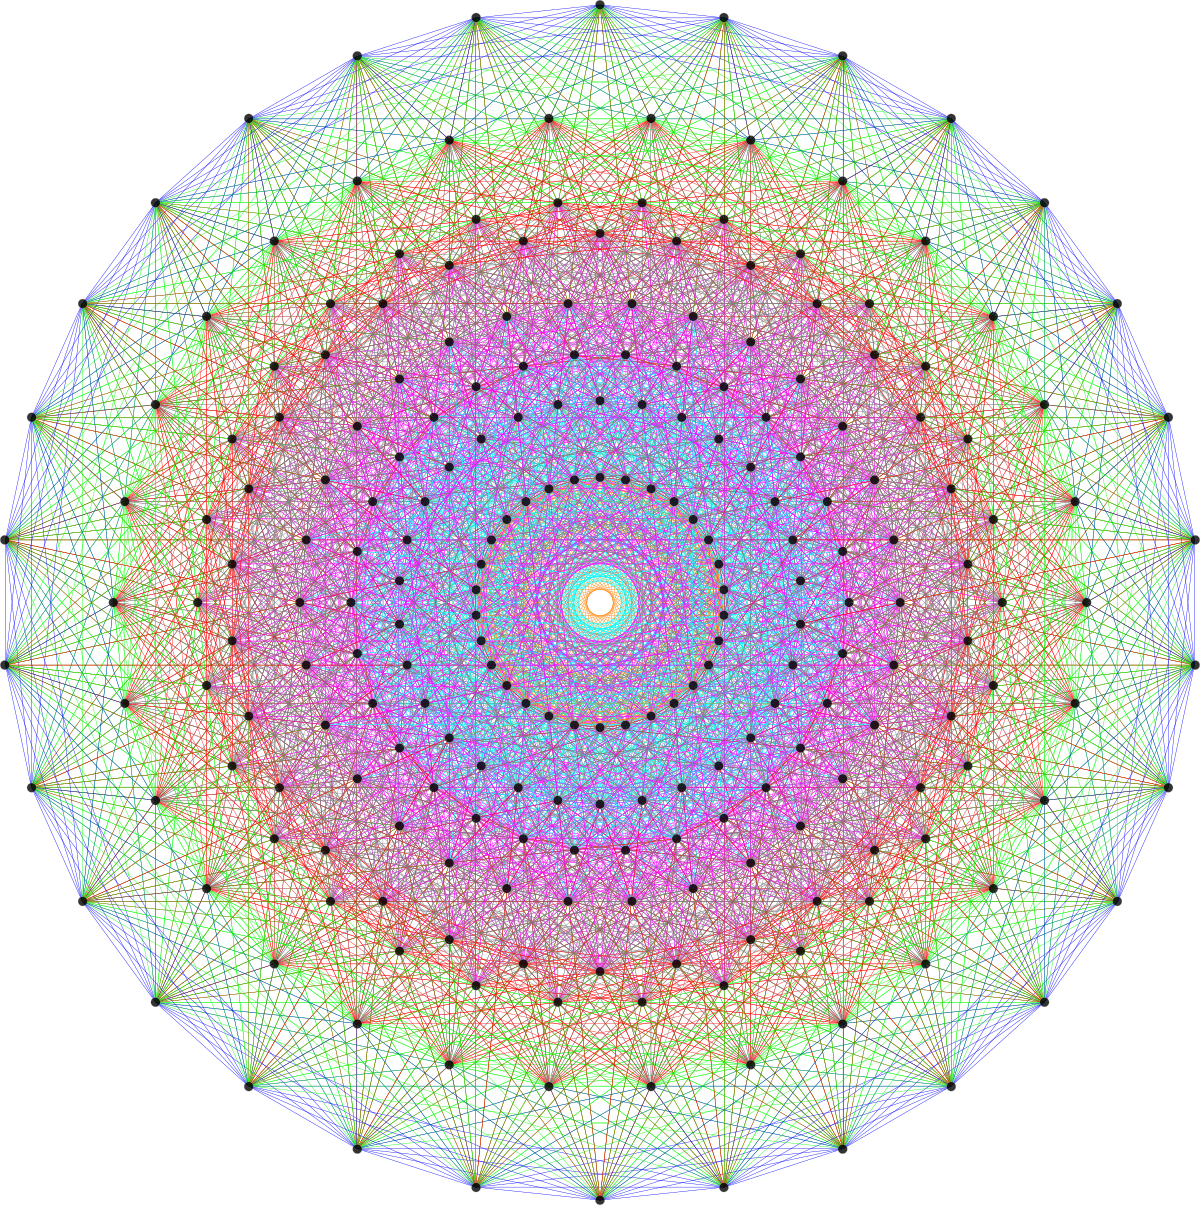
\includegraphics[scale=0.2]{E8Petrie.png}
    \caption{This \say{is} the root lattice of $E_{8}$. By that, we mean it is a projection into $2$-dimensions of the $8$ dimensional root lattice system. I'm not too sure that this picture is the right way to approach analysing $E_{8}$, but it's pretty.}
\end{figure}
\begin{remark*}\hspace{0.1cm}
    \begin{enumerate}
        \item To look up root systems, use the \say{spherical explorer} website. Link \href{http://www.liegroups.org/dissemination/spherical/explorer/cgi-bin/rootSystem.cgi}{here.}
        \item When doing computations, always helpful to compute things in terms of simple roots.
        \item The exceptional Lie algebras are written as: \begin{align*}
            \frakg_{2} & & \frakf_{4} & & \frake_{6} & & \frake_{7} & & \frake_{8}
        \end{align*}
        $\frakg_{2}$ is the algebra of \say{derivations of the octonions} $\bbO$, where a \textbf{derivation}\footnote{On Example Sheet 2, for reference} is a linear map $\delta$ such that \[ \delta(ab)=\delta(a)b + a\delta(b)\] (where multiplication is taken to be a bracket in the Lie algebra case). $\bbO$ is an $8$-dimensional normal division algebra over $\bbR$. It has a $1$ dimensional centre on which $\frakg_{2}$ acts trivially. Moreover, there is a representation \[ \frakg_{2} \to \frakso_{7} \] which is the lowest dimensional non-trivial representation of $\frakg_{2}$ (More can be found in [Humphreys, 19.3]). Other can be constructed ([Fulton and Harris, 22.4]).
        \item Given $\Phi$, there is a natural construction of a Lie algebra with that root system.
    \end{enumerate}
\end{remark*}
We've \newlec seen that there is a correspondence 
\begin{center}
    \begin{tikzcd}
        \{ \, \frakg \text{ simple, }\frakt \text{ CSA}\} \arrow[r, twoheadrightarrow] & \{ \, \text{irred root systems } \Phi\,\} \arrow[d,leftrightarrow]\\
         & \{ \, \text{connected Dynkin diagrams} \, \}
    \end{tikzcd}
\end{center}
Now we \newlec want to: \begin{itemize}
    \item Show that the root system corresponding to $\frakg$ is independent of the choice of CSA.
    \item Show that two Lie algebras with the same root system are isomorphic.
\end{itemize}
\setcounter{section}{8}
\section{Brief introduction to inner automorphisms}
Remember section 9? Here it is!
\begin{fancydefine*}{Automorphism}
    An \textbf{automorphism} of $\frakg$ is an isomorphism $\frakg \to \frakg$. The gorup of all such is $\Aut \frakg$. For example, if $\frakg = \frakgl(V)$ or $\fraksl(V)$ and $A \in \GL(V)$ is an invertible endomorphism $V \to V$, then \[ x \mapsto AxA^{-1} \] is an automorphism of $\frakg$.
\end{fancydefine*}
Take $V$ finite dimensional over $\bbC$. Take $x \in \frakg$ such that $\ad x$ is nilpotent (i.e. $(\ad x)^{m}=0$ for some $m>0$). Then \[ \exp(\ad x) = 1 + \ad x + \frac{(\ad x)^{2}}{2!} + \cdots + \frac{(\ad x)^{m-1}}{(m-1)!}\]
makes sense to define, as there are finitely many terms. It is easy to show that $\exp(\ad x) \in \Aut(\frakg)$. Any automorphism of the form $\exp(\ad x)$, where $\ad x$ is nilpotent, is called \textbf{inner}. The subgroup of $\Aut \frakg$ generated by these is denoted $\Inn \frakg$. We can see that it's normal: if $\phi \in \Aut \frakg$, $x \in \frakg$, then \[ \phi(\ad x)\phi^{-1} = \ad \phi(x).\] so we must have \[ \phi \exp(\ad x) \phi^{-1} = \exp(\ad \phi(x))\]

\begin{fancylem}{}
    If $\frakg \leq \frakgl(V)$ (over $\bbC$) and $x$ is nilpotent, then $\ad x$ is nilpotent and \[ \exp(x)y(\exp x)^{-1} = \exp(\ad x)(y) \,\,\,\, \forall y \in \frakg.\]
\end{fancylem}
\proof Humphreys, page $9$ (I think). \endproof
\begin{exs*}\hspace{0.1cm}
    \begin{enumerate}
        \item $\frakg = \fraksl_{n}(\bbC)$ : $\Inn(\frakg) = \PGL_{n}(\bbC)$.
        \item $\frakg = \frakso_{n}(\bbC)$ : $\Inn(\frakg) = \SO_{n} / Z$
        \item $\frakg = \fraksp_{2n}(\bbC)$ : $\Inn(\frakg) = \Sp_{2n}(\bbC) / Z$
    \end{enumerate}
\end{exs*}
\setcounter{section}{14}
\section{Conjugacy results}
Here $\frakg$ is a semisimple Lie algebra, $\frakt$ is a CSA of $\frakg$, $\Phi$ is a root system corresponding to $\frakt$, i.e.:
\[ \frakg = \frakt \oplus \bigoplus_{\alpha \in \Phi} \frakg_{\alpha},\] and $\Delta \subseteq \Phi$ is a root basis.
\begin{fancylem}{}
    If $\frakt'$ is another CSA of $\frakg$ then there is an inner automorphism $\Psi \in \Inn(\frakg)$ with $\Psi(\frakt) = \frakt'$.
\end{fancylem}
\proof {[}Humphreys 16.4{]} or [Carter, p34]. Pretty heavy-duty group theory. \endproof
\begin{fancydefine*}{Rank}
    Define the \textbf{rank} of $\frakg$ as the dimension of a CSA which is independent of choice of CSA by (15.1). If $\frakg$ is semisimple, then $\rank \frakg$ coincides with $\rank \Phi$,  where $\Phi$ is the root system of $\frakg$ relative to any maximal toral subalgebra (i.e. relative to any CSA).
\end{fancydefine*}

\begin{fancylem}{}
    If $\frakt'$ is a CSA of $\frakg$ with root system $\Phi$, then $\Phi$ and $\Phi'$ are isomorphic.
\end{fancylem}
\proof Take $\Psi \in \Inn \frakg$ as in (15.1), mapping $\frakt$ to $\frakt'$. Take $t \in \frakt$, $\alpha \in \Phi$, and $e_{\alpha} \in \frakg{\alpha}$. Then \[ [\Psi(t), \Psi(e_{\alpha})]=\Psi([t,e_{\alpha}])\]
since $\Psi$ is a homomorphism, so respects the bracket. Then \begin{align*}
    \Psi([t,e_{\alpha}]) &= \Psi(\alpha(t)e_{\alpha})\\
    &= \alpha(t)\Psi(e_{\alpha})
\end{align*}
Then as $\Psi(e_{\alpha})$ spans the root space for $\frakt'$, \[ \Phi' = \{ \alpha \circ \Psi^{-1} \, : \, \alpha \in \Phi\}.\] \endproof 
\begin{fancythm}{}
    Suppose $\frakg'$ is a semisimple Lie algebra with root system $\Phi$, then $\frakg \cong \frakg'$.
\end{fancythm}
\proof In [Carter, Chapter 7] using the theory of finite structure constants. The idea is to choose a basis $h_{\alpha_{i}}$ of $\frakt$, and choose $e_{\alpha}$ in each root space, so that for each $\alpha$: \[ [e_{\alpha}, e_{-\alpha}]=h_{\alpha}. \] This gives a basis of the Lie algebra. Then \begin{align*}
    [h_{\alpha_{i}},h_{\alpha_{j}}] =0, & & [h_{\alpha_{i}}, e_{\alpha}] = \alpha(h_{\alpha_{i}})e_{\alpha_{i}}, & & [e_{\alpha},e_{\beta}] = \begin{cases}
        N_{\alpha \beta} e_{\alpha + \beta}, & \alpha+\beta \in \Phi\\
        h_{\alpha}, & \beta = -\alpha\\
        0, & \alpha + \beta \notin \Phi \cup \{0\}
    \end{cases}
\end{align*}
\section{Weights}
\begin{ex*}
    Let $\frakg = \frakso_{5}(\bbC)$, this is type $B_{2}$ (which is actually the same as type $C_{2}$\footnote{Which we technically did not allow to exist when we defined these.}), $\alpha,\beta$ are simple roots for the root system of $\frakg$, which we call $\Phi$. 
    Recall, we had $\frakm_{\alpha}$ given by: \[\frakm_{\alpha} = \frakg_{\alpha} \oplus \langle [\frakg_{\alpha},\frakg_{-\alpha}] \rangle \oplus \frakg_{-\alpha} \cong \fraksl_{2}.\] 
    Decompose the adjoint representation of $\frakg$ under the actions of $\frakm_{\alpha}$, $\frakm_{\beta}$. \gap If $e_{\alpha} \in \frakg_{\alpha}$, then $e_{\alpha} \frakg_{\gamma} = \frakg_{\alpha + \gamma}$ for all $\gamma \in \Phi$. So each $\alpha$-root string corresponds to an irreducible subrepresentation ($\frakm_{\alpha}$) of $\frakg$.
     \[ \frakg|_{\frakm_{\alpha}} = V(2) \oplus V(2) \oplus V(2) \oplus V(0).\]
    Similarly: \[ \frakg|_{\frakm_{\beta}} = V(2) \oplus V(1) \oplus V(1) \oplus V(0) \oplus V(0) \oplus V(0).\]
\end{ex*}
Now $(\Phi, E)$ is a root system, and fix the base $\Delta = \{\alpha_{1}, \dots, \alpha_{l}\}$.
\begin{fancydefine}{Root lattice/Weight lattice}
    The \textbf{root lattice} $\bbZ\Phi$ is defined as \[ \bbZ\Phi = \{ \sum_{\alpha \in \Phi}c_{\alpha}\alpha, \, \, c_{\alpha} \in \bbZ\} \subseteq E.\]
    The \textbf{weight lattice} $X$ is defined: \[ X = \{ \lambda \in E, \, \, \langle \lambda, \alpha^{\checked} \rangle \in \bbZ,\,\, \forall \alpha \in \Phi\}.\] Or $\{ \beta \in \frakt^{*} \, : \, \beta(h_{\alpha}) \in \bbZ \,\, \forall \text{ roots $\alpha$}\}$.\gap The Weyl group acts on $X$
\end{fancydefine}
Note: \begin{itemize}
    \item $\bbZ\Phi \subseteq X$.
    \item If $\lambda \in X$ so is $w(\lambda)$ (since $\langle \lambda, \alpha^{\checked} \rangle = \langle w(\lambda), w(\alpha)^{\checked} \rangle)$).
    \item The root lattice \textit{is} a lattice in $E$ in the technical sense (i.e. the $\bbZ$-span of an $\bbR$-basis, i.e. it's a finitely-generated free abelian group, so isomorphic to some $\bbZ^{l}$, with form $(\widecdot, \widecdot) : L \times L \to \bbZ$, such that $(L \otimes_{\bbZ} \bbR, \, (\widecdot, \widecdot))$ is an inner product space.
\end{itemize}
\begin{fancylem}{}
    $\lambda \in X$ if and only if $\langle \lambda, \alpha^{\checked} \rangle \in \bbZ$, $\forall \alpha \in \Delta$.
\end{fancylem}
\begin{fancydefine}{Fundamental weights with respect to $\Delta$}
    For $1 \leq i \leq l$, define $\omega_{i} \in E$ by \[ \langle \omega_{i}, \alpha_{j}^{\checked} \rangle = \delta_{ij}\]
    and call $\{ \omega_{i} \}$ the \textbf{fundamental weights with respect to} $\Delta$.
\end{fancydefine}
By (16.2), \[ X= \left\{ \sum_{i} c_{i} \omega_{i} \, : \, c_{i} \in \bbZ\right\}. \]
\textbf{Exercise: }$X/\bbZ\Phi$ is a finite group, called the \textbf{fundamental group}. In fact, the index $|X/\bbZ\Phi| = \det C$ where $C$ is the Cartan matrix. [Humphreys, page 68].
\begin{ex*}
    Consider $\frakg = \fraksl_{2}$, with type $A_{1}$, and roots $\{\alpha, -\alpha\}$. The root lattice $\bbZ\Phi$ is then just $\bbZ\alpha$, and $\langle \alpha, \alpha^{\checked} \rangle = 2$, and $X = \bbZ \frac{\alpha}{2}$. Here $|X/\bbZ\Phi|=2=\det(2) = \det(C)$. In fact, for $A_{l}$, $|X/\bbZ\Phi|$ is always $l+1$. For type $B_{l}$, it's always $l$, and for $G_{2}$, $X=\bbZ\Phi$, so the index\footnote{Which we call the \say{index of connection}.} is $1$.
\end{ex*}
\begin{fancydefine}{Dominant}
    A $\lambda \in X$ is \textbf{dominant} if \[
        \langle \lambda, \alpha^{\checked} \rangle \geq 0, \, \, \forall \alpha \in \Phi^{+},\]
        \textbf{strongly dominant} if $>0$. $X^{+}$ is the set of dominant weights (sometimes called the cone of dominant weights). This is equivalent to: \begin{itemize}
            \item $\lambda$ lies in the closure of the fundamental Weyl chamber with respect to $\Delta$ (I assume this means the Weyl chamber that $\gamma$ lies in, where $\Delta = \Delta_{\gamma}$).
            \item $\lambda = \sum_{i=1}^{l} c_{i}w_{i}$ with all $c_{i} \in \bbZ_{\geq 0}$. ($X^{+} = \bigoplus_{i=1}^{l}\bbZ_{\geq 0} \omega_{i})$).
        \end{itemize} 
\end{fancydefine}
Assume $\frakg$ is semisimple, with root system $\Phi$, Cartan subalgebra $\frakt$. Choose $e_{\alpha} \in \frakg_{\alpha}$ for each $\alpha \in \Phi$, such that $[e_{\alpha},e_{-\alpha}]=h_{\alpha}$, and $\varphi: \frakg \to \frakgl(V)$ a finite dimension representation over $\bbC$.
\begin{fancylem}{Weight Space Decomposition}
    $V = \bigoplus_{\lambda \in \frakt^{*}}V_{\lambda}$ where \[V_{\lambda} = \{v \in V \, : \, tv = \lambda(t)v, \, \, \forall t \in \frakt\}\]
\end{fancylem}
\proof Clear from Lemma 10.2, where the commuting semisimple endomorphisms are the basis elements of $\frakt$. \endproof
\textbf{Some Terminology:} \gap Recall that for $\lambda, \mu \in \frakt^{*}$, we write $\mu \leq \lambda$ to mean $\lambda-\mu = \sum c_{i} \alpha_{i}$ for $\alpha_{i} \in \Delta$, and $c_{i} \in \bbZ_{\geq 0}$. \gap 
And if $V$ is a representation of $\frakg$, we say: \begin{itemize}
    \item The \textbf{weight} of vector $0 \neq v \in V$ is $\lambda$ if $v \in V_{\lambda}$.
    \item $\lambda \in \frakt^{*}$ is a highest weight if $V_{\lambda} \neq 0$ and if $V_{\mu} \neq 0$ for all $\mu \leq \lambda$ (in the above ordering).
\end{itemize}
\begin{fancyprop}{}\hspace{0.1cm}
    \begin{enumerate}
        \item If $v \in V_{\lambda}$ then $e_{\alpha}V_{\lambda} \in V_{\alpha + \lambda}$.
        \item If $V_{\lambda} \neq 0$, then $\lambda \in X$ (i.e. $\lambda(h_{\alpha}) \in \bbZ$ for all $\alpha$).
        \item $\dim V_{\lambda} = \dim V_{w\lambda}$.
    \end{enumerate}
\end{fancyprop}
\proof \hspace{0.1cm} \begin{enumerate}
    \item Fix $t \in \frakt$. Then 
        \begin{align*}
            te_{\alpha}v &= ([te_{\alpha}] + e_{\alpha}t)v\\
            &= \alpha(t)e_{\alpha}(v)+e_{\alpha}\lambda(t)v\\
            &= (\alpha + \lambda)(t)e_{\alpha}v
        \end{align*}
    \item Consider $V|_{\frakm_{\alpha}}$. Then $h_{\alpha}$ acts by integer weights, so $\lambda(h_{\alpha}) \in \bbZ$.
    \item Enough to assume $w=w_{\alpha}$ for some $\alpha \in \Phi$ (since they generate the Weyl group).\gap Now $V|_{\frakm_{\alpha}} = \bigoplus V^{(j)}$, where $V^{(j)}$ are $\frakm_{\alpha}$-irreducible representations. Since $h_{\alpha}$-weight spaces of $V^{(j)}$ are $1$-dimensional, we can choose a basis $\{v_{1},\dots, v_{n}\}$ for $V_{\lambda}$, with each $v_{i}$ in a distinct $V^{(j)}$. \gap Now it's enough to prove that given $v_{i} \in V^{(j)}, \, \exists x \in \frakm_{\alpha}$ such that $xv_{i} \in V_{w_{\alpha}\lambda}$. We know $w_{\alpha}(\lambda)=\lambda-\langle \lambda, \alpha^{\checked}\rangle \alpha$, and that $\{e_{-\alpha}^{k}v_{i}, e^{k}_{\alpha}v_{i} \, : \, k \in \bbZ_{\geq 0}\}$ spans $V^{(j)}$ (this comes from $\fraksl_{2}$-theory we developed before, i.e. jumping left and right).\gap So define \[M = \max\{k \, : \, e^{k}_{\alpha}v_{i} \neq 0\}\] and \[m = \max \{k \, : \, e^{k}_{-\alpha}v_{i} \neq 0.\] \gap We need to prove $-m \leq \langle \lambda, \alpha^{\checked} \rangle \leq M$ as in (10.13(2)). However: \[ (\lambda + M_{\alpha})(h_{\alpha}) = -(\lambda-m_{\alpha})(h_{\alpha})\] \[\therefore\, \lambda(h_{\alpha}) = m-M,\] and then since $\lambda(h_{\alpha})=\langle \lambda, \alpha^{\checked}\rangle$, we're done.
\end{enumerate}
\endproof
\begin{fancydefine}{Highest weight vector/HWV}
    $v \in V$ is a \textbf{highest weight vector} (HWV) if \begin{itemize}
        \item $v \neq 0$.
        \item $v \in V_{\lambda}$, for some $\lambda$.
        \item $e_{\alpha}(v)=0$, $\forall \alpha \in \Phi^{+}$.
    \end{itemize}
    On the example sheet, we show that there is a root $\alpha_{0}$ of maximal height with respect to $\Delta$ (the \textbf{highest root}). Any non-zero $v \in \frakg_{\alpha_{0}}$ is a highest weight vector with respect to the adjoint representation.
\end{fancydefine}
\begin{ex*}
    $\frakg = \fraksl_{3}$, $\frakt$ is the CSA, the root lattice is a series of points (which looks like a lattice of equilateral triangles, picture it) in $\bbR^{2}$, and basis for the CSA: \begin{align*}
        h_{\alpha_{1}}=\begin{pmatrix}
            1 & &\\
            & -1 &\\
            & & 0\\
        \end{pmatrix}
        & & h_{\alpha_{2}}=\begin{pmatrix}
            0 & &\\
            & 1 &\\
            & & -1\\
        \end{pmatrix}
    \end{align*}
    Let $V$ be the defining representation of $\frakg$ with standard basis $\{e_{1},e_{2},e_{3}\}$. We look for $\lambda_{i} \in \frakt^{*}$ such that $V=\bigoplus_{i}V_{\lambda_{i}}$ with basis for each $V_{\lambda_{i}}$ given by: \begin{align*}
        h_{\alpha_{1}}e_{1} = e_{1}, & & h_{\alpha_{2}}e_{2} = -e_{2} & & h_{\alpha_{1}}e_{3}=0\\
        h_{\alpha_{2}}e_{1}=0 & & h_{\alpha_{1}}e_{2}=e_{2} & & h_{\alpha_{2}}e_{3}=-e_{3}
    \end{align*}
    So let \begin{align*}
        \lambda_{1}(h_{\alpha_{1}})=1, \, \, \lambda_{1}(h_{\alpha_{2}})=0\, \Rightarrow\, V_{\lambda_{1}}=\langle e_{1} \rangle\\
        \lambda_{2}(h_{\alpha_{1}})=-1, \, \, \lambda_{2}(h_{\alpha_{2}})=1\, \Rightarrow\, V_{\lambda_{1}}=\langle e_{2} \rangle\\
        \lambda_{3}(h_{\alpha_{1}})=0, \, \, \lambda_{3}(h_{\alpha_{2}})=-1\, \Rightarrow\, V_{\lambda_{3}}=\langle e_{3} \rangle\\
    \end{align*}
    Notice $\lambda_{1} = \omega_{1}$, $\lambda_{2} = -\omega_{1} + \omega_{2}$, $\lambda_{3} = -\omega_{2}$. on the diagram on page 81. Check $e_{1}$ is a HWV ($e_{\alpha}e_{1}\in V_{\lambda + \alpha}$ etc.) [Fulton-Harris, Lectures 12,13]. 
\end{ex*}

\section{The PBW theorem}
\begin{fancylem}{}\hspace{0.1cm}
    \begin{enumerate}
        \item $V$ has HWV
        \item If $v \in\ V_{\lambda}$ is a highest weight vector, then $\lambda$ must be dominant.
    \end{enumerate}
\end{fancylem}
\proof \hspace{0.1cm}
\begin{enumerate}
    \item Choose any non-zero element $0 \neq v_{0} \in V_{\lambda}$ for some $\lambda$. If it's a HWV then we're done, otherwise, there must be a positive root $\alpha$ such that $e_{\alpha}v_{0} \neq 0$. Now let \[ k' = \max\{k \, : \, e_{\alpha}^{k}v_{0} \neq 0\}\]
    Let $v_{1} = e_{\alpha}^{k}v_{0} \in V_{\lambda+k'\alpha}$. Then repeat this argument, replacing $v_{0}$ by $v_{1}$, and keep going. This process \textit{must} end, since $V$ is finite dimensional, and each $v_{i}$ is in a distinct weight-space $V_{\mu}$, as we always add on a positive root.
    \item For $\alpha \in \Phi^{+}$, need to show $\langle \lambda, \alpha^{\checked} \rangle \in \bbZ_{\geq 0}$. Consider $\frakm_{\alpha} = \langle e_{\alpha},h_{\alpha},e_{-\alpha} \rangle$ acting on $V$. \begin{align*}
        e_{\alpha}v = 0, & & h_{\alpha}v=\lambda(h_{\alpha})v
    \end{align*}
    So $v$ is a HWV for any $\frakm_{\alpha} \cong \fraksl_{2}$ acting on $V$, hece $\lambda(h_{\alpha}) \in \bbZ_{\geq 0}$.
\end{enumerate}
\endproof
Next, we show that there is a correspondence: \[ \{\,\text{f.d. irreducible representations of $\frakg$}\,\} \leftrightarrow \{\,\text{dominant weights}\,\}\]
\large \textbf{Universal enveloping algebra}\gap  \normalsize
For now, $k$ may be any field. We associate to each Lie algebra, $\frakg$ which is defined over $k$, an associative algebra with a $1$ (infinite-dimensional in general (the algebra, not the one)) which is generated \say{as freely as possible} by $\frakg$ subject to the commutation relations in $\frakg$.
\begin{fancydefine}{}
    Let $V$ be a vector space over the base field $k$. Define the tensor algebra of $V$: \[ \scrT := k \bigoplus V \bigoplus V \otimes V \bigoplus V \otimes V \otimes V \bigoplus \cdots\]
    Or we can write this as \[ \bigoplus_{n \geq 0} V^{\otimes n} = \bigoplus_{j\geq 0} T^{j}V\] (with $T^{0}V =k$), with an associative product defined on homegeneous generators of $\scrT(V)$ by \[ v_{1} \otimes \dots v_{m} \cdot u_{1} \otimes \dots \otimes u_{n} = v_{1} \otimes \dots v_{m} \otimes u_{1} \otimes \dots \otimes u_{n}.\]
\end{fancydefine}
\begin{fancydefine*}{Symmetric algebra}
    The \textbf{symmetric algebra} on $V$ is $\Sym(V) = S(V) := \scrT(V)/I$ where $I$ is the $2$-sided ideal generated by $\{x\otimes y - y \otimes x \, : \, x,y \in V\}$. Notice that \begin{itemize}
        \item $S(V) = \bigoplus_{n \geq 0} S^{n}V$
        \item Can identify $S(V)$ with $k[V]$, the algebra of polynomials on $V$.
        \item $\scrT(V)$ and $S(V)$ are graded rings.
    \end{itemize}
\end{fancydefine*}
\begin{fancydefine}{Universal enveloping algebra}
    Given an arbitrary Lie algebra $\frakg$ (really arbitrary, possibly infinite dimensional), then the \textbf{universal enveloping algebra} $\scrU(\frakg)$ is the associative $k$-algebra \[ \scrT(\frakg)/J\] where $J$ is the $2$-sided ideal generated by \[ \{x\otimes y - y \otimes x - [x,y] \, : \, x,y \in \frakg\}\]
\end{fancydefine}
\textbf{Some facts/exercises:} \begin{itemize}
    \item We often write $x \otimes y$ as $xy$
    \item If $V$ is a representation of $\frakg$, then $V$ is a $\scrU(\frakg)$-module: \[ (x_{1} \otimes \dots x_{n})v = x_{1}(\dots x_{n}(v)).\] This is well-defined, because $(x \otimes y - y\otimes x)v$ = $(xy-yx)v = [x,y]v$.
    \item If $V$ is a finite dimensional $\bbC$-representation of $\frakg$, i.e. $\fraksl_{2}$, recall that we defined the Casimir element \[ \Omega = ef + fe + \frac{1}{2}h^{2} \in \frakgl(V).\] $\Omega$ is naturally an element of $\scrU(\frakg)$, independent of $V$. In general, if $\frakg$ is a semisimple complex Lie algebra, with basis $\{x_{1},\dots, x_{n}\}$, then let $\{y_{1},\dots,y_{n}\}$ be the dual basis with respect to the Killing form. Then \[\Omega = \sum_{i=1}^{n} x_{i}y_{i}\] which is in $\scrU(\frakg)$ by making the appropriate identifications. This is the Casimir element of (7.19). It's central in $\scrU(\frakg)$, just as it was central in $\fraksl_{2}$.
    \item $\scrU(\frakg)$ is not graded, e.g. $\frakg \otimes \frakg$ is not closed under addition. For example \[
        x \otimes y - y \otimes x -[x,y]
        \] is not homogeneous, but is equal to $0$. But it \textit{does} have a filtration: Let \[ U_{n} = \text{ image of } \bigoplus_{i=0}^{n} \frakg^{\otimes i}\] in $scrU(\frakg)$. Then $U_{n}U_{m}\subseteq U_{n+m}$. \gap \textbf{Exercise: }If $x \in U_{n}$ and $y \in U_{m}$, then $xy-yx \in U_{m+n-1}$. Write \[ x= \sum_{i=1}^{p}\lambda_{i}x_{1}^{i} \dots x_{n}^{i}, \, \, y=\sum_{j=1}^{q}\mu_{j}y_{1}^{j} \dots y_{m}^{j}\]
\end{itemize}
\begin{fancydefine}{Graded algebra associated to a filtration}
    Given any filtration \[\calF_{0} \subseteq \calF_{1} \subseteq \dots, \] call $\gr \calF = \oplus_{i} \calF_{i}/ \calF_{i-1}$ the \textbf{associated graded algebra}. In our case \[ \gr \scrU(\frakg) = U_{0} \oplus (\bigoplus_{n \geq 1} U_{n}/U_{n-1}).\]
\end{fancydefine}
\begin{fancythm}{PBW Theorem}
    There is an algebra isomorphism \begin{enumerate}
        \item $S(\frakg) \xrightarrow{\sim} \gr(\scrU(\frakg))$
        \item Equivalently, if $\{x_{1}, \dots, x_{n}\}$ is a basis for $\frakg$, then \[ \{x_{1}^{k_{1}},\dots,x_{n}^{k_{n}} \, : \, k_{i} \in \bbZ_{\geq 0}\}\] is a basis for the universal enveloping algebra $\scrU(\frakg)$. In particular $\frakg \hookrightarrow \scrU(\frakg)$.
    \end{enumerate}
\end{fancythm}
\proof Quite involved. Statement $1$ is done in [Humphreys, 17.4]. The sketch is that, we have a map \[ \frakg \xrightarrow{\iota}U_{n} \xrightarrow{/U_{n-1}} U_{n}/U_{n-1}\] which gives a map from the tensor algebra to the associated graded algebra, which (by the exercise just before proposition 17.4) factors through the symmetric algebra $S(\frakg)$. So we have a commutative diagram\footnote{as every Part III course must have.}: \begin{center}
    \begin{tikzcd}
        \scrT(\frakg) \arrow[rd] \arrow[r] & \gr(\scrU)\\
        & S(\frakg) \arrow[u]\\
    \end{tikzcd}
\end{center}
This map is surjective (which is not hard to show). It remains to show that the map is injective (which \textit{is} hard to show).\gap 
To prove $2$, we have a basis for $S(\frakg)$, which gives a basis for $\gr(\scrU)$. And this, in turn, gives a basis for $\scrU(\frakg)$. This is proved in [Humphreys, 17.3, Corollary C]. \endproof
\begin{fancylem}{}
    Suppose $V$ is a representation of $\frakg$ and $v \in V$. Then the minimal subrepresentation of $V$ which contains $v$ is \[ \scrU(\frakg)v = \{ uv : u \in \scrU(\frakg)\}.  \]
\end{fancylem}
\proof $\scrU(\frakg)v$ contains: \begin{itemize}
    \item The elements $x_{i}v$ $\forall x_{i} \in \frakg$.
    \item The scalar multiples of the above.
    \item The sums of the above.
\end{itemize}
\endproof
\begin{ex*}
    Let $V$ be a $\bbC$-space, with basis $\{v_{0}, \dots, v_{n}\}$. Define an $\fraksl_{2}$-action on $V$ by: \begin{align*}
        e.v_{0}=0, & & h.v_{0} = 0, & & f.v_{i}=v_{i+1}.
    \end{align*}
    Then we claim that $v_{0}$ and $v_{1}$ are HWVs for the $\fraksl_{2}$-action. So we require \[ ev_{j} = 0 \,\,\,\,\,\, \, \, j=0,1\]
    When $j=0$ this is done by assumption. \gap When $j=1$, we have \begin{align*}
        ev_{1} &= efv_{0}\\
               &= ([ef] +fe)v_{0}\\
               &= [ef]v_{0}\\
               &= hv_{0}\\
               &=0
    \end{align*}
    We also require that $\langle v_{0} \rangle$ and $\langle v_{1} \rangle$ require their own images under $h$ (the weight-space condition for HWVs). \gap 
    For $v_{0}$ this is done, since it is clear. \gap 
    For $v_{1}$: \begin{align*}
        hv_{1} &= hfv_{0}\\
               &= ([hf] +fh)v_{0}\\
               &= [hf]v_{0}
               &= -2fv_{0}
               &= -2v_{1}
    \end{align*}
    so $v_{1} \in V_{-2}$ is a HWV.
    Also note that \[ \langle v_{1},v_{2}, \dots, v_{n} \rangle \cong W\] is a subrepresentation of $V$, and $V/W \cong V(0)$. Since it is a 1-dimensional representation. More generally, if $V^{(n)}$ is a space with basis $\{v_{0}, v_{1}\dots\}$ with $\fraksl_{2}$ action given by \begin{align*}
        ev_{0}=0, & & hv_{0} = nv_{0}, & & fv_{i}=v_{i+1}.
    \end{align*}
    then $v_{n+1}$ is a HWV, and $W_{n} = \langle v_{n+1}, v_{n+2}, \dots \rangle$ has $V^{(n)}/W_{n} \cong V(n)$.
\end{ex*}
\section{Highest weight and Verma modules}
In this chapter, we take $\frakg$ a Lie algebra, $\frakt$ a CSA, $\Phi$ the set of roots of $\frakg$ with respect to $\frakt$, and $\Delta = \{ \alpha_{1}, \dots, \alpha_{l}\}$  root basis. If $V$ is a representation of $\frakg$, then \[ V_{\lambda} = \{v \in V \, : \, tv = \lambda(t)v \, \, \forall t \in \frakt\},\] as in (16.5).
\begin{remark*}\hspace{0.1cm}
    \begin{enumerate}
        \item $V_{\lambda}$ makes sense even if $V$ is infinite dimensional.
        \item The definition of HWV also makes sense if $V$ is infinite dimensional.
        \item If $e_{\alpha} \in \frakg_{\alpha}$ is non-zero, then $e_{\alpha}V_{\lambda} \subseteq V_{\lambda+\alpha}$ (even if $V$ is infinite-dimensional).
    \end{enumerate}
\end{remark*}
\begin{fancydefine}{Highest weight module}
    A representation $V$ of $\frakg$ is a \textbf{highest weight module} if $V$ contains a HWV, $v$, such that $V=\scrU(\frakg)v$.
\end{fancydefine}
\begin{exs}\hspace{0.1cm}
    \begin{itemize}
        \item Any finite dimensional irreducible representation $V$ of $\frakg$ is a highest weight module, since $V$ must contain a highest weight vector $v$ (17.1), and (17.6) implies that $\scrU(\frakg)$ is a subrepresentation of $V$, therefore $\scrU(\frakg) = V$ since $V$ is irreducible.
        \item In the above example, (end of \textsection 17), $v_{0}$ is a highest weight vector, $v_{i} = f^{i}v_{0}$, $V= \scrU(\frakg)v_{0}$ is a highest weight module.
    \end{itemize}
\end{exs}
\begin{remark*}\hspace{0.1cm}
    \begin{enumerate}
        \item Not every highest weight module is irreducible.
        \item If $V$ is an infinite dimensional highest weight module, and $v \in V_{\lambda}$ a HWV, $\lambda$ is not necessarily dominant (recall that it is dominant in the finite dimensional case ((17.1)2).)
    \end{enumerate}
\end{remark*}
\textbf{Notation:} \gap 
We will use $\eta^{+}$ to denote \[ \eta^{+} = \sum_{\alpha \in \Phi^{+}} \frakg_{\alpha},\] and $\eta^{-}$ to denote \[ \eta^{+} \sum_{\alpha \in \Phi^{-}} \frakg_{\alpha}.\] So we have \[ \frakg = \eta^{+} \oplus \frakt \oplus \eta^{-}.\]
\begin{fancylem}{}
    Suppose $V$ is a highest weight module with HWV $v$ such that $V=\scrU(\frakg)v$. Then $V = \scrU(\eta^{-})v$.
\end{fancylem}
\proof Choose a basis $\{x_{1}, \dots x_{n}\}$ of $\eta^{-}$, a basis $\{t_{1}, \dots, t_{l}\}$ of $\frakt$, and $\{y_{1}, \dots, y_{n}\}$ of $\eta^{+}$. Then \[ \scrU(\frakg) = \scrU(\eta^{-}) \oplus \scrU(\frakt) \oplus \scrU(\eta^{+}),\] and \[\scrU(\frakg)v = \langle x_{1}^{k_{1}}\dots x_{n}^{k_{n}}t_{1}^{m_{1}},\dots t_{l}^{k_{l}}y_{1}^{r_{1}}\dots y_{n}^{r_{n}}\rangle\]
But $y_{i}v=0$ for all $i$, and $t_{i}v = \langle v \rangle$. Therefore \[ \scrU(\frakg)v = \scrU(\eta^{-})v.\]
\begin{fancyprop}{}
    Let $V$ be a highest weight module with highest weight vector given by $v_{\lambda} \in V_{\lambda}$ such that $V = \scrU(\frakg)v_{\lambda}$. Then \begin{enumerate}
        \item $V = \bigoplus_{\mu \in D(\lambda)} V_{\mu}$ where $D(\lambda) = \{ \lambda - \sum_{i=1}^{l} k_{i}\alpha_{i} \, : \, k_{i} \in \bbZ_{\geq 0}\}$, where $\alpha_{i} \in \Delta$.
        \item Any submodule of $V$ is a direct sum of weight spaces.
        \item The dimension, $\dim V_{\lambda} = 1$, and any other $V_{\mu}$ is finite dimensional.
        \item $V$ is irreducible iff every HWV lies in $V_{\lambda}.$
        \item $V$ contains some maximal (proper) subrepresentation.
    \end{enumerate}
\end{fancyprop}
\proof \hspace{0.1cm}
\begin{enumerate}
    \item By the PBW theorem, we can write $V = \scrU(\eta^{-})v_{\lambda}$, therefore take expressions of the form  \[e_{-\beta_{2}} e_{-\beta_{2}} \dots e_{-\beta_{r}} v_{\lambda}\] where $\beta_{i} \in \Phi^{+}, \, r \in \bbZ_{\geq 0}$ and $e_{-\beta_{i}} \in \frakg_{-\beta_{i}}$. Expressions of this form span $V$. The weight of such an expression is $\lambda - \beta_{1} - \dots - \beta_{r}$, so the generators live in $V_{\lambda-\sum \beta_{i}}$ where ($\beta_{i} \in \Phi^{+})$. So (1) and also (3) must hold, as given some $\mu$, there exists only a finite number of ways to write $\mu$ as $\lambda - \sum \beta_{i}$ for $\beta_{i} \in \Phi^{+}$.
    \item Let $W$ be a submodule of $V$. Write $w \in W$ as a sum of vectors $v_{i} \in V_{\mu_{i}}$, each belonging to distinct weight spaces. We need to show that all of the $v_{i}$ lie in $W$. Suppose they don't. Then we can choose a $w$ such that \[ w = \sum_{k=1}^{n}v_{k} \] with $n$ minimal, $n>1$. In particular, no $v_{i}$ belongs to $W$. Find $t \in \frakt$ such that $\mu_{1}(t) \neq \mu_{2}(t)$. Then  \[ tw = \sum \mu_{i}(t)v_{i} \in W.\] Then also \[(t-\mu_{1}(t).1)w = (\mu_{2}(t)-\mu_{1}(t))v_{2} + \cdots + (\mu_{n}(t)-\mu_{1}(t))v_{n} \in W.\] By the choice of $w$ with $n$ minimal forces $v_{2} \in W$.
    \item[4.] Suppose that $V$ has HWV $v_{\mu} \in V_{\mu}$ where $\mu \neq \lambda$. Then $\scrU(\frakg)v_{\mu}$ is a subrepresentation of $V$, and $v_{\lambda} \notin \scrU(\frakg)v_{\mu}$. (Reason: weights for $\scrU(\frakg)v_{\mu}$ are of the form $\mu- \sum k_{i}\alpha_{i}$ for $k_{i} \in \bbZ_{\geq 0}$, so in particular, $\scrU(\frakg)v_{\mu}$ is a non-trivial proper subrepresentation). \gap 
    Conversely, suppose we can find $U \subseteq V$ a proper subrepresentation of $V$, then by (2), we can write $U$ as a direct sum of weight spaces, $V_{\mu}$. Choose $\mu$ to be such that $\mu = \lambda - \sum k_{i} \alpha_{i}$ where, as usual $k_{i} \in \bbZ_{\geq 0}$ such that $v_{\mu} \in U$ and $\sum k_{i}$ is minimal. Let $v_{\mu} \in V_{\mu}$ be non-zero, $\alpha \in \Phi^{+}$, and $e_{\alpha} \in \frakg_{\alpha}$. Then \[ e_{\alpha}v_{\mu} \in V_{\mu + \alpha} \cap U = 0,\] by the choice of $U$. Hence $v_{\mu}$ is a HWV for $V$
    \item[5.] Left as exercise. Take a proper submodule, which lies in the sum of the weight spaces other than $\lambda$, and take then sum of all such submodules, and this is proper. (In notes).
\end{enumerate}
\endproof
\textbf{Exercises: }\begin{enumerate}
    \item Show that $V$ is indecomposable (as a $\frakg$-module).
    \item Show every non-zero homomorphic image of $V$ is also a HWM.
\end{enumerate}
\subsection{Towards Verma Modules!}
Let $\Phi$, $\alpha \in \Delta$, $\lambda$ is dominant., then $\lambda - \alpha$ is also dominant. In particular, $(\lambda-\alpha, \lambda - \alpha) \leq(\lambda, \lambda)$, \begin{align*}
    (\lambda - \alpha, \lambda - \alpha) &= (\lambda, \lambda) - (\alpha, \lambda) - (\lambda - \alpha, \alpha).\\
    &= (\lambda, \lambda) - \text{something positive}
\end{align*}
which can be determined as a result of the fact that $\lambda$ is dominant. \begin{fancydefine}{highest weight of a HWM}
    If $V$ is a HWM with $v \in V_{\lambda}$ and $V = \scrU(\frakg)v$, where $v$ is a HWV, we say that $V$ is of \textbf{highest weight} $\lambda$.
\end{fancydefine}
Let $\frakt$ be a CSA of $\frakg$, $\Phi$ the corresponding root system, $\Delta$ a base, $\Phi^{+}$ the set of positive roots w.r.t. $\Delta$. Choose basis $h_{1}, \dots, h_{l}$ of $\frakt$ such that $h_{i} = h_{\alpha_{i}}$ for $\alpha_{i} \in \Delta$. For $\lambda \in \frakt^{*}$, let $J(\lambda)$ be a left-ideal of the universal enveloping algebra $\scrU(\frakg)$ generated by $e_{\alpha}$ for $\alpha \in \Phi^{+}$, and also combinations $h_{i} - \lambda(h_{i})\cdot 1$ for $1 \leq i \leq l$. I.e. $J(\lambda)$ comprises elements \[ \sum u_{\alpha} e_{\alpha} + \sum y_{i}(h_{i} - \lambda(h_{i}) \cdot 1)\] where $u_{\alpha}, y_{i} \in \scrU(\frakg)$. $J(\lambda)$ is a left-module for $\scrU(\frakg)$.
\begin{fancydefine}{Verma Module associated to $\lambda$}
    Let $M(\lambda)$ be given as \[ M(\lambda) := \scrU(\frakg) / J(\lambda)\]
    Then $M(\lambda)$ is a $\scrU(\frakg)$-module with action $u \cdot (v + J(\lambda)) = u\cdot v + J(\lambda)$. We say that $M(\lambda)$ is the \textbf{Verma Module associated to} $\lambda \in \frakt^{*}$.
\end{fancydefine}
\begin{fancyprop}{} \hspace{0.1cm}
    \begin{enumerate}
        \item This is HWM of highest weight $\lambda$.
        \item $M(\lambda)$ is \say{universal} meaning that if $m_{\lambda} \in M(\lambda)_{\lambda}$ is a HWV and $V$ is a HWM of highest weight $\lambda$, and highest weight vector $v_{\lambda} \in V_{\lambda}$ then there exists a unique $\frakg$-equivariant linear map: \begin{align*}
            M(\lambda) &\to V\\
            m_{\lambda}&\mapsto v_{\lambda}
        \end{align*}
    \end{enumerate}
\end{fancyprop}
\proof \hspace{0.1cm}
\begin{enumerate}
    \item Let $m_{\lambda} = 1+ J(\lambda) \in M(\lambda)$ (a generator as a $\scrU(\frakg)$-module). Then \[ h_{i}m_{\lambda} = h_{i} + J(\lambda) = \lambda(h_{i}) \cdot 1 + J(\lambda) \] since $h_{i} - \lambda(h_{i}) \in J(\lambda)$. \gap And if $\alpha \in \Phi^{+}$ and $e_{\alpha} \in \frakg_{\alpha}$, then $e_{\alpha}m_{\lambda} = e_{\alpha} + J(\lambda) = J(\lambda) = 0 + J(\lambda) \in M(\lambda)$, and $m_{\lambda}$ is a HWV of weight $\lambda$, since it is annihilated by $e_{\alpha}$. Clearly $M(\lambda) = \scrU(\frakg)m_{\lambda}$, so any other HWV is a scalar multiple of this one (18.4).
    \item By PBW theorem, if $\Phi^{+} = \{\beta_{1}, \dots, \beta_{r}\}$, then $e_{-\beta_{1}}\cdots e_{-\beta_{r}} \cdot m_{\lambda} \,\,\, (r \in \bbZ_{\geq 0})$, is a basis for $M(\lambda)$. Define \begin{align*}
        \varphi: M(\lambda) &\to V\\
        e_{-\beta_{1}} \cdots e_{-\beta_{r}} \cdot m_{\lambda} &\mapsto e_{-\beta_{1}} \cdots e_{-\beta_{r}} v_{\lambda}
    \end{align*}
    and check that this is $\frakg$-equivariant.
\end{enumerate}
\begin{fancylem}{}
    Given $\lambda \in \frakt^{*}$, there is a unique irreducible highest weight module with highest weight $\lambda$, call it $V(\lambda)$.
\end{fancylem}
\proof You know that $M(\lambda)$ has unique maximal (proper) submodule (by 18.4) called $J$. Then $M(\lambda)/J$ is irreducible. Uniqueness comes from the universal property. \endproof
\begin{exs*}\hspace{0.1cm}
    \begin{enumerate}
        \item In the example at the end of $\S 17$, $V=M(0)$, $J= \langle v_{1}, v_{2}, \dots \rangle$, $M(0)/J \cong V(0)$, the trivial $\fraksl_{2}$-representation.
        \item {[}EW, Ex 15.12{]} give an example of irreducible Verma modules for $\frakg= \fraksl_{2}(\bbC)$. This shows $\frakg$ has infinite-dimensional irreducible representations.
    \end{enumerate}
\end{exs*}
\begin{remark*}\hspace{0.1cm}
    \begin{enumerate}
        \item Verma modules are building blocks for \say{Category $\scrO$.} Although each $M(\lambda)$ is infinite-dimensional, when viewed as $\scrU(\frakg)$-modules, they have \say{finite length,} i.e. there are submodules \[ 0 \subseteq M_{0} \subseteq M_{1} \subseteq \cdots \subseteq M_{r} = M(\lambda)\] such that $M_{i}/M_{i-1}$ are irreducible.
        \item In 1985 Drinfield and Jimbo (independently) defined \textbf{quantum groups} by \say{deforming} the universal enveloping algebras of Lie algebras. They have numerous applications in theoretical physics, knot theory, and the representation theory of algebraic groups.
    \end{enumerate}
\end{remark*}
\begin{fancythm}{}
    $V = V(\lambda)$ is a finite dimensional, irreducible $\frakg$-module if and only if $\lambda \in X^{+}$.
\end{fancythm}
\proof \hspace{0.1cm}
\begin{enumerate}
    \item[($\Rightarrow$)] If $V$ is finite dimensional, then for each simple root $\alpha_{i}$, let $\frakm_{\alpha_{i}}$ be the corresponding copy of $\fraksl_{2}(\bbC)$ in $\frakg$. Then $V$ is also a finite dimensional module for $\frakm_{\alpha_{i}}$, and a HWV for $\frakg$ is also a HWV for $\frakm_{\alpha_{i}}$. In particular, since there is a highest weight vector of weight $\lambda$, the wight for the CSA $A_{i} \subseteq \frakm_{\alpha_{i}}$ is determined by $\lambda(h_{i})$ since \[ h_{\alpha_{i}}v :=h_{i}(v)=\lambda(h_{i})v = \langle \lambda, \alpha_{i}^{\checked} \rangle v \]
    This forces $\lambda(h_{i}) \in \bbZ_{\geq 0}$.
    \item[($\Leftarrow$)] $V(\lambda)$ is a direct sum of finite dimensional weight spaces (since $M(\lambda)$ is). The idea is to show that $\Pi (\lambda) = \{ \mu : V(\lambda)_{\mu} \neq 0 \} $ (a set of weights) is finite.\gap Have $\Delta = \{ \alpha_{1}, \dots, \alpha_{l} \}$ a set of simple roots. For each $i$, $\{x_{i}, y_{i}, h_{i}\}$ is an $\frakm_{\alpha_{i}}$-triple. We need that, for $k \geq 0$ (in $\scrU(\frakg)$): \begin{enumerate}
        \item[(i)] $[x_{j}, y_{i}^{k+1}]=0$ for $i \neq j$
        \item[(ii)] $[x_{i}, y_{i}^{k+1}] = -(k+1)y_{i}^{k} (k \cdot 1 - h_{i})$.
    \end{enumerate}
    these are proved in [Humphreys, 21.2]
    \begin{enumerate}
    \item[1.] First of all, we show that $V(\lambda)$ contains a non-zero, finite dimensional $\frakm_{\alpha_{i}}$-module for each $i$.\gap 
    Let $v$ be a HWV in $V(\lambda)$. As $\lambda \in X^{+}$, $n_{i} = \langle \lambda, \alpha_{i}^{\checked} \rangle = \lambda(h_{i}) \in \bbZ_{\geq 0}$. Then we claim $u = y_{i}^{n_{i}+1}v = 0$. 
    \gap Claim (i) above implies that \[x_{j}u= y_{i}^{n_{i}+1}(x_{j}v) + [x_{j}y_{i}^{n_{i}+1}] = 0\] for $(i \neq j)$. \gap And claim (ii) above implies that \[x{i}u =y_{i}^{n_{i}+1}(x_{i}v) + [x_{i}y_{i}^{n_{i}+1}]v = -(n_{i} + 1)y_{i}^{n_{i}}(n_{i}-h_{i})v = 0,\] as $h_{i}v = n_{i}v$.\gap  
    If $u \neq 0$, $u$ would be a HWV of weight $\lambda - (n_{i} + 1)\alpha_{i} < \lambda$. Contradiction, as highest weight is unique, so \[W = \langle v, y_{i}v, \dots, y_{i}^{n_{i}+1}v \rangle\] is a non-zero finite dimensional $\frakm_{\alpha_{i}}$-subrepresentation of $V(\lambda)$. \gap {[}Check: $h_{i}W \subseteq W$, $y_{i}W \subseteq W$ clear, $x_{i}W \subseteq W$ needs (i) above.{]}
    \item[2.] For each $i$, $V(\lambda)$ is the sum of all finite-dimensional $\frakm_{\alpha_{i}}$-subrepresentations contained in it. \gap Let $W$ = sum of all finite dimensional $\frakm_{\alpha_{i}}$-modules contained in $V(\lambda)$. Show $W$ i a $\frakg$-submodule of $V(\lambda)$. With (1) (says $W \neq 0$), this forces $W = V(\lambda)$. For $x \in \frakg$, $w \in W$, need $xw \in W$. Since $w \in W$, we must have $ w \in W'$ for some finite dimensional $\frakm_{\alpha_{i}}$module $W'$.
    Let $x' = \sum_{\beta \in \Phi \cup \{0\}} x_{\beta}$, $x_{\beta} \in \frakg_{\beta}$, then $xw \in \spann_{\beta}\{x_{\beta} W'\} = W''$. $W''$ is finite dimensional, and clearly it is $\frakm_{\alpha_{i}}$-invariant ($x_{i}W'' \subseteq \spann_{\beta}\{x_{i}x_{\beta}W'\}$), and so \[x_{i}x_{\beta}W' = x_{\beta}(x_{i}W') + [x_{i},x_{\beta}]W' \subseteq x_{\beta} W' + \frakg_{\alpha_{i} + \beta} W' \subseteq W'' \]
    Similarly, repeat for $y_{i}$, $h_{i}$. So \[ xw \in W'' \subseteq W.\] Now show Weyl group acts on $\Pi (\lambda)$ by permutations. If so, then $\Pi (\lambda)$ decomposes as disjoint union of Weyl-orbits. This will mean it's enough to show there are only finitely many orbits: use this together with the fact that the Weyl group is finite to get $\Pi (\lambda)$ finite. 
    \item[3.] $\mu \in \Pi (\lambda) \Rightarrow w_{i} \mu \in \Pi(\lambda)$, where $w_{i}$ is the reflection corresponding to $\alpha_{i}$.
    Also $\dim V(\lambda)_{\mu} = \dim V(\lambda)_{w_{i}\mu}$. Since $V(\lambda)_\mu$ is finite dimensional, there is, by (2), a finite dimensional $\frakm_{\alpha_{i}}$-module $U$ containing $V(\lambda)_\mu$. \gap For \newlec $0 \neq w \in V(\lambda)_\mu$, we have $h_{\alpha_{i}}w := h_{i}w = \mu(h_{i})w$. But $w \in U$ is then a weight vector for $h_{i}$, so by $\fraksl_{2}$-theory, \[\mu(h_{i}) = \langle \mu, \alpha_{i}^{\checked} \rangle = \text{an integer, $m$}.\] Therefore all weights are in $\bbZ$, as this holds for all $i$. As $m$ occurs as a weight of $U$, so must $-m$, and $\dim U_{m} = \dim U_{-m}$. \gap If $m \in \bbZ_{\geq 0}$, then $y_{i}^{m}w \neq 0$, and lives in $U_{-m}$. But, \[y_{i}^{m}w \in V(\lambda)_{\mu - \langle \mu, \alpha_{i}^{\checked} \rangle \alpha_{i}}\]
    because \say{weights add}, that is to say, $w_{i}\mu$ is also a weight. If $m \in \bbZ_{<0}$ just take $x_{i}^{-m}w$, and apply the same argument. \gap Now we need to show that the dimensions are equal. Suppose that $\{w_{1}, \dots, w_{r}\}$ is a basis of $V(\lambda)_{\mu}$, then $\{w_{1}, \dots, w_{r}\}$ is linearly independent in $U_{m}$. Therefore, applying $y_{i}^{m}$ or $x_{i}^{-m}$ as appropriate leaves the vectors linearly independent, and sends them to $V_{\mu - \langle \mu, \alpha_{i}^{\checked}\rangle \alpha_{i}} = V_{w_{i}\mu}$. So \[ \dim V(\lambda)_\mu \leq \dim V(\lambda) w_{i}\mu. \]
    Applying the same procedure to $w_{i}\mu$ gives \[ \dim V(\lambda)_{w_{i}\mu} \leq \dim V(\lambda)_{w_{i}^{2}\mu}.\] But $w_{i}$ is a reflection, so $w_{i}^{2}=e$.
    \item[4.] For $\mu \in \Pi(\lambda)$, its Weyl orbit\footnote{The orbit of the Weyl group acting on $\mu$.} $W\mu$ contains a dominant weight. \gap $W\mu$ is finite, therefore we can choose $\eta \in W\mu$ maximal with respect to $\leq$. Then $\eta$ must be dominant, since supposing it weren't, we would have \[ \langle \eta, \alpha_{i}^{\checked} \in \bbZ_{< 0}\rangle \] for some $i$. Then $w_{i}\eta \in W\mu$, $w_{i}\eta = \eta - \langle \eta, \alpha_{i}^{\checked} \rangle \alpha_{i} > \eta$, contradiction to the chocie of $\eta$.
    \item[5.] The set $S = \{ \eta : \eta \text{ dominant, } \eta \leq \lambda \}$ is finite.\gap If $\eta \in S$, then $\lambda - \mu = \text{ sum of positive roots with $\bbZ_{\geq 0}$ coefficients}.$ Hence $\eta$ lies in a discrete set. Also $\lambda + \eta$ is dominant, therefore \[ \langle \lambda + \eta, \alpha_{i}^{\checked}\rangle \geq 0 \,\,\,\, \forall i,\] in particular \[ (\lambda+\eta,\lambda-\eta) \geq 0 \Rightarrow (\lambda, \lambda) \geq (\eta, \eta),\]
    So $\eta$ lies in a compact set, since it is in the closed ball of radius $\sqrt{(\lambda,\lambda)}$. Compact and discrete means finite, so $S$ must be finite.
    \end{enumerate}
    From (4), any $W$-orbit of $\Pi(\lambda)$ contains an element of $S$, and (5) implies that the number of orbits is finite.
\end{enumerate}
\endproof
So there is a bijection \[ \{\, \text{dominant weights, $\lambda$}\,\} \leftrightarrow \{\text{f.d. irred representations $V(\lambda)$ of $\frakg$}.\}\] 
\section{The Weyl character formula}
Let $\frakg$ be a semisimple Lie algebra, $\frakt$ a CSA, $\Delta = \{\alpha_{1}, \dots, \alpha_{l}\} \subseteq \Phi$ a choice of root basis inside the set of roots, $X$ the weight lattice, $W$ is the Weyl group.
\begin{ex*}
    Define \[ \rho = \frac{1}{2} \sum_{\alpha \in \Phi^{+}} \alpha.\] Compute $\langle \rho, \alpha_{i}^{\checked} \rangle$ for each $\alpha_{i} \in \Delta$ in types $A_{1}, A_{2},$ and $B_{2}$. For $A_{2}, B_{2}$, we can write $\Delta = \{ \alpha_{1}, \alpha_{2} \}$. Then we claim that $\rho = \omega_{1} + \omega_{2}$: \begin{itemize}
        \item $A_{1}$: $\{\alpha_{1}, -\alpha_{1}\}$, $\rho = \frac{\alpha}{2}$, $\langle \rho, \alpha^{\checked} \rangle = 1$.
        \item $A_{2}$: $\langle \rho, \alpha_{1}^{\checked} \rangle = \langle \omega_{1} + \omega_{2}, \alpha_{1}^{\checked} \rangle = 1$
        \item $B_{2}$: $\langle \rho, \alpha_{i}^{\checked} \rangle = 1$.
    \end{itemize}
    Then the claim is that $\rho = \sum_{i=1}^{l}\omega_{i}$ ( $\omega_{i}$ as defined in (16.3)). \gap 
    It is enough to show that $\langle \rho, \alpha_{j}^{\checked} \rangle  = 1$ for all $\alpha_{j} \in \Delta$. Now \[ w_{\alpha_{j}}(\rho) = \rho - \langle \rho, \alpha_{j}^{\checked} \rangle \alpha_{j},\] and also \[ w_{\alpha_{j}}(\rho) = w_{\alpha_{j}}\left( \frac{1}{2} \left( \sum_{\alpha \in \Phi^{+}\setminus \{\alpha_{j} \}} \alpha \right) + \frac{1}{2}\alpha_{j}\right),\]
    and $w_{\alpha_{j}}$ permutes $\Phi^{+}\setminus \{ \alpha_{j} \}$, so this is \[ \frac{1}{2} \left( \sum_{\alpha \in \Phi^{+} \setminus \{ \alpha_{j} \} } \right) - \frac{1}{2}\alpha_{j} = \rho - \alpha_{j}.\]
    Comparing the two expressions, $\langle \rho , \alpha_{j}^{\checked} \rangle = 1$. 
\end{ex*}
Recall from (18.9) that $\Pi(\lambda) = \{ \mu : V(\lambda)_{\mu} \neq 0 \}$. Possible questions: \begin{itemize}
    \item What is $\Pi(\lambda)$?
    \item What is $\dim V(\lambda)$?
\end{itemize} 
\begin{fancydefine}{Ordering on $X$}
    Partial ordering $\leq$ (some books write it $\preceq$) on $X$ by \[ \mu \leq \lambda \Leftrightarrow \lambda - \mu = \sum_{\alpha_{i} \in \Delta} k_{i} \alpha_{i} \,\,\,\, k_{i} \in \bbZ_{\geq 0}.\]
\end{fancydefine}
Note that \begin{enumerate}
    \item $\Pi(\lambda) \subseteq \{ \mu : \mu \leq \lambda \}$
    \item To determine $\Pi(\lambda)$ we need only to find the dominant weights in it.
\end{enumerate}
\begin{fancyprop}{}
    Suppose $\lambda, \mu$ are both dominant, then \[ \mu \in \Pi(\lambda) \Leftrightarrow \mu \leq \lambda.\]
\end{fancyprop}
\proof Suppose $\mu \leq \lambda$. Then \[ \lambda - \mu = \sum_{\alpha \in \Phi^{+}} k_{\alpha} \alpha, \,\,\,\, k_{\alpha} \in \bbZ_{\geq 0}.\]
We proceed by induction on $\sum k_{\alpha}$. We've already done the case where $\sum k_{\alpha} = 0$, since this is just saying that $\lambda = \mu$. \gap 
The next case, is that $\mu = \lambda - \alpha$ for $\alpha \in \Phi^{+}$, i.e. $\mu$ is one positive root away from $\lambda$. Then we compute the usual bracket: \[ \langle \mu, \alpha^{\checked} \rangle = \langle \lambda, \alpha^{\checked} \rangle - 2 \geq 0.\] Therefore $\langle \lambda, \alpha^{\checked} \rangle \geq 2$. Now take $v_{\lambda} \in V_{\lambda}$ to be non-zero. Since $h_{\alpha}v_{\lambda} = nv_{\lambda}$, for some $n \geq 2$ and we know $e_{-\alpha}v_{\lambda} \neq 0$ (by usual $\fraksl_{2}$ theory: it's in $V(\lambda)_{\lambda - \alpha} = V(\lambda)_{\mu}$). \gap 
Suppose we know the claim is true when $\sum k_{\alpha} = n-1$. Now assume that $\sum k_{\alpha} = n$ so that \[\mu = \lambda - \beta_{1} - \beta_{2} - \dots - \beta_{n}.\] There are two cases:
\begin{enumerate}
    \item[Case 1.] $\langle \beta_{i}, \beta_{j}^{\checked} \rangle < 0$ for some $i,j$ such that $i < j$ WLOG. Note that $\beta_{i} + \beta_{j}$ is a positive root (why?). \gap 
    Therefore
    \begin{align*}
        \sum_{k=1}^{n} \beta_{k} &= \left( \sum_{k=1}^{i-1}\beta_{k} \right) + \left( \sum_{k=i+1}^{j-1} \beta_{k} \right) + \beta_{i} + \beta_{j} + \left( \sum_{k=j+1}^{n} \beta_{k} \right)\\
        &= \sum_{k=1}^{n-1} \gamma_{k}
    \end{align*}
    where \[ \gamma_{k} = \begin{cases}
        \beta_{k}, & k\leq i-1\\
        \beta_{k+1}, & i \leq k \leq j-2\\
        \beta_{k+2}, & j-1 \leq k \leq n-2\\
        \beta_{i} + \beta_{j}, & k=n-1
    \end{cases} \]
    so $\gamma_{k} \in \Phi^{+}$ for all $k$, and by the inductive hypothesis, we're done.
    \item[Case 2.] $\langle \beta_{i}, \beta_{j}^{\checked} \rangle \geq 0$ for all $i\neq j$. For this, we need to prove the following claim: \gap 
    \textbf{Claim.} \[\lambda - \sum_{i=1}^{r} \beta_{i} \in \Pi(\lambda) \,\,\,\,\,\,\, \forall 1 \leq r \leq n.\]
    Proved by induction on $r$, in the written notes.
\end{enumerate}
\begin{ex*}
    $\{ \alpha_{1}, \alpha_{2}\}$ base of $G_{2}$\footnote{For a useful picture, check pages 58, 69 of Humphreys. Fulton and Harris have many many more calculations on pages 339-359.}  with $\alpha_{1}$ short. Compute $\Pi(2\omega_{1})$. \\ Recall that $\omega_{1}$ is such that $\langle \omega_{1}, \alpha_{1}^{\checked}\rangle = 1$ and $\langle \omega_{1}, \alpha_{2}^{\checked} \rangle = 0$. The dominant weights in $\Pi(2\omega_{1})$ are exactly the dominant $\mu$ which are less than $\omega_{1}$, i.e. $\mu \prec 2\omega_{1}$. We have \begin{align*}
        2 \omega_{1} &= 2(\alpha_{2} + 2\alpha_{1}) = 2\alpha_{2} + 4\alpha_{1}
    \end{align*}
    and we have \begin{align*}
        \omega_{2} &= 3\alpha_{1} + 2\alpha_{2}
    \end{align*}
    So $\omega_{2} \preceq 2 \omega_{1}$. But $\omega_{1} + \omega_{2} \nprec 2\omega_{1}$. \gap 
    So the dominant weights in $\Pi(2\omega_{1})$ are $\{\omega_{1}, 2\omega_{1}, \omega_{2}, 0 \}$. To get everything else in $\Pi(2\omega_{1})$ we need to let the Weyl group act on these elements to determine their orbits. The Weyl conjugates\footnote{This is what we call the result of some element when we apply the Weyl group to it.} of $\omega_{1}$ are the short roots, and the Weyl conjugates of $\omega_{2}$ are all the long roots. So $\Pi(2 \omega_{1})$ is made up of all the short roots, twice of all the short roots, and all the long roots. This turns out to be \[ \Phi \cup \{2\pm  \omega_{1}, \pm 2\alpha_{1}, \pm 2(\alpha_{1} + \alpha_{2}),0 \} \]
    \say{This is a very typical exam question!} 
\end{ex*}
\begin{fancydefine}{(Formal) character of $V$}
    Let $\bbZ[X]$ be the free $\bbZ$ module with basis $\{ e^{\mu} \, : \, \mu \in X\}$, with multiplication $e^{\mu}e^{\lambda} = e^{\mu + \lambda}$. This is a commutative ring when the operation is extended linearly, with identity $1 = e^{0}$.\gap
    Let $V$ be a finite dimensional representation of $\frakg$. Then the \textbf{(formal) character of} $V$ is: \[\ch(V) = \sum_{\mu \in X} (\dim V_{\mu})e^{\mu} \in \bbZ[X] \]
\end{fancydefine}
\begin{ex*}\hspace{0.1cm}
    \begin{enumerate}
    \item $\frakg = \fraksl_{2}$, $X = \bbZ \frac{\alpha}{2}$. Put $z =e^{\alpha/2}$, then \[ \ch(V(n)) = z^{n} + \dots + z^{-n}. \]
    \item \textbf{Exercise: } Find the character of the adjoint representation of $\fraksl_{3}$. (These are done in some detail in Grojnowski's notes.)
\end{enumerate}
\end{ex*}
Recall (Ex. Sheet 3) that $l(w)$ is the minimal $n$ such that $w$ can be written as a product of $n$ simple reflections $w_{\alpha_{i}}$.
\begin{fancydefine*}{Sign of $w$}
    For $w \in W$, we write the \textbf{sign of} $w$ as:
    \[ \sgn(w) = (-1)^{l(w)} \]
\end{fancydefine*}
\begin{ex*}
    $\frakg = \fraksl_{n}$, then $\sgn(w) = \sgn(w')$ where $w'$ is the image of $w$ in $S_{n}$, as $S_{n} \cong W$ (by \say{14.4} \footnote{I think it's actually 11.4 but unsure.}).
\end{ex*}
\begin{fancythm}{Weyl Character Formula}
    If $\lambda$ is a dominant weight and \[ \rho = \frac{1}{2} \sum_{\alpha \in \Phi^{+}} \alpha = \sum\limits_{j=1}^{n}\omega_{j}\] then \[ \ch(V(\lambda)) = \dfrac{\sum\limits_{w \in W} \sgn(w) e^{w(\lambda + \rho)}}{ e^{\rho} \left(\prod\limits_{\alpha \in \Phi^{+}} (1-e^{-\alpha}) \right)} \]
\end{fancythm}
\proof Omitted. Can be read in Fulton and Harris, chapter 24; Grojnowski's notes, chapter 7; Humphreys, 24.3.
\begin{corr}{The Weyl denominator identity}
    \[e^{\rho} \prod_{\alpha \in \Phi^{+}}(1-e^{-\alpha}) = \sum_{w \in W} \sgn(w)e^{w\rho}.\] 
\end{corr}
\proof Obvious, $\ch(V(0)) = 1$, so plug $\lambda = 0$ into the formula in (19.4). \endproof 
\begin{corr}{Weyl dimension formula}
    If $\lambda$ is dominant, then \[ \dim V(\lambda) = \frac{\prod\limits_{\alpha \in \Phi^{+}} \langle \lambda + \rho, \alpha^{\checked} \rangle}{\prod\limits_{\alpha \in \Phi^{+}} \langle \rho, \alpha^{\checked} \rangle} = \prod_{\alpha \in \Phi^{+}} \frac{ (\lambda + \rho, \alpha)}{(\rho, \alpha)}.\]
\end{corr}
\proof By definition: \[\ch(V(\lambda)) = \sum_{\alpha \in X^{+}} \dim V(\lambda)_{\mu} e^{\mu}.\]
We'd like to substitute $e^{\mu}=1$ into (19.4) for any $\mu$, but this could give us $\frac{0}{0}$. Instead, for $\mu \in X$, $p \in \bbZ[X]$, define a function:
\begin{align*}
    F_{\mu} : \bbR_{\geq 0} &\to \bbR\\
    F_{\mu}(e^{\lambda})(q) &= q^{-(\mu,\lambda)}
\end{align*}
and since this is defined on the basis elements $e^{\lambda}$, we can extend this linearly. Note that $F_{\mu}$ is multiplicative and $F_{\mu}(p)$ is a continuous differentiable function on $\bbR_{>0}$. Clearly $F_{0}(e^{\lambda}) = 1$, so $F_{0}(\ch(V(\lambda))) = \dim V(\lambda)$.\gap 
First, apply $F_{\mu}$ to (19.5), so for all $\mu \in X$ and all $q \in \bbR_{>0}$, \begin{align*}
    q^{-(\rho, \mu)} \prod_{\alpha \in \Phi^{+}}(1-q^{(\alpha, \mu)}) &= \sum_{w \in W} \sgn(w)q^{-(w\rho, \mu)}\\
    &= \sum_{w \in W} \sgn(w) q^{(\rho, w\mu)} \tag{\text{*}}\\
\end{align*}
where we can move the $w$ to the other side in the exponent of $q$ since $\sgn(w) = \sgn(w^{-1})$ and $(x, wy) = (w^{-1}x,y)$.\gap Now apply $F_{p}$ to (19.4) to obtain \begin{align*}
    F_{p}(\ch(V(\lambda))) = \frac{\sum\limits_{w \in W} \sgn(w) q^{(-p, w(\lambda + \rho))}}{q^{(-p,\rho)} \prod\limits_{\alpha \in \Phi^{+}}(1-q^{(p, \alpha)})}
\end{align*}
if $(p,\alpha) \neq 0$ for all $\alpha \in \Phi^{+}$. But recall, $(\rho,\alpha_{i}) = 1$\footnote{Recall that $\rho$ is half the sum of all the positive roots, also equal to the sum of the fundamental weights. It has the property that it always has inner product $1$ with the simple roots (we calculated this right after the beginning of section 19).} for all simple roots $\alpha_{i}$. So $(\rho,\alpha)>0$ for all $\alpha \in \Phi^{+}$. Now, using (*) along with $\mu = \lambda + \rho$ we have: \begin{align*}
    F_{p}(\ch(V(\lambda))) = \frac{q^{-(p, \lambda + \rho)}\prod\limits_{\alpha \in \Phi^{+}}(1-q^{(\alpha, \lambda + \rho)}) } {q^{-(p,\rho)} \prod_{\alpha \in \Phi^{+}}(1-q^{-(p(\alpha))})}.
\end{align*}
Finally, note that: \[ F_{p}(\ch(V(\lambda)))(q) = \sum (\dim V(\lambda))_{\mu} q^{-(p,\mu)}\]
So taking the limit $q \to 1$, and using L'H\^opital's Rule, we get: \[ \dim V(\lambda) = \frac{\prod\limits_{\alpha \in \Phi^{+}}(\lambda + \rho, \alpha)}{\prod\limits_{\alpha \in \Phi^{+}} (\rho, \alpha)} 
= \frac{\prod\limits_{\alpha \in \Phi^{+}} \langle \lambda + \rho, \alpha^{\checked} \rangle} {\prod\limits_{\alpha \in \Phi^{+}} \langle \rho, \alpha^{\checked} \rangle} \]
\begin{exs*}\hspace{0.1cm}
    \begin{enumerate}
        \item $\frakg = \fraksl_{2}$, $\omega_{1}= \frac{1}{2}\alpha = \rho$ since there is only one root in the base. $X^{+} = \{m \omega_{1}\}$ where $m \in \bbN_{0}$. Then for $\lambda \in X^{+}$, we have \[ \dim V(\lambda) = \frac{(m\omega_{1} + \rho, \alpha)}{(\omega_{1}, \alpha)} = \frac{(m+1)(\omega_{1},\alpha)}{(\omega_{1},\alpha)} = m+1\] which we expect from standard $\fraksl_{2}$ theory.
        \item $\frakg = \fraksl_{3}$ $\Phi^{+} = \{ \alpha, \beta, \alpha + \beta\}$. Let $\lambda = m_{1}\omega_{1} + m_{2}\omega_{2}$. In this case, $\rho = \omega_{1} + \omega_{2} = \frac{1}{2}(\alpha + \beta + (\alpha + \beta))$. So, calculating $\dim(V(\lambda))$, we need to calculate the inner products of $\lambda +\rho$ with the positive roots, and $\rho$ with the positive roots. \gap \begin{center}
            \begin{tabular}{c | c c c}
                & $\alpha$ & $\beta$ & $\alpha + \beta$\\
                \hline $(\lambda + \rho, -)$ & $m_{1} + 1$ & $m_{2} + 1$ & $m_{1} + m_{2} + 2$ \\
                $(\rho, -)$ & $1$ & $1$ & $2$
            \end{tabular}
        \end{center}
        The first row gives the numerators, and the second row gives the denominators, so putting them all together, we get \begin{align*}
            \prod \langle \lambda + \rho, \alpha^{\checked} \rangle = &\langle m_{1} \omega_{1} + m_{2} \omega_{2} + \alpha_{1} + \alpha_{2}, \alpha_{1}^{\checked}\rangle\\
            \times &\langle m_{1} \omega_{1} + m_{2} \omega_{2} + \alpha_{1} + \alpha_{2}, \alpha_{2}^{\checked}\rangle\\
            \times & \langle \dots, (\alpha_{1}+\alpha_{2})^{\checked} \rangle
        \end{align*}
        Therefore $\dim V(\lambda) = \frac{(m_{1} + 1)(m_{2} + 1)(m_{1} + m_{2} + 2)}{2}$
    \end{enumerate}
\end{exs*}
\textbf{Exercise: }Compute the dimensions of all the finite dimensional irreducible representations of $B_{2}$, $G_{2}$, [Humphreys, Page 140].
\begin{ex*}
    $\frakg = \fraksp_{4}(\bbC)$. Let $\alpha_{1}$ be the short root, and recall that this is a $10$-dimensional Lie algebra of type $B_{2}$.
    \begin{enumerate}
        \item Find $\dim(V(\lambda))$, $\lambda =a \omega_{1} + b \omega_{2} \in X^{+}$. Calculate $\langle \omega_{1}, \alpha_{1}^{\checked} \rangle =1$, $\langle  \omega_{2} \alpha_{2}^{\checked} \rangle = 0$, \dots Proceed with all $4$ positive roots and the two $\omega_{i}$, so $8$ calculations in total. Then use this to calculate: \[ \prod_{\alpha \in \Phi^{+}} \langle \rho, \alpha^{\checked} \rangle = 6.\]
        We have $\lambda + \rho = (a+1)\omega_{1} + (b+1)\omega_{2}$, so \[ \prod_{\alpha \in \Phi^{+}} \langle \lambda + \rho, \alpha^{\checked} \rangle = (a+1)(b+1)(a+2b+3)(a+b+2).\]  Dividing these two expressions as in the dimension formula gives the formula for the dimension of $V(\lambda)$, i.e. the above expression divided by $6$.
        \item Let $V$ be the defining representation (of dimension $4$). Find the highest weight: \gap Well, $\dim(V(\omega_{1}))=4$, so if $W$ is a non-trivial representation of $\fraksp_{4}$ which is not isomorphic to $V(\omega_{1})$, then by the dimension formula, you must have $\dim W > 4$. So $V \cong V(\omega_{1})$. So the highest weight is $\omega_{1}$.
        \item Decompose $V \otimes V$ into irreducible subrepresentations.\gap In order to get this decomposition, let $v \in V(\omega_{1})$ be a HWV, then $v \otimes v$ is a HWV of $V \otimes V$, with weight obtained by summing the $\omega_{1}$ weights of the $v$, so $v \otimes v$ has weight $2\omega_{1}$.\gap Therefore $V(2(\omega_{1}))$ is a subrepresentation of $V \otimes V$. Now $2\omega_{1} = 2\alpha_{1} + \alpha_{2}$, so $V(2\omega_{1})$ is the adjoint representation\footnote{By considering the diagram for $B_{2}$ we can see this.}. In particular, $V(2\omega_{1})_{\omega_{2}}$ has dimension $1$. \gap Finally, take $\{ v_{\gamma} \, : \, \gamma \in \Pi( \omega_{1})\}$ a basis of weight vectors of $V$. Then $\{ v_{\gamma_{1}} \otimes v_{\gamma_{2}} \, : \, \gamma_{1}, \gamma_{2} \in \Pi(\omega_{1})\}$ forms a basis of weight vectors for $V \otimes V$. \gap Then, with a bit of work: \begin{itemize}
            \item $(V \otimes V)_{\omega_{1}}$ has dimension 1.
            \item $(V \otimes V)_{\omega_{2}}$ has dimension 2.
            \item $(V \otimes V)_{0}$ has dimension 4.
        \end{itemize}
        All the other weight spaces correspond to non-dominant weights. Also $V(2\omega_{1})_{\omega_{2}}$ has dimension $1$. $V(\omega_{2})$ must be a subrepresentation of $V \otimes V$, but $\dim V(\omega_{2}) = 5$. BY counting dimensions, we have: \[ V \otimes V = V(2\omega_{1}) \oplus V(\omega_{2}) \oplus V(0)\]
        this agrees with counting dimensions, giving $16 = 10 + 5 + 1$.
    \end{enumerate}
\end{ex*}


\end{document}